\documentclass{book}
\usepackage[a4paper,top=2.5cm,bottom=2.5cm,left=2.5cm,right=2.5cm]{geometry}
\usepackage{makeidx}
\usepackage{natbib}
\usepackage{graphicx}
\usepackage{multicol}
\usepackage{float}
\usepackage{listings}
\usepackage{color}
\usepackage{ifthen}
\usepackage[table]{xcolor}
\usepackage{textcomp}
\usepackage{alltt}
\usepackage{ifpdf}
\ifpdf
\usepackage[pdftex,
            pagebackref=true,
            colorlinks=true,
            linkcolor=blue,
            unicode
           ]{hyperref}
\else
\usepackage[ps2pdf,
            pagebackref=true,
            colorlinks=true,
            linkcolor=blue,
            unicode
           ]{hyperref}
\usepackage{pspicture}
\fi
\usepackage[utf8]{inputenc}
\usepackage[french]{babel}

\usepackage{mathptmx}
\usepackage[scaled=.90]{helvet}
\usepackage{courier}
\usepackage{sectsty}
\usepackage{amssymb}
\usepackage[titles]{tocloft}
\usepackage{doxygen}
\lstset{language=C++,inputencoding=utf8,basicstyle=\footnotesize,breaklines=true,breakatwhitespace=true,tabsize=4,numbers=left }
\makeindex
\setcounter{tocdepth}{3}
\renewcommand{\footrulewidth}{0.4pt}
\renewcommand{\familydefault}{\sfdefault}
\hfuzz=15pt
\setlength{\emergencystretch}{15pt}
\hbadness=750
\tolerance=750
\begin{document}
\hypersetup{pageanchor=false,citecolor=blue}
\begin{titlepage}
\vspace*{7cm}
\begin{center}
{\Large Aot\-\_\-\-Pm\-\_\-\-Tfeuilla \\[1ex]\large 1.\-0 }\\
\vspace*{1cm}
{\large Généré par Doxygen 1.8.3.1}\\
\vspace*{0.5cm}
{\small Vendredi Février 8 2013 08:36:01}\\
\end{center}
\end{titlepage}
\clearemptydoublepage
\pagenumbering{roman}
\tableofcontents
\clearemptydoublepage
\pagenumbering{arabic}
\hypersetup{pageanchor=true,citecolor=blue}
\chapter{Index des espaces de nommage}
\section{Liste des espaces de nommage}
Liste de tous les espaces de nommage avec une brève description\-:\begin{DoxyCompactList}
\item\contentsline{section}{\hyperlink{namespacedatefromday}{datefromday} }{\pageref{namespacedatefromday}}{}
\item\contentsline{section}{\hyperlink{namespacedayfromdate}{dayfromdate} }{\pageref{namespacedayfromdate}}{}
\item\contentsline{section}{\hyperlink{namespacewxpy__aot__pm10__by__month}{wxpy\-\_\-aot\-\_\-pm10\-\_\-by\-\_\-month} }{\pageref{namespacewxpy__aot__pm10__by__month}}{}
\item\contentsline{section}{\hyperlink{namespacewxpy__aot__pm10__by__year__sep__x__2009__v2}{wxpy\-\_\-aot\-\_\-pm10\-\_\-by\-\_\-year\-\_\-sep\-\_\-x\-\_\-2009\-\_\-v2} }{\pageref{namespacewxpy__aot__pm10__by__year__sep__x__2009__v2}}{}
\item\contentsline{section}{\hyperlink{namespacewxpy__aot__pm10__by__years}{wxpy\-\_\-aot\-\_\-pm10\-\_\-by\-\_\-years} }{\pageref{namespacewxpy__aot__pm10__by__years}}{}
\end{DoxyCompactList}

\chapter{Index hiérarchique}
\section{Hiérarchie des classes}
Cette liste d'héritage est classée approximativement par ordre alphabétique \-:\begin{DoxyCompactList}
\item App\begin{DoxyCompactList}
\item \contentsline{section}{wxpy\-\_\-aot\-\_\-pm10\-\_\-by\-\_\-month.\-App}{\pageref{classwxpy__aot__pm10__by__month_1_1_app}}{}
\item \contentsline{section}{wxpy\-\_\-aot\-\_\-pm10\-\_\-by\-\_\-year\-\_\-sep\-\_\-x\-\_\-2009\-\_\-v2.\-App}{\pageref{classwxpy__aot__pm10__by__year__sep__x__2009__v2_1_1_app}}{}
\item \contentsline{section}{wxpy\-\_\-aot\-\_\-pm10\-\_\-by\-\_\-years.\-App}{\pageref{classwxpy__aot__pm10__by__years_1_1_app}}{}
\end{DoxyCompactList}
\item \contentsline{section}{datefromday.\-datefromday}{\pageref{classdatefromday_1_1datefromday}}{}
\item \contentsline{section}{dayfromdate.\-dayfromdate}{\pageref{classdayfromdate_1_1dayfromdate}}{}
\item Dialog\begin{DoxyCompactList}
\item \contentsline{section}{wxpy\-\_\-aot\-\_\-pm10\-\_\-by\-\_\-month.\-Parm\-Dialog}{\pageref{classwxpy__aot__pm10__by__month_1_1_parm_dialog}}{}
\item \contentsline{section}{wxpy\-\_\-aot\-\_\-pm10\-\_\-by\-\_\-year\-\_\-sep\-\_\-x\-\_\-2009\-\_\-v2.\-Parm\-Dialog}{\pageref{classwxpy__aot__pm10__by__year__sep__x__2009__v2_1_1_parm_dialog}}{}
\item \contentsline{section}{wxpy\-\_\-aot\-\_\-pm10\-\_\-by\-\_\-years.\-Parm\-Dialog}{\pageref{classwxpy__aot__pm10__by__years_1_1_parm_dialog}}{}
\end{DoxyCompactList}
\item Frame\begin{DoxyCompactList}
\item \contentsline{section}{wxpy\-\_\-aot\-\_\-pm10\-\_\-by\-\_\-month.\-Canvas\-Frame}{\pageref{classwxpy__aot__pm10__by__month_1_1_canvas_frame}}{}
\item \contentsline{section}{wxpy\-\_\-aot\-\_\-pm10\-\_\-by\-\_\-year\-\_\-sep\-\_\-x\-\_\-2009\-\_\-v2.\-Canvas\-Frame}{\pageref{classwxpy__aot__pm10__by__year__sep__x__2009__v2_1_1_canvas_frame}}{}
\item \contentsline{section}{wxpy\-\_\-aot\-\_\-pm10\-\_\-by\-\_\-years.\-Canvas\-Frame}{\pageref{classwxpy__aot__pm10__by__years_1_1_canvas_frame}}{}
\end{DoxyCompactList}
\item \contentsline{section}{wxpy\-\_\-aot\-\_\-pm10\-\_\-by\-\_\-year\-\_\-sep\-\_\-x\-\_\-2009\-\_\-v2.\-selmat}{\pageref{classwxpy__aot__pm10__by__year__sep__x__2009__v2_1_1selmat}}{}
\item \contentsline{section}{wxpy\-\_\-aot\-\_\-pm10\-\_\-by\-\_\-month.\-selmat}{\pageref{classwxpy__aot__pm10__by__month_1_1selmat}}{}
\item \contentsline{section}{wxpy\-\_\-aot\-\_\-pm10\-\_\-by\-\_\-years.\-selmat}{\pageref{classwxpy__aot__pm10__by__years_1_1selmat}}{}
\item Navigation\-Toolbar2\-Wx\-Agg\begin{DoxyCompactList}
\item \contentsline{section}{wxpy\-\_\-aot\-\_\-pm10\-\_\-by\-\_\-month.\-My\-Navigation\-Toolbar}{\pageref{classwxpy__aot__pm10__by__month_1_1_my_navigation_toolbar}}{}
\item \contentsline{section}{wxpy\-\_\-aot\-\_\-pm10\-\_\-by\-\_\-year\-\_\-sep\-\_\-x\-\_\-2009\-\_\-v2.\-My\-Navigation\-Toolbar}{\pageref{classwxpy__aot__pm10__by__year__sep__x__2009__v2_1_1_my_navigation_toolbar}}{}
\item \contentsline{section}{wxpy\-\_\-aot\-\_\-pm10\-\_\-by\-\_\-years.\-My\-Navigation\-Toolbar}{\pageref{classwxpy__aot__pm10__by__years_1_1_my_navigation_toolbar}}{}
\end{DoxyCompactList}
\end{DoxyCompactList}

\chapter{Index des classes}
\section{Liste des classes}
Liste des classes, structures, unions et interfaces avec une brève description \-:\begin{DoxyCompactList}
\item\contentsline{section}{\hyperlink{classwxpy__aot__pm10__by__month_1_1_app}{wxpy\-\_\-aot\-\_\-pm10\-\_\-by\-\_\-month.\-App} }{\pageref{classwxpy__aot__pm10__by__month_1_1_app}}{}
\item\contentsline{section}{\hyperlink{classwxpy__aot__pm10__by__years_1_1_app}{wxpy\-\_\-aot\-\_\-pm10\-\_\-by\-\_\-years.\-App} }{\pageref{classwxpy__aot__pm10__by__years_1_1_app}}{}
\item\contentsline{section}{\hyperlink{classwxpy__aot__pm10__by__year__sep__x__2009__v2_1_1_app}{wxpy\-\_\-aot\-\_\-pm10\-\_\-by\-\_\-year\-\_\-sep\-\_\-x\-\_\-2009\-\_\-v2.\-App} }{\pageref{classwxpy__aot__pm10__by__year__sep__x__2009__v2_1_1_app}}{}
\item\contentsline{section}{\hyperlink{classwxpy__aot__pm10__by__years_1_1_canvas_frame}{wxpy\-\_\-aot\-\_\-pm10\-\_\-by\-\_\-years.\-Canvas\-Frame} }{\pageref{classwxpy__aot__pm10__by__years_1_1_canvas_frame}}{}
\item\contentsline{section}{\hyperlink{classwxpy__aot__pm10__by__year__sep__x__2009__v2_1_1_canvas_frame}{wxpy\-\_\-aot\-\_\-pm10\-\_\-by\-\_\-year\-\_\-sep\-\_\-x\-\_\-2009\-\_\-v2.\-Canvas\-Frame} }{\pageref{classwxpy__aot__pm10__by__year__sep__x__2009__v2_1_1_canvas_frame}}{}
\item\contentsline{section}{\hyperlink{classwxpy__aot__pm10__by__month_1_1_canvas_frame}{wxpy\-\_\-aot\-\_\-pm10\-\_\-by\-\_\-month.\-Canvas\-Frame} }{\pageref{classwxpy__aot__pm10__by__month_1_1_canvas_frame}}{}
\item\contentsline{section}{\hyperlink{classdatefromday_1_1datefromday}{datefromday.\-datefromday} }{\pageref{classdatefromday_1_1datefromday}}{}
\item\contentsline{section}{\hyperlink{classdayfromdate_1_1dayfromdate}{dayfromdate.\-dayfromdate} }{\pageref{classdayfromdate_1_1dayfromdate}}{}
\item\contentsline{section}{\hyperlink{classwxpy__aot__pm10__by__month_1_1_my_navigation_toolbar}{wxpy\-\_\-aot\-\_\-pm10\-\_\-by\-\_\-month.\-My\-Navigation\-Toolbar} }{\pageref{classwxpy__aot__pm10__by__month_1_1_my_navigation_toolbar}}{}
\item\contentsline{section}{\hyperlink{classwxpy__aot__pm10__by__year__sep__x__2009__v2_1_1_my_navigation_toolbar}{wxpy\-\_\-aot\-\_\-pm10\-\_\-by\-\_\-year\-\_\-sep\-\_\-x\-\_\-2009\-\_\-v2.\-My\-Navigation\-Toolbar} }{\pageref{classwxpy__aot__pm10__by__year__sep__x__2009__v2_1_1_my_navigation_toolbar}}{}
\item\contentsline{section}{\hyperlink{classwxpy__aot__pm10__by__years_1_1_my_navigation_toolbar}{wxpy\-\_\-aot\-\_\-pm10\-\_\-by\-\_\-years.\-My\-Navigation\-Toolbar} }{\pageref{classwxpy__aot__pm10__by__years_1_1_my_navigation_toolbar}}{}
\item\contentsline{section}{\hyperlink{classwxpy__aot__pm10__by__year__sep__x__2009__v2_1_1_parm_dialog}{wxpy\-\_\-aot\-\_\-pm10\-\_\-by\-\_\-year\-\_\-sep\-\_\-x\-\_\-2009\-\_\-v2.\-Parm\-Dialog} }{\pageref{classwxpy__aot__pm10__by__year__sep__x__2009__v2_1_1_parm_dialog}}{}
\item\contentsline{section}{\hyperlink{classwxpy__aot__pm10__by__month_1_1_parm_dialog}{wxpy\-\_\-aot\-\_\-pm10\-\_\-by\-\_\-month.\-Parm\-Dialog} }{\pageref{classwxpy__aot__pm10__by__month_1_1_parm_dialog}}{}
\item\contentsline{section}{\hyperlink{classwxpy__aot__pm10__by__years_1_1_parm_dialog}{wxpy\-\_\-aot\-\_\-pm10\-\_\-by\-\_\-years.\-Parm\-Dialog} }{\pageref{classwxpy__aot__pm10__by__years_1_1_parm_dialog}}{}
\item\contentsline{section}{\hyperlink{classwxpy__aot__pm10__by__year__sep__x__2009__v2_1_1selmat}{wxpy\-\_\-aot\-\_\-pm10\-\_\-by\-\_\-year\-\_\-sep\-\_\-x\-\_\-2009\-\_\-v2.\-selmat} }{\pageref{classwxpy__aot__pm10__by__year__sep__x__2009__v2_1_1selmat}}{}
\item\contentsline{section}{\hyperlink{classwxpy__aot__pm10__by__month_1_1selmat}{wxpy\-\_\-aot\-\_\-pm10\-\_\-by\-\_\-month.\-selmat} }{\pageref{classwxpy__aot__pm10__by__month_1_1selmat}}{}
\item\contentsline{section}{\hyperlink{classwxpy__aot__pm10__by__years_1_1selmat}{wxpy\-\_\-aot\-\_\-pm10\-\_\-by\-\_\-years.\-selmat} }{\pageref{classwxpy__aot__pm10__by__years_1_1selmat}}{}
\end{DoxyCompactList}

\chapter{Index des fichiers}
\section{Liste des fichiers}
Liste de tous les fichiers avec une brève description \-:\begin{DoxyCompactList}
\item\contentsline{section}{\hyperlink{datefromday_8py}{datefromday.\-py} }{\pageref{datefromday_8py}}{}
\item\contentsline{section}{\hyperlink{dayfromdate_8py}{dayfromdate.\-py} }{\pageref{dayfromdate_8py}}{}
\item\contentsline{section}{\hyperlink{wxpy__aot__pm10__by__month_8py}{wxpy\-\_\-aot\-\_\-pm10\-\_\-by\-\_\-month.\-py} }{\pageref{wxpy__aot__pm10__by__month_8py}}{}
\item\contentsline{section}{\hyperlink{wxpy__aot__pm10__by__year__sep__x__2009__v2_8py}{wxpy\-\_\-aot\-\_\-pm10\-\_\-by\-\_\-year\-\_\-sep\-\_\-x\-\_\-2009\-\_\-v2.\-py} }{\pageref{wxpy__aot__pm10__by__year__sep__x__2009__v2_8py}}{}
\item\contentsline{section}{\hyperlink{wxpy__aot__pm10__by__years_8py}{wxpy\-\_\-aot\-\_\-pm10\-\_\-by\-\_\-years.\-py} }{\pageref{wxpy__aot__pm10__by__years_8py}}{}
\end{DoxyCompactList}

\chapter{Documentation des espaces de nommage}
\hypertarget{namespacedatefromday}{\section{Référence de l'espace de nommage datefromday}
\label{namespacedatefromday}\index{datefromday@{datefromday}}
}
\subsection*{Classes}
\begin{DoxyCompactItemize}
\item 
class \hyperlink{classdatefromday_1_1datefromday}{datefromday}
\end{DoxyCompactItemize}
\subsection*{Variables}
\begin{DoxyCompactItemize}
\item 
int \hyperlink{namespacedatefromday_aede275c34345c420325ebc297aba81f9}{day} = 182
\item 
int \hyperlink{namespacedatefromday_a7919c99d6443529b833c52f4cfea8419}{year} = 2005
\item 
tuple \hyperlink{namespacedatefromday_a5f8d14af9c7da65685fd0496da5174eb}{dd} = \hyperlink{classdatefromday_1_1datefromday}{datefromday}(\hyperlink{namespacedatefromday_a7919c99d6443529b833c52f4cfea8419}{year},\hyperlink{namespacedatefromday_aede275c34345c420325ebc297aba81f9}{day})
\end{DoxyCompactItemize}


\subsection{Documentation des variables}
\hypertarget{namespacedatefromday_aede275c34345c420325ebc297aba81f9}{\index{datefromday@{datefromday}!day@{day}}
\index{day@{day}!datefromday@{datefromday}}
\subsubsection[{day}]{\setlength{\rightskip}{0pt plus 5cm}int datefromday.\-day = 182}}\label{namespacedatefromday_aede275c34345c420325ebc297aba81f9}
\hypertarget{namespacedatefromday_a5f8d14af9c7da65685fd0496da5174eb}{\index{datefromday@{datefromday}!dd@{dd}}
\index{dd@{dd}!datefromday@{datefromday}}
\subsubsection[{dd}]{\setlength{\rightskip}{0pt plus 5cm}tuple datefromday.\-dd = {\bf datefromday}({\bf year},{\bf day})}}\label{namespacedatefromday_a5f8d14af9c7da65685fd0496da5174eb}
\hypertarget{namespacedatefromday_a7919c99d6443529b833c52f4cfea8419}{\index{datefromday@{datefromday}!year@{year}}
\index{year@{year}!datefromday@{datefromday}}
\subsubsection[{year}]{\setlength{\rightskip}{0pt plus 5cm}int datefromday.\-year = 2005}}\label{namespacedatefromday_a7919c99d6443529b833c52f4cfea8419}

\hypertarget{namespacedayfromdate}{\section{Référence de l'espace de nommage dayfromdate}
\label{namespacedayfromdate}\index{dayfromdate@{dayfromdate}}
}
\subsection*{Classes}
\begin{DoxyCompactItemize}
\item 
class \hyperlink{classdayfromdate_1_1dayfromdate}{dayfromdate}
\end{DoxyCompactItemize}
\subsection*{Variables}
\begin{DoxyCompactItemize}
\item 
tuple \hyperlink{namespacedayfromdate_aff2b24216941c68bc2f62c556efb05ce}{date} = \hyperlink{classdayfromdate_1_1dayfromdate}{dayfromdate}(2005,7,1)
\end{DoxyCompactItemize}


\subsection{Documentation des variables}
\hypertarget{namespacedayfromdate_aff2b24216941c68bc2f62c556efb05ce}{\index{dayfromdate@{dayfromdate}!date@{date}}
\index{date@{date}!dayfromdate@{dayfromdate}}
\subsubsection[{date}]{\setlength{\rightskip}{0pt plus 5cm}tuple dayfromdate.\-date = {\bf dayfromdate}(2005,7,1)}}\label{namespacedayfromdate_aff2b24216941c68bc2f62c556efb05ce}

\hypertarget{namespacewxpy__aot__pm10__by__month}{\section{Référence de l'espace de nommage wxpy\-\_\-aot\-\_\-pm10\-\_\-by\-\_\-month}
\label{namespacewxpy__aot__pm10__by__month}\index{wxpy\-\_\-aot\-\_\-pm10\-\_\-by\-\_\-month@{wxpy\-\_\-aot\-\_\-pm10\-\_\-by\-\_\-month}}
}
\subsection*{Classes}
\begin{DoxyCompactItemize}
\item 
class \hyperlink{classwxpy__aot__pm10__by__month_1_1selmat}{selmat}
\item 
class \hyperlink{classwxpy__aot__pm10__by__month_1_1_my_navigation_toolbar}{My\-Navigation\-Toolbar}
\item 
class \hyperlink{classwxpy__aot__pm10__by__month_1_1_parm_dialog}{Parm\-Dialog}
\item 
class \hyperlink{classwxpy__aot__pm10__by__month_1_1_canvas_frame}{Canvas\-Frame}
\item 
class \hyperlink{classwxpy__aot__pm10__by__month_1_1_app}{App}
\end{DoxyCompactItemize}
\subsection*{Variables}
\begin{DoxyCompactItemize}
\item 
tuple \hyperlink{namespacewxpy__aot__pm10__by__month_a65e5a097e1930719563f1a64776f4b79}{app} = \hyperlink{classwxpy__aot__pm10__by__month_1_1_app}{App}(redirect=False)
\end{DoxyCompactItemize}


\subsection{Documentation des variables}
\hypertarget{namespacewxpy__aot__pm10__by__month_a65e5a097e1930719563f1a64776f4b79}{\index{wxpy\-\_\-aot\-\_\-pm10\-\_\-by\-\_\-month@{wxpy\-\_\-aot\-\_\-pm10\-\_\-by\-\_\-month}!app@{app}}
\index{app@{app}!wxpy_aot_pm10_by_month@{wxpy\-\_\-aot\-\_\-pm10\-\_\-by\-\_\-month}}
\subsubsection[{app}]{\setlength{\rightskip}{0pt plus 5cm}tuple wxpy\-\_\-aot\-\_\-pm10\-\_\-by\-\_\-month.\-app = {\bf App}(redirect=False)}}\label{namespacewxpy__aot__pm10__by__month_a65e5a097e1930719563f1a64776f4b79}

\hypertarget{namespacewxpy__aot__pm10__by__year__sep__x__2009__v2}{\section{Référence de l'espace de nommage wxpy\-\_\-aot\-\_\-pm10\-\_\-by\-\_\-year\-\_\-sep\-\_\-x\-\_\-2009\-\_\-v2}
\label{namespacewxpy__aot__pm10__by__year__sep__x__2009__v2}\index{wxpy\-\_\-aot\-\_\-pm10\-\_\-by\-\_\-year\-\_\-sep\-\_\-x\-\_\-2009\-\_\-v2@{wxpy\-\_\-aot\-\_\-pm10\-\_\-by\-\_\-year\-\_\-sep\-\_\-x\-\_\-2009\-\_\-v2}}
}
\subsection*{Classes}
\begin{DoxyCompactItemize}
\item 
class \hyperlink{classwxpy__aot__pm10__by__year__sep__x__2009__v2_1_1selmat}{selmat}
\item 
class \hyperlink{classwxpy__aot__pm10__by__year__sep__x__2009__v2_1_1_my_navigation_toolbar}{My\-Navigation\-Toolbar}
\item 
class \hyperlink{classwxpy__aot__pm10__by__year__sep__x__2009__v2_1_1_parm_dialog}{Parm\-Dialog}
\item 
class \hyperlink{classwxpy__aot__pm10__by__year__sep__x__2009__v2_1_1_canvas_frame}{Canvas\-Frame}
\item 
class \hyperlink{classwxpy__aot__pm10__by__year__sep__x__2009__v2_1_1_app}{App}
\end{DoxyCompactItemize}
\subsection*{Variables}
\begin{DoxyCompactItemize}
\item 
tuple \hyperlink{namespacewxpy__aot__pm10__by__year__sep__x__2009__v2_ab35478ac0294be440bd6850a9d621f87}{app} = \hyperlink{classwxpy__aot__pm10__by__year__sep__x__2009__v2_1_1_app}{App}(redirect=False)
\end{DoxyCompactItemize}


\subsection{Documentation des variables}
\hypertarget{namespacewxpy__aot__pm10__by__year__sep__x__2009__v2_ab35478ac0294be440bd6850a9d621f87}{\index{wxpy\-\_\-aot\-\_\-pm10\-\_\-by\-\_\-year\-\_\-sep\-\_\-x\-\_\-2009\-\_\-v2@{wxpy\-\_\-aot\-\_\-pm10\-\_\-by\-\_\-year\-\_\-sep\-\_\-x\-\_\-2009\-\_\-v2}!app@{app}}
\index{app@{app}!wxpy_aot_pm10_by_year_sep_x_2009_v2@{wxpy\-\_\-aot\-\_\-pm10\-\_\-by\-\_\-year\-\_\-sep\-\_\-x\-\_\-2009\-\_\-v2}}
\subsubsection[{app}]{\setlength{\rightskip}{0pt plus 5cm}tuple wxpy\-\_\-aot\-\_\-pm10\-\_\-by\-\_\-year\-\_\-sep\-\_\-x\-\_\-2009\-\_\-v2.\-app = {\bf App}(redirect=False)}}\label{namespacewxpy__aot__pm10__by__year__sep__x__2009__v2_ab35478ac0294be440bd6850a9d621f87}

\hypertarget{namespacewxpy__aot__pm10__by__years}{\section{Référence de l'espace de nommage wxpy\-\_\-aot\-\_\-pm10\-\_\-by\-\_\-years}
\label{namespacewxpy__aot__pm10__by__years}\index{wxpy\-\_\-aot\-\_\-pm10\-\_\-by\-\_\-years@{wxpy\-\_\-aot\-\_\-pm10\-\_\-by\-\_\-years}}
}
\subsection*{Classes}
\begin{DoxyCompactItemize}
\item 
class \hyperlink{classwxpy__aot__pm10__by__years_1_1selmat}{selmat}
\item 
class \hyperlink{classwxpy__aot__pm10__by__years_1_1_my_navigation_toolbar}{My\-Navigation\-Toolbar}
\item 
class \hyperlink{classwxpy__aot__pm10__by__years_1_1_parm_dialog}{Parm\-Dialog}
\item 
class \hyperlink{classwxpy__aot__pm10__by__years_1_1_canvas_frame}{Canvas\-Frame}
\item 
class \hyperlink{classwxpy__aot__pm10__by__years_1_1_app}{App}
\end{DoxyCompactItemize}
\subsection*{Variables}
\begin{DoxyCompactItemize}
\item 
tuple \hyperlink{namespacewxpy__aot__pm10__by__years_ae73f95ecf03aafc7416828159ebbc5db}{app} = \hyperlink{classwxpy__aot__pm10__by__years_1_1_app}{App}(redirect=False)
\end{DoxyCompactItemize}


\subsection{Documentation des variables}
\hypertarget{namespacewxpy__aot__pm10__by__years_ae73f95ecf03aafc7416828159ebbc5db}{\index{wxpy\-\_\-aot\-\_\-pm10\-\_\-by\-\_\-years@{wxpy\-\_\-aot\-\_\-pm10\-\_\-by\-\_\-years}!app@{app}}
\index{app@{app}!wxpy_aot_pm10_by_years@{wxpy\-\_\-aot\-\_\-pm10\-\_\-by\-\_\-years}}
\subsubsection[{app}]{\setlength{\rightskip}{0pt plus 5cm}tuple wxpy\-\_\-aot\-\_\-pm10\-\_\-by\-\_\-years.\-app = {\bf App}(redirect=False)}}\label{namespacewxpy__aot__pm10__by__years_ae73f95ecf03aafc7416828159ebbc5db}

\chapter{Documentation des classes}
\hypertarget{classwxpy__aot__pm10__by__month_1_1_app}{\section{Référence de la classe wxpy\-\_\-aot\-\_\-pm10\-\_\-by\-\_\-month.\-App}
\label{classwxpy__aot__pm10__by__month_1_1_app}\index{wxpy\-\_\-aot\-\_\-pm10\-\_\-by\-\_\-month.\-App@{wxpy\-\_\-aot\-\_\-pm10\-\_\-by\-\_\-month.\-App}}
}
Graphe d'héritage de wxpy\-\_\-aot\-\_\-pm10\-\_\-by\-\_\-month.\-App\-:\begin{figure}[H]
\begin{center}
\leavevmode
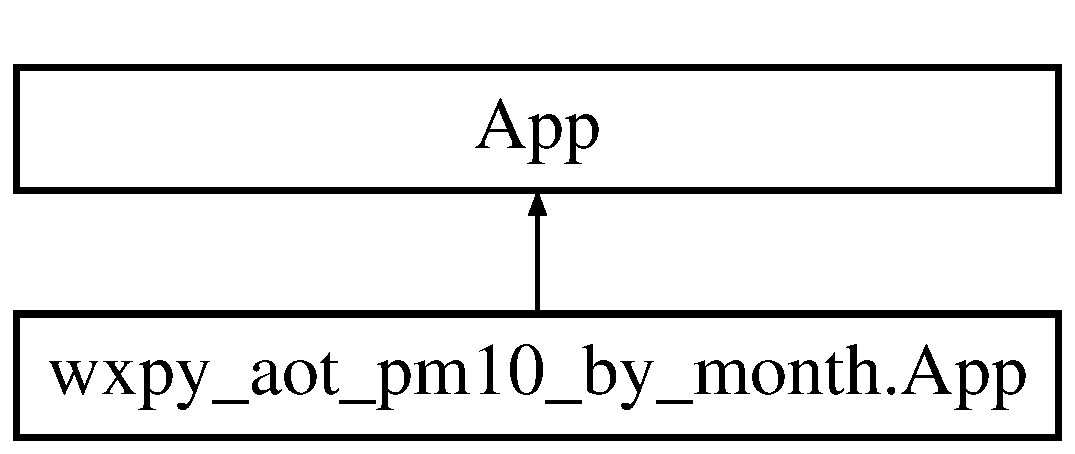
\includegraphics[height=2.000000cm]{classwxpy__aot__pm10__by__month_1_1_app}
\end{center}
\end{figure}
\subsection*{Fonctions membres publiques}
\begin{DoxyCompactItemize}
\item 
def \hyperlink{classwxpy__aot__pm10__by__month_1_1_app_a437fdfe69603140d04ddda7b3a18d731}{On\-Init}
\end{DoxyCompactItemize}


\subsection{Documentation des fonctions membres}
\hypertarget{classwxpy__aot__pm10__by__month_1_1_app_a437fdfe69603140d04ddda7b3a18d731}{\index{wxpy\-\_\-aot\-\_\-pm10\-\_\-by\-\_\-month\-::\-App@{wxpy\-\_\-aot\-\_\-pm10\-\_\-by\-\_\-month\-::\-App}!On\-Init@{On\-Init}}
\index{On\-Init@{On\-Init}!wxpy_aot_pm10_by_month::App@{wxpy\-\_\-aot\-\_\-pm10\-\_\-by\-\_\-month\-::\-App}}
\subsubsection[{On\-Init}]{\setlength{\rightskip}{0pt plus 5cm}def wxpy\-\_\-aot\-\_\-pm10\-\_\-by\-\_\-month.\-App.\-On\-Init (
\begin{DoxyParamCaption}
\item[{}]{self}
\end{DoxyParamCaption}
)}}\label{classwxpy__aot__pm10__by__month_1_1_app_a437fdfe69603140d04ddda7b3a18d731}


La documentation de cette classe a été générée à partir du fichier suivant \-:\begin{DoxyCompactItemize}
\item 
\hyperlink{wxpy__aot__pm10__by__month_8py}{wxpy\-\_\-aot\-\_\-pm10\-\_\-by\-\_\-month.\-py}\end{DoxyCompactItemize}

\hypertarget{classwxpy__aot__pm10__by__years_1_1_app}{\section{Référence de la classe wxpy\-\_\-aot\-\_\-pm10\-\_\-by\-\_\-years.\-App}
\label{classwxpy__aot__pm10__by__years_1_1_app}\index{wxpy\-\_\-aot\-\_\-pm10\-\_\-by\-\_\-years.\-App@{wxpy\-\_\-aot\-\_\-pm10\-\_\-by\-\_\-years.\-App}}
}
Graphe d'héritage de wxpy\-\_\-aot\-\_\-pm10\-\_\-by\-\_\-years.\-App\-:\begin{figure}[H]
\begin{center}
\leavevmode
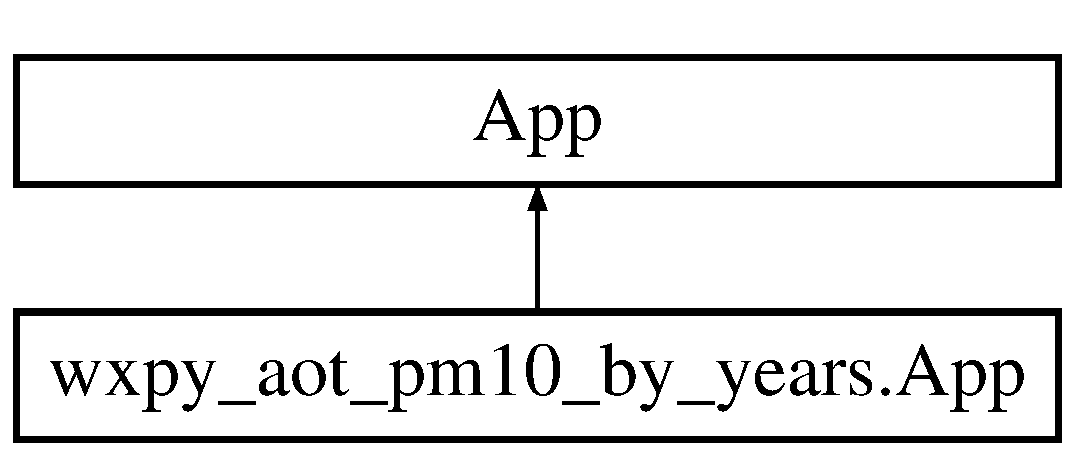
\includegraphics[height=2.000000cm]{classwxpy__aot__pm10__by__years_1_1_app}
\end{center}
\end{figure}
\subsection*{Fonctions membres publiques}
\begin{DoxyCompactItemize}
\item 
def \hyperlink{classwxpy__aot__pm10__by__years_1_1_app_ae17bc17f9f58f8e8bda96c06f0d44334}{On\-Init}
\end{DoxyCompactItemize}


\subsection{Documentation des fonctions membres}
\hypertarget{classwxpy__aot__pm10__by__years_1_1_app_ae17bc17f9f58f8e8bda96c06f0d44334}{\index{wxpy\-\_\-aot\-\_\-pm10\-\_\-by\-\_\-years\-::\-App@{wxpy\-\_\-aot\-\_\-pm10\-\_\-by\-\_\-years\-::\-App}!On\-Init@{On\-Init}}
\index{On\-Init@{On\-Init}!wxpy_aot_pm10_by_years::App@{wxpy\-\_\-aot\-\_\-pm10\-\_\-by\-\_\-years\-::\-App}}
\subsubsection[{On\-Init}]{\setlength{\rightskip}{0pt plus 5cm}def wxpy\-\_\-aot\-\_\-pm10\-\_\-by\-\_\-years.\-App.\-On\-Init (
\begin{DoxyParamCaption}
\item[{}]{self}
\end{DoxyParamCaption}
)}}\label{classwxpy__aot__pm10__by__years_1_1_app_ae17bc17f9f58f8e8bda96c06f0d44334}


La documentation de cette classe a été générée à partir du fichier suivant \-:\begin{DoxyCompactItemize}
\item 
\hyperlink{wxpy__aot__pm10__by__years_8py}{wxpy\-\_\-aot\-\_\-pm10\-\_\-by\-\_\-years.\-py}\end{DoxyCompactItemize}

\hypertarget{classwxpy__aot__pm10__by__year__sep__x__2009__v2_1_1_app}{\section{Référence de la classe wxpy\-\_\-aot\-\_\-pm10\-\_\-by\-\_\-year\-\_\-sep\-\_\-x\-\_\-2009\-\_\-v2.\-App}
\label{classwxpy__aot__pm10__by__year__sep__x__2009__v2_1_1_app}\index{wxpy\-\_\-aot\-\_\-pm10\-\_\-by\-\_\-year\-\_\-sep\-\_\-x\-\_\-2009\-\_\-v2.\-App@{wxpy\-\_\-aot\-\_\-pm10\-\_\-by\-\_\-year\-\_\-sep\-\_\-x\-\_\-2009\-\_\-v2.\-App}}
}
Graphe d'héritage de wxpy\-\_\-aot\-\_\-pm10\-\_\-by\-\_\-year\-\_\-sep\-\_\-x\-\_\-2009\-\_\-v2.\-App\-:\begin{figure}[H]
\begin{center}
\leavevmode
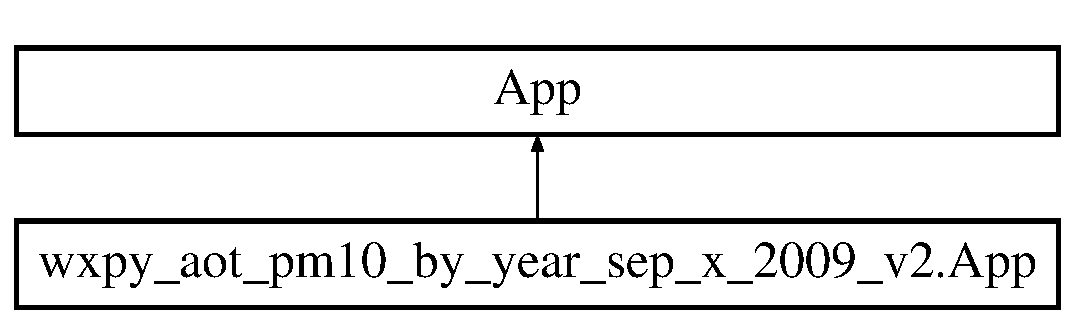
\includegraphics[height=2.000000cm]{classwxpy__aot__pm10__by__year__sep__x__2009__v2_1_1_app}
\end{center}
\end{figure}
\subsection*{Fonctions membres publiques}
\begin{DoxyCompactItemize}
\item 
def \hyperlink{classwxpy__aot__pm10__by__year__sep__x__2009__v2_1_1_app_a723681405ef3699aba954cc88469f9ad}{On\-Init}
\end{DoxyCompactItemize}


\subsection{Documentation des fonctions membres}
\hypertarget{classwxpy__aot__pm10__by__year__sep__x__2009__v2_1_1_app_a723681405ef3699aba954cc88469f9ad}{\index{wxpy\-\_\-aot\-\_\-pm10\-\_\-by\-\_\-year\-\_\-sep\-\_\-x\-\_\-2009\-\_\-v2\-::\-App@{wxpy\-\_\-aot\-\_\-pm10\-\_\-by\-\_\-year\-\_\-sep\-\_\-x\-\_\-2009\-\_\-v2\-::\-App}!On\-Init@{On\-Init}}
\index{On\-Init@{On\-Init}!wxpy_aot_pm10_by_year_sep_x_2009_v2::App@{wxpy\-\_\-aot\-\_\-pm10\-\_\-by\-\_\-year\-\_\-sep\-\_\-x\-\_\-2009\-\_\-v2\-::\-App}}
\subsubsection[{On\-Init}]{\setlength{\rightskip}{0pt plus 5cm}def wxpy\-\_\-aot\-\_\-pm10\-\_\-by\-\_\-year\-\_\-sep\-\_\-x\-\_\-2009\-\_\-v2.\-App.\-On\-Init (
\begin{DoxyParamCaption}
\item[{}]{self}
\end{DoxyParamCaption}
)}}\label{classwxpy__aot__pm10__by__year__sep__x__2009__v2_1_1_app_a723681405ef3699aba954cc88469f9ad}


La documentation de cette classe a été générée à partir du fichier suivant \-:\begin{DoxyCompactItemize}
\item 
\hyperlink{wxpy__aot__pm10__by__year__sep__x__2009__v2_8py}{wxpy\-\_\-aot\-\_\-pm10\-\_\-by\-\_\-year\-\_\-sep\-\_\-x\-\_\-2009\-\_\-v2.\-py}\end{DoxyCompactItemize}

\hypertarget{classwxpy__aot__pm10__by__years_1_1_canvas_frame}{\section{Référence de la classe wxpy\-\_\-aot\-\_\-pm10\-\_\-by\-\_\-years.\-Canvas\-Frame}
\label{classwxpy__aot__pm10__by__years_1_1_canvas_frame}\index{wxpy\-\_\-aot\-\_\-pm10\-\_\-by\-\_\-years.\-Canvas\-Frame@{wxpy\-\_\-aot\-\_\-pm10\-\_\-by\-\_\-years.\-Canvas\-Frame}}
}
Graphe d'héritage de wxpy\-\_\-aot\-\_\-pm10\-\_\-by\-\_\-years.\-Canvas\-Frame\-:\begin{figure}[H]
\begin{center}
\leavevmode
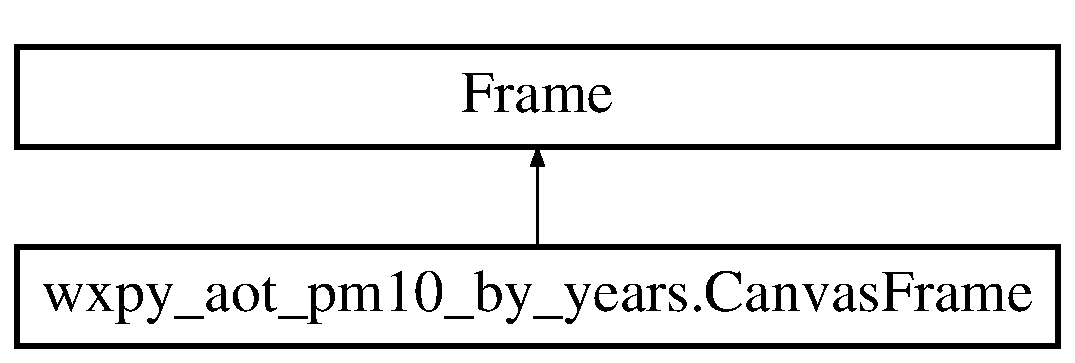
\includegraphics[height=2.000000cm]{classwxpy__aot__pm10__by__years_1_1_canvas_frame}
\end{center}
\end{figure}
\subsection*{Fonctions membres publiques}
\begin{DoxyCompactItemize}
\item 
def \hyperlink{classwxpy__aot__pm10__by__years_1_1_canvas_frame_a4fadc42c5393da9736616bf289bba7ba}{\-\_\-\-\_\-init\-\_\-\-\_\-}
\item 
def \hyperlink{classwxpy__aot__pm10__by__years_1_1_canvas_frame_a7fb754f6cd5f7f2378b47c9e8ee94182}{Init\-Config}
\item 
def \hyperlink{classwxpy__aot__pm10__by__years_1_1_canvas_frame_a447c04b919876bf2bdb1e5d36757b574}{unique}
\item 
def \hyperlink{classwxpy__aot__pm10__by__years_1_1_canvas_frame_a6818fd4490498c9bd4864011ee1f74b8}{Prep\-Data}
\item 
def \hyperlink{classwxpy__aot__pm10__by__years_1_1_canvas_frame_a0dce44581c1fe2189deb16131c96bc92}{On\-Clicked}
\item 
def \hyperlink{classwxpy__aot__pm10__by__years_1_1_canvas_frame_ab08785b0b9a6e5746f66b176a04e37f3}{On\-Paint}
\item 
def \hyperlink{classwxpy__aot__pm10__by__years_1_1_canvas_frame_af26d9c13d57da71653971111777493be}{On\-Shell}
\item 
def \hyperlink{classwxpy__aot__pm10__by__years_1_1_canvas_frame_a208b24536707d450ed18dad6d0aefa09}{On\-Filling}
\item 
def \hyperlink{classwxpy__aot__pm10__by__years_1_1_canvas_frame_ace0afe2826dd3d115d3b7801d8b760f6}{On\-Exit}
\item 
def \hyperlink{classwxpy__aot__pm10__by__years_1_1_canvas_frame_a0672189a685aa7d5cf7b639deda6b072}{On\-Options}
\end{DoxyCompactItemize}
\subsection*{Attributs publics}
\begin{DoxyCompactItemize}
\item 
\hyperlink{classwxpy__aot__pm10__by__years_1_1_canvas_frame_a32074c912b904491fbcdd429bd3637f9}{figure}
\item 
\hyperlink{classwxpy__aot__pm10__by__years_1_1_canvas_frame_ad8c14ace813e031fb6fbaa1e92830f5f}{initdir}
\item 
\hyperlink{classwxpy__aot__pm10__by__years_1_1_canvas_frame_a7ed3a9acc45420fcdc01decddd24d818}{canvas}
\item 
\hyperlink{classwxpy__aot__pm10__by__years_1_1_canvas_frame_a4cd3730e0e6b668107b910e98fa045ee}{sizer}
\item 
\hyperlink{classwxpy__aot__pm10__by__years_1_1_canvas_frame_a89adfebea2e1a6f6cb558a92578b78c9}{b\-Change\-Config}
\item 
\hyperlink{classwxpy__aot__pm10__by__years_1_1_canvas_frame_a63ff15b073da1b6264169eb4d569d77e}{toolbar}
\item 
\hyperlink{classwxpy__aot__pm10__by__years_1_1_canvas_frame_a60b48a121123885e55fa2398bcb26bff}{Config}
\end{DoxyCompactItemize}


\subsection{Description détaillée}
\begin{DoxyVerb}Classe CanvasFrame \end{DoxyVerb}
 

\subsection{Documentation des constructeurs et destructeur}
\hypertarget{classwxpy__aot__pm10__by__years_1_1_canvas_frame_a4fadc42c5393da9736616bf289bba7ba}{\index{wxpy\-\_\-aot\-\_\-pm10\-\_\-by\-\_\-years\-::\-Canvas\-Frame@{wxpy\-\_\-aot\-\_\-pm10\-\_\-by\-\_\-years\-::\-Canvas\-Frame}!\-\_\-\-\_\-init\-\_\-\-\_\-@{\-\_\-\-\_\-init\-\_\-\-\_\-}}
\index{\-\_\-\-\_\-init\-\_\-\-\_\-@{\-\_\-\-\_\-init\-\_\-\-\_\-}!wxpy_aot_pm10_by_years::CanvasFrame@{wxpy\-\_\-aot\-\_\-pm10\-\_\-by\-\_\-years\-::\-Canvas\-Frame}}
\subsubsection[{\-\_\-\-\_\-init\-\_\-\-\_\-}]{\setlength{\rightskip}{0pt plus 5cm}def wxpy\-\_\-aot\-\_\-pm10\-\_\-by\-\_\-years.\-Canvas\-Frame.\-\_\-\-\_\-init\-\_\-\-\_\- (
\begin{DoxyParamCaption}
\item[{}]{self}
\end{DoxyParamCaption}
)}}\label{classwxpy__aot__pm10__by__years_1_1_canvas_frame_a4fadc42c5393da9736616bf289bba7ba}


\subsection{Documentation des fonctions membres}
\hypertarget{classwxpy__aot__pm10__by__years_1_1_canvas_frame_a7fb754f6cd5f7f2378b47c9e8ee94182}{\index{wxpy\-\_\-aot\-\_\-pm10\-\_\-by\-\_\-years\-::\-Canvas\-Frame@{wxpy\-\_\-aot\-\_\-pm10\-\_\-by\-\_\-years\-::\-Canvas\-Frame}!Init\-Config@{Init\-Config}}
\index{Init\-Config@{Init\-Config}!wxpy_aot_pm10_by_years::CanvasFrame@{wxpy\-\_\-aot\-\_\-pm10\-\_\-by\-\_\-years\-::\-Canvas\-Frame}}
\subsubsection[{Init\-Config}]{\setlength{\rightskip}{0pt plus 5cm}def wxpy\-\_\-aot\-\_\-pm10\-\_\-by\-\_\-years.\-Canvas\-Frame.\-Init\-Config (
\begin{DoxyParamCaption}
\item[{}]{self}
\end{DoxyParamCaption}
)}}\label{classwxpy__aot__pm10__by__years_1_1_canvas_frame_a7fb754f6cd5f7f2378b47c9e8ee94182}
\hypertarget{classwxpy__aot__pm10__by__years_1_1_canvas_frame_a0dce44581c1fe2189deb16131c96bc92}{\index{wxpy\-\_\-aot\-\_\-pm10\-\_\-by\-\_\-years\-::\-Canvas\-Frame@{wxpy\-\_\-aot\-\_\-pm10\-\_\-by\-\_\-years\-::\-Canvas\-Frame}!On\-Clicked@{On\-Clicked}}
\index{On\-Clicked@{On\-Clicked}!wxpy_aot_pm10_by_years::CanvasFrame@{wxpy\-\_\-aot\-\_\-pm10\-\_\-by\-\_\-years\-::\-Canvas\-Frame}}
\subsubsection[{On\-Clicked}]{\setlength{\rightskip}{0pt plus 5cm}def wxpy\-\_\-aot\-\_\-pm10\-\_\-by\-\_\-years.\-Canvas\-Frame.\-On\-Clicked (
\begin{DoxyParamCaption}
\item[{}]{self, }
\item[{}]{event}
\end{DoxyParamCaption}
)}}\label{classwxpy__aot__pm10__by__years_1_1_canvas_frame_a0dce44581c1fe2189deb16131c96bc92}
\hypertarget{classwxpy__aot__pm10__by__years_1_1_canvas_frame_ace0afe2826dd3d115d3b7801d8b760f6}{\index{wxpy\-\_\-aot\-\_\-pm10\-\_\-by\-\_\-years\-::\-Canvas\-Frame@{wxpy\-\_\-aot\-\_\-pm10\-\_\-by\-\_\-years\-::\-Canvas\-Frame}!On\-Exit@{On\-Exit}}
\index{On\-Exit@{On\-Exit}!wxpy_aot_pm10_by_years::CanvasFrame@{wxpy\-\_\-aot\-\_\-pm10\-\_\-by\-\_\-years\-::\-Canvas\-Frame}}
\subsubsection[{On\-Exit}]{\setlength{\rightskip}{0pt plus 5cm}def wxpy\-\_\-aot\-\_\-pm10\-\_\-by\-\_\-years.\-Canvas\-Frame.\-On\-Exit (
\begin{DoxyParamCaption}
\item[{}]{self, }
\item[{}]{event}
\end{DoxyParamCaption}
)}}\label{classwxpy__aot__pm10__by__years_1_1_canvas_frame_ace0afe2826dd3d115d3b7801d8b760f6}
\hypertarget{classwxpy__aot__pm10__by__years_1_1_canvas_frame_a208b24536707d450ed18dad6d0aefa09}{\index{wxpy\-\_\-aot\-\_\-pm10\-\_\-by\-\_\-years\-::\-Canvas\-Frame@{wxpy\-\_\-aot\-\_\-pm10\-\_\-by\-\_\-years\-::\-Canvas\-Frame}!On\-Filling@{On\-Filling}}
\index{On\-Filling@{On\-Filling}!wxpy_aot_pm10_by_years::CanvasFrame@{wxpy\-\_\-aot\-\_\-pm10\-\_\-by\-\_\-years\-::\-Canvas\-Frame}}
\subsubsection[{On\-Filling}]{\setlength{\rightskip}{0pt plus 5cm}def wxpy\-\_\-aot\-\_\-pm10\-\_\-by\-\_\-years.\-Canvas\-Frame.\-On\-Filling (
\begin{DoxyParamCaption}
\item[{}]{self, }
\item[{}]{event}
\end{DoxyParamCaption}
)}}\label{classwxpy__aot__pm10__by__years_1_1_canvas_frame_a208b24536707d450ed18dad6d0aefa09}
\begin{DoxyVerb}Browser pycrust \end{DoxyVerb}
 \hypertarget{classwxpy__aot__pm10__by__years_1_1_canvas_frame_a0672189a685aa7d5cf7b639deda6b072}{\index{wxpy\-\_\-aot\-\_\-pm10\-\_\-by\-\_\-years\-::\-Canvas\-Frame@{wxpy\-\_\-aot\-\_\-pm10\-\_\-by\-\_\-years\-::\-Canvas\-Frame}!On\-Options@{On\-Options}}
\index{On\-Options@{On\-Options}!wxpy_aot_pm10_by_years::CanvasFrame@{wxpy\-\_\-aot\-\_\-pm10\-\_\-by\-\_\-years\-::\-Canvas\-Frame}}
\subsubsection[{On\-Options}]{\setlength{\rightskip}{0pt plus 5cm}def wxpy\-\_\-aot\-\_\-pm10\-\_\-by\-\_\-years.\-Canvas\-Frame.\-On\-Options (
\begin{DoxyParamCaption}
\item[{}]{self, }
\item[{}]{event}
\end{DoxyParamCaption}
)}}\label{classwxpy__aot__pm10__by__years_1_1_canvas_frame_a0672189a685aa7d5cf7b639deda6b072}
\begin{DoxyVerb}Parameters Dialog Handler \end{DoxyVerb}
 \hypertarget{classwxpy__aot__pm10__by__years_1_1_canvas_frame_ab08785b0b9a6e5746f66b176a04e37f3}{\index{wxpy\-\_\-aot\-\_\-pm10\-\_\-by\-\_\-years\-::\-Canvas\-Frame@{wxpy\-\_\-aot\-\_\-pm10\-\_\-by\-\_\-years\-::\-Canvas\-Frame}!On\-Paint@{On\-Paint}}
\index{On\-Paint@{On\-Paint}!wxpy_aot_pm10_by_years::CanvasFrame@{wxpy\-\_\-aot\-\_\-pm10\-\_\-by\-\_\-years\-::\-Canvas\-Frame}}
\subsubsection[{On\-Paint}]{\setlength{\rightskip}{0pt plus 5cm}def wxpy\-\_\-aot\-\_\-pm10\-\_\-by\-\_\-years.\-Canvas\-Frame.\-On\-Paint (
\begin{DoxyParamCaption}
\item[{}]{self, }
\item[{}]{event}
\end{DoxyParamCaption}
)}}\label{classwxpy__aot__pm10__by__years_1_1_canvas_frame_ab08785b0b9a6e5746f66b176a04e37f3}
\hypertarget{classwxpy__aot__pm10__by__years_1_1_canvas_frame_af26d9c13d57da71653971111777493be}{\index{wxpy\-\_\-aot\-\_\-pm10\-\_\-by\-\_\-years\-::\-Canvas\-Frame@{wxpy\-\_\-aot\-\_\-pm10\-\_\-by\-\_\-years\-::\-Canvas\-Frame}!On\-Shell@{On\-Shell}}
\index{On\-Shell@{On\-Shell}!wxpy_aot_pm10_by_years::CanvasFrame@{wxpy\-\_\-aot\-\_\-pm10\-\_\-by\-\_\-years\-::\-Canvas\-Frame}}
\subsubsection[{On\-Shell}]{\setlength{\rightskip}{0pt plus 5cm}def wxpy\-\_\-aot\-\_\-pm10\-\_\-by\-\_\-years.\-Canvas\-Frame.\-On\-Shell (
\begin{DoxyParamCaption}
\item[{}]{self, }
\item[{}]{event}
\end{DoxyParamCaption}
)}}\label{classwxpy__aot__pm10__by__years_1_1_canvas_frame_af26d9c13d57da71653971111777493be}
\begin{DoxyVerb}Shell pycrust \end{DoxyVerb}
 \hypertarget{classwxpy__aot__pm10__by__years_1_1_canvas_frame_a6818fd4490498c9bd4864011ee1f74b8}{\index{wxpy\-\_\-aot\-\_\-pm10\-\_\-by\-\_\-years\-::\-Canvas\-Frame@{wxpy\-\_\-aot\-\_\-pm10\-\_\-by\-\_\-years\-::\-Canvas\-Frame}!Prep\-Data@{Prep\-Data}}
\index{Prep\-Data@{Prep\-Data}!wxpy_aot_pm10_by_years::CanvasFrame@{wxpy\-\_\-aot\-\_\-pm10\-\_\-by\-\_\-years\-::\-Canvas\-Frame}}
\subsubsection[{Prep\-Data}]{\setlength{\rightskip}{0pt plus 5cm}def wxpy\-\_\-aot\-\_\-pm10\-\_\-by\-\_\-years.\-Canvas\-Frame.\-Prep\-Data (
\begin{DoxyParamCaption}
\item[{}]{self}
\end{DoxyParamCaption}
)}}\label{classwxpy__aot__pm10__by__years_1_1_canvas_frame_a6818fd4490498c9bd4864011ee1f74b8}
\begin{DoxyVerb}Prepare data before plotting \end{DoxyVerb}
 \hypertarget{classwxpy__aot__pm10__by__years_1_1_canvas_frame_a447c04b919876bf2bdb1e5d36757b574}{\index{wxpy\-\_\-aot\-\_\-pm10\-\_\-by\-\_\-years\-::\-Canvas\-Frame@{wxpy\-\_\-aot\-\_\-pm10\-\_\-by\-\_\-years\-::\-Canvas\-Frame}!unique@{unique}}
\index{unique@{unique}!wxpy_aot_pm10_by_years::CanvasFrame@{wxpy\-\_\-aot\-\_\-pm10\-\_\-by\-\_\-years\-::\-Canvas\-Frame}}
\subsubsection[{unique}]{\setlength{\rightskip}{0pt plus 5cm}def wxpy\-\_\-aot\-\_\-pm10\-\_\-by\-\_\-years.\-Canvas\-Frame.\-unique (
\begin{DoxyParamCaption}
\item[{}]{self, }
\item[{}]{a}
\end{DoxyParamCaption}
)}}\label{classwxpy__aot__pm10__by__years_1_1_canvas_frame_a447c04b919876bf2bdb1e5d36757b574}
\begin{DoxyVerb}Renvoie un vecteur contenant les valeurs uniques d'un vecteur  \end{DoxyVerb}
 

\subsection{Documentation des données membres}
\hypertarget{classwxpy__aot__pm10__by__years_1_1_canvas_frame_a89adfebea2e1a6f6cb558a92578b78c9}{\index{wxpy\-\_\-aot\-\_\-pm10\-\_\-by\-\_\-years\-::\-Canvas\-Frame@{wxpy\-\_\-aot\-\_\-pm10\-\_\-by\-\_\-years\-::\-Canvas\-Frame}!b\-Change\-Config@{b\-Change\-Config}}
\index{b\-Change\-Config@{b\-Change\-Config}!wxpy_aot_pm10_by_years::CanvasFrame@{wxpy\-\_\-aot\-\_\-pm10\-\_\-by\-\_\-years\-::\-Canvas\-Frame}}
\subsubsection[{b\-Change\-Config}]{\setlength{\rightskip}{0pt plus 5cm}wxpy\-\_\-aot\-\_\-pm10\-\_\-by\-\_\-years.\-Canvas\-Frame.\-b\-Change\-Config}}\label{classwxpy__aot__pm10__by__years_1_1_canvas_frame_a89adfebea2e1a6f6cb558a92578b78c9}
\hypertarget{classwxpy__aot__pm10__by__years_1_1_canvas_frame_a7ed3a9acc45420fcdc01decddd24d818}{\index{wxpy\-\_\-aot\-\_\-pm10\-\_\-by\-\_\-years\-::\-Canvas\-Frame@{wxpy\-\_\-aot\-\_\-pm10\-\_\-by\-\_\-years\-::\-Canvas\-Frame}!canvas@{canvas}}
\index{canvas@{canvas}!wxpy_aot_pm10_by_years::CanvasFrame@{wxpy\-\_\-aot\-\_\-pm10\-\_\-by\-\_\-years\-::\-Canvas\-Frame}}
\subsubsection[{canvas}]{\setlength{\rightskip}{0pt plus 5cm}wxpy\-\_\-aot\-\_\-pm10\-\_\-by\-\_\-years.\-Canvas\-Frame.\-canvas}}\label{classwxpy__aot__pm10__by__years_1_1_canvas_frame_a7ed3a9acc45420fcdc01decddd24d818}
\hypertarget{classwxpy__aot__pm10__by__years_1_1_canvas_frame_a60b48a121123885e55fa2398bcb26bff}{\index{wxpy\-\_\-aot\-\_\-pm10\-\_\-by\-\_\-years\-::\-Canvas\-Frame@{wxpy\-\_\-aot\-\_\-pm10\-\_\-by\-\_\-years\-::\-Canvas\-Frame}!Config@{Config}}
\index{Config@{Config}!wxpy_aot_pm10_by_years::CanvasFrame@{wxpy\-\_\-aot\-\_\-pm10\-\_\-by\-\_\-years\-::\-Canvas\-Frame}}
\subsubsection[{Config}]{\setlength{\rightskip}{0pt plus 5cm}wxpy\-\_\-aot\-\_\-pm10\-\_\-by\-\_\-years.\-Canvas\-Frame.\-Config}}\label{classwxpy__aot__pm10__by__years_1_1_canvas_frame_a60b48a121123885e55fa2398bcb26bff}
\hypertarget{classwxpy__aot__pm10__by__years_1_1_canvas_frame_a32074c912b904491fbcdd429bd3637f9}{\index{wxpy\-\_\-aot\-\_\-pm10\-\_\-by\-\_\-years\-::\-Canvas\-Frame@{wxpy\-\_\-aot\-\_\-pm10\-\_\-by\-\_\-years\-::\-Canvas\-Frame}!figure@{figure}}
\index{figure@{figure}!wxpy_aot_pm10_by_years::CanvasFrame@{wxpy\-\_\-aot\-\_\-pm10\-\_\-by\-\_\-years\-::\-Canvas\-Frame}}
\subsubsection[{figure}]{\setlength{\rightskip}{0pt plus 5cm}wxpy\-\_\-aot\-\_\-pm10\-\_\-by\-\_\-years.\-Canvas\-Frame.\-figure}}\label{classwxpy__aot__pm10__by__years_1_1_canvas_frame_a32074c912b904491fbcdd429bd3637f9}
\hypertarget{classwxpy__aot__pm10__by__years_1_1_canvas_frame_ad8c14ace813e031fb6fbaa1e92830f5f}{\index{wxpy\-\_\-aot\-\_\-pm10\-\_\-by\-\_\-years\-::\-Canvas\-Frame@{wxpy\-\_\-aot\-\_\-pm10\-\_\-by\-\_\-years\-::\-Canvas\-Frame}!initdir@{initdir}}
\index{initdir@{initdir}!wxpy_aot_pm10_by_years::CanvasFrame@{wxpy\-\_\-aot\-\_\-pm10\-\_\-by\-\_\-years\-::\-Canvas\-Frame}}
\subsubsection[{initdir}]{\setlength{\rightskip}{0pt plus 5cm}wxpy\-\_\-aot\-\_\-pm10\-\_\-by\-\_\-years.\-Canvas\-Frame.\-initdir}}\label{classwxpy__aot__pm10__by__years_1_1_canvas_frame_ad8c14ace813e031fb6fbaa1e92830f5f}
\hypertarget{classwxpy__aot__pm10__by__years_1_1_canvas_frame_a4cd3730e0e6b668107b910e98fa045ee}{\index{wxpy\-\_\-aot\-\_\-pm10\-\_\-by\-\_\-years\-::\-Canvas\-Frame@{wxpy\-\_\-aot\-\_\-pm10\-\_\-by\-\_\-years\-::\-Canvas\-Frame}!sizer@{sizer}}
\index{sizer@{sizer}!wxpy_aot_pm10_by_years::CanvasFrame@{wxpy\-\_\-aot\-\_\-pm10\-\_\-by\-\_\-years\-::\-Canvas\-Frame}}
\subsubsection[{sizer}]{\setlength{\rightskip}{0pt plus 5cm}wxpy\-\_\-aot\-\_\-pm10\-\_\-by\-\_\-years.\-Canvas\-Frame.\-sizer}}\label{classwxpy__aot__pm10__by__years_1_1_canvas_frame_a4cd3730e0e6b668107b910e98fa045ee}
\hypertarget{classwxpy__aot__pm10__by__years_1_1_canvas_frame_a63ff15b073da1b6264169eb4d569d77e}{\index{wxpy\-\_\-aot\-\_\-pm10\-\_\-by\-\_\-years\-::\-Canvas\-Frame@{wxpy\-\_\-aot\-\_\-pm10\-\_\-by\-\_\-years\-::\-Canvas\-Frame}!toolbar@{toolbar}}
\index{toolbar@{toolbar}!wxpy_aot_pm10_by_years::CanvasFrame@{wxpy\-\_\-aot\-\_\-pm10\-\_\-by\-\_\-years\-::\-Canvas\-Frame}}
\subsubsection[{toolbar}]{\setlength{\rightskip}{0pt plus 5cm}wxpy\-\_\-aot\-\_\-pm10\-\_\-by\-\_\-years.\-Canvas\-Frame.\-toolbar}}\label{classwxpy__aot__pm10__by__years_1_1_canvas_frame_a63ff15b073da1b6264169eb4d569d77e}


La documentation de cette classe a été générée à partir du fichier suivant \-:\begin{DoxyCompactItemize}
\item 
\hyperlink{wxpy__aot__pm10__by__years_8py}{wxpy\-\_\-aot\-\_\-pm10\-\_\-by\-\_\-years.\-py}\end{DoxyCompactItemize}

\hypertarget{classwxpy__aot__pm10__by__year__sep__x__2009__v2_1_1_canvas_frame}{\section{Référence de la classe wxpy\-\_\-aot\-\_\-pm10\-\_\-by\-\_\-year\-\_\-sep\-\_\-x\-\_\-2009\-\_\-v2.\-Canvas\-Frame}
\label{classwxpy__aot__pm10__by__year__sep__x__2009__v2_1_1_canvas_frame}\index{wxpy\-\_\-aot\-\_\-pm10\-\_\-by\-\_\-year\-\_\-sep\-\_\-x\-\_\-2009\-\_\-v2.\-Canvas\-Frame@{wxpy\-\_\-aot\-\_\-pm10\-\_\-by\-\_\-year\-\_\-sep\-\_\-x\-\_\-2009\-\_\-v2.\-Canvas\-Frame}}
}
Graphe d'héritage de wxpy\-\_\-aot\-\_\-pm10\-\_\-by\-\_\-year\-\_\-sep\-\_\-x\-\_\-2009\-\_\-v2.\-Canvas\-Frame\-:\begin{figure}[H]
\begin{center}
\leavevmode
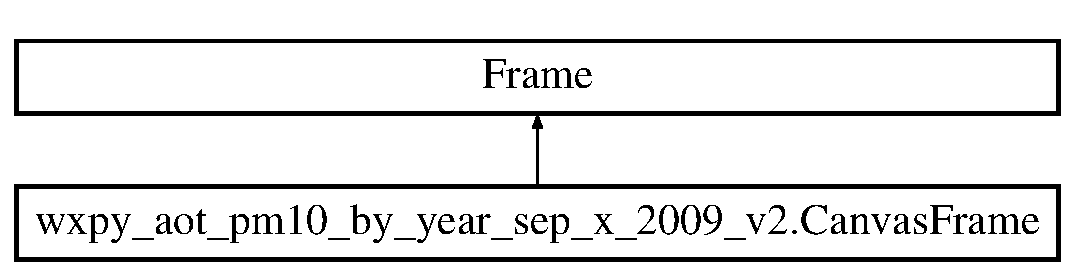
\includegraphics[height=2.000000cm]{classwxpy__aot__pm10__by__year__sep__x__2009__v2_1_1_canvas_frame}
\end{center}
\end{figure}
\subsection*{Fonctions membres publiques}
\begin{DoxyCompactItemize}
\item 
def \hyperlink{classwxpy__aot__pm10__by__year__sep__x__2009__v2_1_1_canvas_frame_a2f3402930df5b23c70a05bb2b02fecbb}{\-\_\-\-\_\-init\-\_\-\-\_\-}
\item 
def \hyperlink{classwxpy__aot__pm10__by__year__sep__x__2009__v2_1_1_canvas_frame_a4921677b5c61ea75dcf891e3aa3d2922}{Init\-Config}
\item 
def \hyperlink{classwxpy__aot__pm10__by__year__sep__x__2009__v2_1_1_canvas_frame_a58c0b0c678af77c0bb9532695088ce87}{unique}
\item 
def \hyperlink{classwxpy__aot__pm10__by__year__sep__x__2009__v2_1_1_canvas_frame_abed7d4c6d1c6bb71a74f05ca5b4efd70}{Prep\-Data}
\item 
def \hyperlink{classwxpy__aot__pm10__by__year__sep__x__2009__v2_1_1_canvas_frame_a3c6d3e08e4096e060f76cc27d1593225}{On\-Clicked}
\item 
def \hyperlink{classwxpy__aot__pm10__by__year__sep__x__2009__v2_1_1_canvas_frame_aebe11aecfef9635030426edeb0121e74}{On\-Paint}
\item 
def \hyperlink{classwxpy__aot__pm10__by__year__sep__x__2009__v2_1_1_canvas_frame_a62c6659283638fe5e86058df99ecd02a}{On\-Shell}
\item 
def \hyperlink{classwxpy__aot__pm10__by__year__sep__x__2009__v2_1_1_canvas_frame_a57994e58517d8339b7ef7f51b6631554}{On\-Filling}
\item 
def \hyperlink{classwxpy__aot__pm10__by__year__sep__x__2009__v2_1_1_canvas_frame_abb0238138da028f98cb1df5dde47c2a4}{On\-Exit}
\item 
def \hyperlink{classwxpy__aot__pm10__by__year__sep__x__2009__v2_1_1_canvas_frame_a179878bf0c7ba265837f2786fb4bfeab}{On\-Options}
\end{DoxyCompactItemize}
\subsection*{Attributs publics}
\begin{DoxyCompactItemize}
\item 
\hyperlink{classwxpy__aot__pm10__by__year__sep__x__2009__v2_1_1_canvas_frame_a8e8b2e1dea08dccf777a56d75712ffc1}{figure}
\item 
\hyperlink{classwxpy__aot__pm10__by__year__sep__x__2009__v2_1_1_canvas_frame_a1890d92f42522e9ef11e8dbed8036015}{initdir}
\item 
\hyperlink{classwxpy__aot__pm10__by__year__sep__x__2009__v2_1_1_canvas_frame_a5dd5e8441fb7d4bfdfdfdad6c0fc7c04}{canvas}
\item 
\hyperlink{classwxpy__aot__pm10__by__year__sep__x__2009__v2_1_1_canvas_frame_a2316e595af6677c1eda90fe42fc719ab}{sizer}
\item 
\hyperlink{classwxpy__aot__pm10__by__year__sep__x__2009__v2_1_1_canvas_frame_aafaee18828675aed1d9ce40917c2c1ab}{b\-Change\-Config}
\item 
\hyperlink{classwxpy__aot__pm10__by__year__sep__x__2009__v2_1_1_canvas_frame_add8b71a2663ce00a7e77b490bbed6a61}{toolbar}
\item 
\hyperlink{classwxpy__aot__pm10__by__year__sep__x__2009__v2_1_1_canvas_frame_a65c22169047e5d96f1b4a603b6e48efb}{Config}
\end{DoxyCompactItemize}


\subsection{Description détaillée}
\begin{DoxyVerb}Classe CanvasFrame \end{DoxyVerb}
 

\subsection{Documentation des constructeurs et destructeur}
\hypertarget{classwxpy__aot__pm10__by__year__sep__x__2009__v2_1_1_canvas_frame_a2f3402930df5b23c70a05bb2b02fecbb}{\index{wxpy\-\_\-aot\-\_\-pm10\-\_\-by\-\_\-year\-\_\-sep\-\_\-x\-\_\-2009\-\_\-v2\-::\-Canvas\-Frame@{wxpy\-\_\-aot\-\_\-pm10\-\_\-by\-\_\-year\-\_\-sep\-\_\-x\-\_\-2009\-\_\-v2\-::\-Canvas\-Frame}!\-\_\-\-\_\-init\-\_\-\-\_\-@{\-\_\-\-\_\-init\-\_\-\-\_\-}}
\index{\-\_\-\-\_\-init\-\_\-\-\_\-@{\-\_\-\-\_\-init\-\_\-\-\_\-}!wxpy_aot_pm10_by_year_sep_x_2009_v2::CanvasFrame@{wxpy\-\_\-aot\-\_\-pm10\-\_\-by\-\_\-year\-\_\-sep\-\_\-x\-\_\-2009\-\_\-v2\-::\-Canvas\-Frame}}
\subsubsection[{\-\_\-\-\_\-init\-\_\-\-\_\-}]{\setlength{\rightskip}{0pt plus 5cm}def wxpy\-\_\-aot\-\_\-pm10\-\_\-by\-\_\-year\-\_\-sep\-\_\-x\-\_\-2009\-\_\-v2.\-Canvas\-Frame.\-\_\-\-\_\-init\-\_\-\-\_\- (
\begin{DoxyParamCaption}
\item[{}]{self}
\end{DoxyParamCaption}
)}}\label{classwxpy__aot__pm10__by__year__sep__x__2009__v2_1_1_canvas_frame_a2f3402930df5b23c70a05bb2b02fecbb}


\subsection{Documentation des fonctions membres}
\hypertarget{classwxpy__aot__pm10__by__year__sep__x__2009__v2_1_1_canvas_frame_a4921677b5c61ea75dcf891e3aa3d2922}{\index{wxpy\-\_\-aot\-\_\-pm10\-\_\-by\-\_\-year\-\_\-sep\-\_\-x\-\_\-2009\-\_\-v2\-::\-Canvas\-Frame@{wxpy\-\_\-aot\-\_\-pm10\-\_\-by\-\_\-year\-\_\-sep\-\_\-x\-\_\-2009\-\_\-v2\-::\-Canvas\-Frame}!Init\-Config@{Init\-Config}}
\index{Init\-Config@{Init\-Config}!wxpy_aot_pm10_by_year_sep_x_2009_v2::CanvasFrame@{wxpy\-\_\-aot\-\_\-pm10\-\_\-by\-\_\-year\-\_\-sep\-\_\-x\-\_\-2009\-\_\-v2\-::\-Canvas\-Frame}}
\subsubsection[{Init\-Config}]{\setlength{\rightskip}{0pt plus 5cm}def wxpy\-\_\-aot\-\_\-pm10\-\_\-by\-\_\-year\-\_\-sep\-\_\-x\-\_\-2009\-\_\-v2.\-Canvas\-Frame.\-Init\-Config (
\begin{DoxyParamCaption}
\item[{}]{self}
\end{DoxyParamCaption}
)}}\label{classwxpy__aot__pm10__by__year__sep__x__2009__v2_1_1_canvas_frame_a4921677b5c61ea75dcf891e3aa3d2922}
\hypertarget{classwxpy__aot__pm10__by__year__sep__x__2009__v2_1_1_canvas_frame_a3c6d3e08e4096e060f76cc27d1593225}{\index{wxpy\-\_\-aot\-\_\-pm10\-\_\-by\-\_\-year\-\_\-sep\-\_\-x\-\_\-2009\-\_\-v2\-::\-Canvas\-Frame@{wxpy\-\_\-aot\-\_\-pm10\-\_\-by\-\_\-year\-\_\-sep\-\_\-x\-\_\-2009\-\_\-v2\-::\-Canvas\-Frame}!On\-Clicked@{On\-Clicked}}
\index{On\-Clicked@{On\-Clicked}!wxpy_aot_pm10_by_year_sep_x_2009_v2::CanvasFrame@{wxpy\-\_\-aot\-\_\-pm10\-\_\-by\-\_\-year\-\_\-sep\-\_\-x\-\_\-2009\-\_\-v2\-::\-Canvas\-Frame}}
\subsubsection[{On\-Clicked}]{\setlength{\rightskip}{0pt plus 5cm}def wxpy\-\_\-aot\-\_\-pm10\-\_\-by\-\_\-year\-\_\-sep\-\_\-x\-\_\-2009\-\_\-v2.\-Canvas\-Frame.\-On\-Clicked (
\begin{DoxyParamCaption}
\item[{}]{self, }
\item[{}]{event}
\end{DoxyParamCaption}
)}}\label{classwxpy__aot__pm10__by__year__sep__x__2009__v2_1_1_canvas_frame_a3c6d3e08e4096e060f76cc27d1593225}
\hypertarget{classwxpy__aot__pm10__by__year__sep__x__2009__v2_1_1_canvas_frame_abb0238138da028f98cb1df5dde47c2a4}{\index{wxpy\-\_\-aot\-\_\-pm10\-\_\-by\-\_\-year\-\_\-sep\-\_\-x\-\_\-2009\-\_\-v2\-::\-Canvas\-Frame@{wxpy\-\_\-aot\-\_\-pm10\-\_\-by\-\_\-year\-\_\-sep\-\_\-x\-\_\-2009\-\_\-v2\-::\-Canvas\-Frame}!On\-Exit@{On\-Exit}}
\index{On\-Exit@{On\-Exit}!wxpy_aot_pm10_by_year_sep_x_2009_v2::CanvasFrame@{wxpy\-\_\-aot\-\_\-pm10\-\_\-by\-\_\-year\-\_\-sep\-\_\-x\-\_\-2009\-\_\-v2\-::\-Canvas\-Frame}}
\subsubsection[{On\-Exit}]{\setlength{\rightskip}{0pt plus 5cm}def wxpy\-\_\-aot\-\_\-pm10\-\_\-by\-\_\-year\-\_\-sep\-\_\-x\-\_\-2009\-\_\-v2.\-Canvas\-Frame.\-On\-Exit (
\begin{DoxyParamCaption}
\item[{}]{self, }
\item[{}]{event}
\end{DoxyParamCaption}
)}}\label{classwxpy__aot__pm10__by__year__sep__x__2009__v2_1_1_canvas_frame_abb0238138da028f98cb1df5dde47c2a4}
\hypertarget{classwxpy__aot__pm10__by__year__sep__x__2009__v2_1_1_canvas_frame_a57994e58517d8339b7ef7f51b6631554}{\index{wxpy\-\_\-aot\-\_\-pm10\-\_\-by\-\_\-year\-\_\-sep\-\_\-x\-\_\-2009\-\_\-v2\-::\-Canvas\-Frame@{wxpy\-\_\-aot\-\_\-pm10\-\_\-by\-\_\-year\-\_\-sep\-\_\-x\-\_\-2009\-\_\-v2\-::\-Canvas\-Frame}!On\-Filling@{On\-Filling}}
\index{On\-Filling@{On\-Filling}!wxpy_aot_pm10_by_year_sep_x_2009_v2::CanvasFrame@{wxpy\-\_\-aot\-\_\-pm10\-\_\-by\-\_\-year\-\_\-sep\-\_\-x\-\_\-2009\-\_\-v2\-::\-Canvas\-Frame}}
\subsubsection[{On\-Filling}]{\setlength{\rightskip}{0pt plus 5cm}def wxpy\-\_\-aot\-\_\-pm10\-\_\-by\-\_\-year\-\_\-sep\-\_\-x\-\_\-2009\-\_\-v2.\-Canvas\-Frame.\-On\-Filling (
\begin{DoxyParamCaption}
\item[{}]{self, }
\item[{}]{event}
\end{DoxyParamCaption}
)}}\label{classwxpy__aot__pm10__by__year__sep__x__2009__v2_1_1_canvas_frame_a57994e58517d8339b7ef7f51b6631554}
\begin{DoxyVerb}Browser pycrust \end{DoxyVerb}
 \hypertarget{classwxpy__aot__pm10__by__year__sep__x__2009__v2_1_1_canvas_frame_a179878bf0c7ba265837f2786fb4bfeab}{\index{wxpy\-\_\-aot\-\_\-pm10\-\_\-by\-\_\-year\-\_\-sep\-\_\-x\-\_\-2009\-\_\-v2\-::\-Canvas\-Frame@{wxpy\-\_\-aot\-\_\-pm10\-\_\-by\-\_\-year\-\_\-sep\-\_\-x\-\_\-2009\-\_\-v2\-::\-Canvas\-Frame}!On\-Options@{On\-Options}}
\index{On\-Options@{On\-Options}!wxpy_aot_pm10_by_year_sep_x_2009_v2::CanvasFrame@{wxpy\-\_\-aot\-\_\-pm10\-\_\-by\-\_\-year\-\_\-sep\-\_\-x\-\_\-2009\-\_\-v2\-::\-Canvas\-Frame}}
\subsubsection[{On\-Options}]{\setlength{\rightskip}{0pt plus 5cm}def wxpy\-\_\-aot\-\_\-pm10\-\_\-by\-\_\-year\-\_\-sep\-\_\-x\-\_\-2009\-\_\-v2.\-Canvas\-Frame.\-On\-Options (
\begin{DoxyParamCaption}
\item[{}]{self, }
\item[{}]{event}
\end{DoxyParamCaption}
)}}\label{classwxpy__aot__pm10__by__year__sep__x__2009__v2_1_1_canvas_frame_a179878bf0c7ba265837f2786fb4bfeab}
\begin{DoxyVerb}Parameters Dialog Handler \end{DoxyVerb}
 \hypertarget{classwxpy__aot__pm10__by__year__sep__x__2009__v2_1_1_canvas_frame_aebe11aecfef9635030426edeb0121e74}{\index{wxpy\-\_\-aot\-\_\-pm10\-\_\-by\-\_\-year\-\_\-sep\-\_\-x\-\_\-2009\-\_\-v2\-::\-Canvas\-Frame@{wxpy\-\_\-aot\-\_\-pm10\-\_\-by\-\_\-year\-\_\-sep\-\_\-x\-\_\-2009\-\_\-v2\-::\-Canvas\-Frame}!On\-Paint@{On\-Paint}}
\index{On\-Paint@{On\-Paint}!wxpy_aot_pm10_by_year_sep_x_2009_v2::CanvasFrame@{wxpy\-\_\-aot\-\_\-pm10\-\_\-by\-\_\-year\-\_\-sep\-\_\-x\-\_\-2009\-\_\-v2\-::\-Canvas\-Frame}}
\subsubsection[{On\-Paint}]{\setlength{\rightskip}{0pt plus 5cm}def wxpy\-\_\-aot\-\_\-pm10\-\_\-by\-\_\-year\-\_\-sep\-\_\-x\-\_\-2009\-\_\-v2.\-Canvas\-Frame.\-On\-Paint (
\begin{DoxyParamCaption}
\item[{}]{self, }
\item[{}]{event}
\end{DoxyParamCaption}
)}}\label{classwxpy__aot__pm10__by__year__sep__x__2009__v2_1_1_canvas_frame_aebe11aecfef9635030426edeb0121e74}
\hypertarget{classwxpy__aot__pm10__by__year__sep__x__2009__v2_1_1_canvas_frame_a62c6659283638fe5e86058df99ecd02a}{\index{wxpy\-\_\-aot\-\_\-pm10\-\_\-by\-\_\-year\-\_\-sep\-\_\-x\-\_\-2009\-\_\-v2\-::\-Canvas\-Frame@{wxpy\-\_\-aot\-\_\-pm10\-\_\-by\-\_\-year\-\_\-sep\-\_\-x\-\_\-2009\-\_\-v2\-::\-Canvas\-Frame}!On\-Shell@{On\-Shell}}
\index{On\-Shell@{On\-Shell}!wxpy_aot_pm10_by_year_sep_x_2009_v2::CanvasFrame@{wxpy\-\_\-aot\-\_\-pm10\-\_\-by\-\_\-year\-\_\-sep\-\_\-x\-\_\-2009\-\_\-v2\-::\-Canvas\-Frame}}
\subsubsection[{On\-Shell}]{\setlength{\rightskip}{0pt plus 5cm}def wxpy\-\_\-aot\-\_\-pm10\-\_\-by\-\_\-year\-\_\-sep\-\_\-x\-\_\-2009\-\_\-v2.\-Canvas\-Frame.\-On\-Shell (
\begin{DoxyParamCaption}
\item[{}]{self, }
\item[{}]{event}
\end{DoxyParamCaption}
)}}\label{classwxpy__aot__pm10__by__year__sep__x__2009__v2_1_1_canvas_frame_a62c6659283638fe5e86058df99ecd02a}
\begin{DoxyVerb}Shell pycrust \end{DoxyVerb}
 \hypertarget{classwxpy__aot__pm10__by__year__sep__x__2009__v2_1_1_canvas_frame_abed7d4c6d1c6bb71a74f05ca5b4efd70}{\index{wxpy\-\_\-aot\-\_\-pm10\-\_\-by\-\_\-year\-\_\-sep\-\_\-x\-\_\-2009\-\_\-v2\-::\-Canvas\-Frame@{wxpy\-\_\-aot\-\_\-pm10\-\_\-by\-\_\-year\-\_\-sep\-\_\-x\-\_\-2009\-\_\-v2\-::\-Canvas\-Frame}!Prep\-Data@{Prep\-Data}}
\index{Prep\-Data@{Prep\-Data}!wxpy_aot_pm10_by_year_sep_x_2009_v2::CanvasFrame@{wxpy\-\_\-aot\-\_\-pm10\-\_\-by\-\_\-year\-\_\-sep\-\_\-x\-\_\-2009\-\_\-v2\-::\-Canvas\-Frame}}
\subsubsection[{Prep\-Data}]{\setlength{\rightskip}{0pt plus 5cm}def wxpy\-\_\-aot\-\_\-pm10\-\_\-by\-\_\-year\-\_\-sep\-\_\-x\-\_\-2009\-\_\-v2.\-Canvas\-Frame.\-Prep\-Data (
\begin{DoxyParamCaption}
\item[{}]{self}
\end{DoxyParamCaption}
)}}\label{classwxpy__aot__pm10__by__year__sep__x__2009__v2_1_1_canvas_frame_abed7d4c6d1c6bb71a74f05ca5b4efd70}
\begin{DoxyVerb}Prepare data before plotting \end{DoxyVerb}
 \hypertarget{classwxpy__aot__pm10__by__year__sep__x__2009__v2_1_1_canvas_frame_a58c0b0c678af77c0bb9532695088ce87}{\index{wxpy\-\_\-aot\-\_\-pm10\-\_\-by\-\_\-year\-\_\-sep\-\_\-x\-\_\-2009\-\_\-v2\-::\-Canvas\-Frame@{wxpy\-\_\-aot\-\_\-pm10\-\_\-by\-\_\-year\-\_\-sep\-\_\-x\-\_\-2009\-\_\-v2\-::\-Canvas\-Frame}!unique@{unique}}
\index{unique@{unique}!wxpy_aot_pm10_by_year_sep_x_2009_v2::CanvasFrame@{wxpy\-\_\-aot\-\_\-pm10\-\_\-by\-\_\-year\-\_\-sep\-\_\-x\-\_\-2009\-\_\-v2\-::\-Canvas\-Frame}}
\subsubsection[{unique}]{\setlength{\rightskip}{0pt plus 5cm}def wxpy\-\_\-aot\-\_\-pm10\-\_\-by\-\_\-year\-\_\-sep\-\_\-x\-\_\-2009\-\_\-v2.\-Canvas\-Frame.\-unique (
\begin{DoxyParamCaption}
\item[{}]{self, }
\item[{}]{a}
\end{DoxyParamCaption}
)}}\label{classwxpy__aot__pm10__by__year__sep__x__2009__v2_1_1_canvas_frame_a58c0b0c678af77c0bb9532695088ce87}
\begin{DoxyVerb}Renvoie un vecteur contenant les valeurs uniques d'un vecteur  \end{DoxyVerb}
 

\subsection{Documentation des données membres}
\hypertarget{classwxpy__aot__pm10__by__year__sep__x__2009__v2_1_1_canvas_frame_aafaee18828675aed1d9ce40917c2c1ab}{\index{wxpy\-\_\-aot\-\_\-pm10\-\_\-by\-\_\-year\-\_\-sep\-\_\-x\-\_\-2009\-\_\-v2\-::\-Canvas\-Frame@{wxpy\-\_\-aot\-\_\-pm10\-\_\-by\-\_\-year\-\_\-sep\-\_\-x\-\_\-2009\-\_\-v2\-::\-Canvas\-Frame}!b\-Change\-Config@{b\-Change\-Config}}
\index{b\-Change\-Config@{b\-Change\-Config}!wxpy_aot_pm10_by_year_sep_x_2009_v2::CanvasFrame@{wxpy\-\_\-aot\-\_\-pm10\-\_\-by\-\_\-year\-\_\-sep\-\_\-x\-\_\-2009\-\_\-v2\-::\-Canvas\-Frame}}
\subsubsection[{b\-Change\-Config}]{\setlength{\rightskip}{0pt plus 5cm}wxpy\-\_\-aot\-\_\-pm10\-\_\-by\-\_\-year\-\_\-sep\-\_\-x\-\_\-2009\-\_\-v2.\-Canvas\-Frame.\-b\-Change\-Config}}\label{classwxpy__aot__pm10__by__year__sep__x__2009__v2_1_1_canvas_frame_aafaee18828675aed1d9ce40917c2c1ab}
\hypertarget{classwxpy__aot__pm10__by__year__sep__x__2009__v2_1_1_canvas_frame_a5dd5e8441fb7d4bfdfdfdad6c0fc7c04}{\index{wxpy\-\_\-aot\-\_\-pm10\-\_\-by\-\_\-year\-\_\-sep\-\_\-x\-\_\-2009\-\_\-v2\-::\-Canvas\-Frame@{wxpy\-\_\-aot\-\_\-pm10\-\_\-by\-\_\-year\-\_\-sep\-\_\-x\-\_\-2009\-\_\-v2\-::\-Canvas\-Frame}!canvas@{canvas}}
\index{canvas@{canvas}!wxpy_aot_pm10_by_year_sep_x_2009_v2::CanvasFrame@{wxpy\-\_\-aot\-\_\-pm10\-\_\-by\-\_\-year\-\_\-sep\-\_\-x\-\_\-2009\-\_\-v2\-::\-Canvas\-Frame}}
\subsubsection[{canvas}]{\setlength{\rightskip}{0pt plus 5cm}wxpy\-\_\-aot\-\_\-pm10\-\_\-by\-\_\-year\-\_\-sep\-\_\-x\-\_\-2009\-\_\-v2.\-Canvas\-Frame.\-canvas}}\label{classwxpy__aot__pm10__by__year__sep__x__2009__v2_1_1_canvas_frame_a5dd5e8441fb7d4bfdfdfdad6c0fc7c04}
\hypertarget{classwxpy__aot__pm10__by__year__sep__x__2009__v2_1_1_canvas_frame_a65c22169047e5d96f1b4a603b6e48efb}{\index{wxpy\-\_\-aot\-\_\-pm10\-\_\-by\-\_\-year\-\_\-sep\-\_\-x\-\_\-2009\-\_\-v2\-::\-Canvas\-Frame@{wxpy\-\_\-aot\-\_\-pm10\-\_\-by\-\_\-year\-\_\-sep\-\_\-x\-\_\-2009\-\_\-v2\-::\-Canvas\-Frame}!Config@{Config}}
\index{Config@{Config}!wxpy_aot_pm10_by_year_sep_x_2009_v2::CanvasFrame@{wxpy\-\_\-aot\-\_\-pm10\-\_\-by\-\_\-year\-\_\-sep\-\_\-x\-\_\-2009\-\_\-v2\-::\-Canvas\-Frame}}
\subsubsection[{Config}]{\setlength{\rightskip}{0pt plus 5cm}wxpy\-\_\-aot\-\_\-pm10\-\_\-by\-\_\-year\-\_\-sep\-\_\-x\-\_\-2009\-\_\-v2.\-Canvas\-Frame.\-Config}}\label{classwxpy__aot__pm10__by__year__sep__x__2009__v2_1_1_canvas_frame_a65c22169047e5d96f1b4a603b6e48efb}
\hypertarget{classwxpy__aot__pm10__by__year__sep__x__2009__v2_1_1_canvas_frame_a8e8b2e1dea08dccf777a56d75712ffc1}{\index{wxpy\-\_\-aot\-\_\-pm10\-\_\-by\-\_\-year\-\_\-sep\-\_\-x\-\_\-2009\-\_\-v2\-::\-Canvas\-Frame@{wxpy\-\_\-aot\-\_\-pm10\-\_\-by\-\_\-year\-\_\-sep\-\_\-x\-\_\-2009\-\_\-v2\-::\-Canvas\-Frame}!figure@{figure}}
\index{figure@{figure}!wxpy_aot_pm10_by_year_sep_x_2009_v2::CanvasFrame@{wxpy\-\_\-aot\-\_\-pm10\-\_\-by\-\_\-year\-\_\-sep\-\_\-x\-\_\-2009\-\_\-v2\-::\-Canvas\-Frame}}
\subsubsection[{figure}]{\setlength{\rightskip}{0pt plus 5cm}wxpy\-\_\-aot\-\_\-pm10\-\_\-by\-\_\-year\-\_\-sep\-\_\-x\-\_\-2009\-\_\-v2.\-Canvas\-Frame.\-figure}}\label{classwxpy__aot__pm10__by__year__sep__x__2009__v2_1_1_canvas_frame_a8e8b2e1dea08dccf777a56d75712ffc1}
\hypertarget{classwxpy__aot__pm10__by__year__sep__x__2009__v2_1_1_canvas_frame_a1890d92f42522e9ef11e8dbed8036015}{\index{wxpy\-\_\-aot\-\_\-pm10\-\_\-by\-\_\-year\-\_\-sep\-\_\-x\-\_\-2009\-\_\-v2\-::\-Canvas\-Frame@{wxpy\-\_\-aot\-\_\-pm10\-\_\-by\-\_\-year\-\_\-sep\-\_\-x\-\_\-2009\-\_\-v2\-::\-Canvas\-Frame}!initdir@{initdir}}
\index{initdir@{initdir}!wxpy_aot_pm10_by_year_sep_x_2009_v2::CanvasFrame@{wxpy\-\_\-aot\-\_\-pm10\-\_\-by\-\_\-year\-\_\-sep\-\_\-x\-\_\-2009\-\_\-v2\-::\-Canvas\-Frame}}
\subsubsection[{initdir}]{\setlength{\rightskip}{0pt plus 5cm}wxpy\-\_\-aot\-\_\-pm10\-\_\-by\-\_\-year\-\_\-sep\-\_\-x\-\_\-2009\-\_\-v2.\-Canvas\-Frame.\-initdir}}\label{classwxpy__aot__pm10__by__year__sep__x__2009__v2_1_1_canvas_frame_a1890d92f42522e9ef11e8dbed8036015}
\hypertarget{classwxpy__aot__pm10__by__year__sep__x__2009__v2_1_1_canvas_frame_a2316e595af6677c1eda90fe42fc719ab}{\index{wxpy\-\_\-aot\-\_\-pm10\-\_\-by\-\_\-year\-\_\-sep\-\_\-x\-\_\-2009\-\_\-v2\-::\-Canvas\-Frame@{wxpy\-\_\-aot\-\_\-pm10\-\_\-by\-\_\-year\-\_\-sep\-\_\-x\-\_\-2009\-\_\-v2\-::\-Canvas\-Frame}!sizer@{sizer}}
\index{sizer@{sizer}!wxpy_aot_pm10_by_year_sep_x_2009_v2::CanvasFrame@{wxpy\-\_\-aot\-\_\-pm10\-\_\-by\-\_\-year\-\_\-sep\-\_\-x\-\_\-2009\-\_\-v2\-::\-Canvas\-Frame}}
\subsubsection[{sizer}]{\setlength{\rightskip}{0pt plus 5cm}wxpy\-\_\-aot\-\_\-pm10\-\_\-by\-\_\-year\-\_\-sep\-\_\-x\-\_\-2009\-\_\-v2.\-Canvas\-Frame.\-sizer}}\label{classwxpy__aot__pm10__by__year__sep__x__2009__v2_1_1_canvas_frame_a2316e595af6677c1eda90fe42fc719ab}
\hypertarget{classwxpy__aot__pm10__by__year__sep__x__2009__v2_1_1_canvas_frame_add8b71a2663ce00a7e77b490bbed6a61}{\index{wxpy\-\_\-aot\-\_\-pm10\-\_\-by\-\_\-year\-\_\-sep\-\_\-x\-\_\-2009\-\_\-v2\-::\-Canvas\-Frame@{wxpy\-\_\-aot\-\_\-pm10\-\_\-by\-\_\-year\-\_\-sep\-\_\-x\-\_\-2009\-\_\-v2\-::\-Canvas\-Frame}!toolbar@{toolbar}}
\index{toolbar@{toolbar}!wxpy_aot_pm10_by_year_sep_x_2009_v2::CanvasFrame@{wxpy\-\_\-aot\-\_\-pm10\-\_\-by\-\_\-year\-\_\-sep\-\_\-x\-\_\-2009\-\_\-v2\-::\-Canvas\-Frame}}
\subsubsection[{toolbar}]{\setlength{\rightskip}{0pt plus 5cm}wxpy\-\_\-aot\-\_\-pm10\-\_\-by\-\_\-year\-\_\-sep\-\_\-x\-\_\-2009\-\_\-v2.\-Canvas\-Frame.\-toolbar}}\label{classwxpy__aot__pm10__by__year__sep__x__2009__v2_1_1_canvas_frame_add8b71a2663ce00a7e77b490bbed6a61}


La documentation de cette classe a été générée à partir du fichier suivant \-:\begin{DoxyCompactItemize}
\item 
\hyperlink{wxpy__aot__pm10__by__year__sep__x__2009__v2_8py}{wxpy\-\_\-aot\-\_\-pm10\-\_\-by\-\_\-year\-\_\-sep\-\_\-x\-\_\-2009\-\_\-v2.\-py}\end{DoxyCompactItemize}

\hypertarget{classwxpy__aot__pm10__by__month_1_1_canvas_frame}{\section{Référence de la classe wxpy\-\_\-aot\-\_\-pm10\-\_\-by\-\_\-month.\-Canvas\-Frame}
\label{classwxpy__aot__pm10__by__month_1_1_canvas_frame}\index{wxpy\-\_\-aot\-\_\-pm10\-\_\-by\-\_\-month.\-Canvas\-Frame@{wxpy\-\_\-aot\-\_\-pm10\-\_\-by\-\_\-month.\-Canvas\-Frame}}
}
Graphe d'héritage de wxpy\-\_\-aot\-\_\-pm10\-\_\-by\-\_\-month.\-Canvas\-Frame\-:\begin{figure}[H]
\begin{center}
\leavevmode
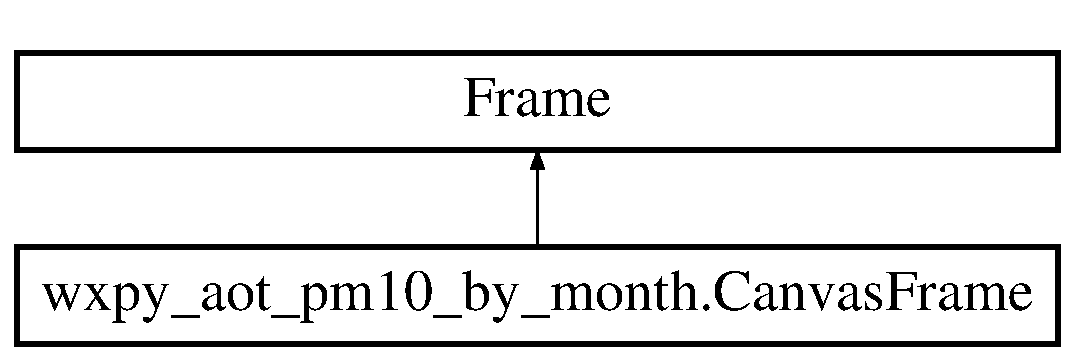
\includegraphics[height=2.000000cm]{classwxpy__aot__pm10__by__month_1_1_canvas_frame}
\end{center}
\end{figure}
\subsection*{Fonctions membres publiques}
\begin{DoxyCompactItemize}
\item 
def \hyperlink{classwxpy__aot__pm10__by__month_1_1_canvas_frame_a4de434fce1ba37499ae84d037c1c04d7}{\-\_\-\-\_\-init\-\_\-\-\_\-}
\item 
def \hyperlink{classwxpy__aot__pm10__by__month_1_1_canvas_frame_aecde9ea7e79178d7251a8ccfe771c25b}{Init\-Config}
\item 
def \hyperlink{classwxpy__aot__pm10__by__month_1_1_canvas_frame_a21fa0cfb666b8a2a8dad95a35fd05763}{unique}
\item 
def \hyperlink{classwxpy__aot__pm10__by__month_1_1_canvas_frame_acf3c1646918d532c1111be746de67029}{Prep\-Data}
\item 
def \hyperlink{classwxpy__aot__pm10__by__month_1_1_canvas_frame_ad95ddd57324d6de92c07a78dd02f08c0}{On\-Clicked}
\item 
def \hyperlink{classwxpy__aot__pm10__by__month_1_1_canvas_frame_a55dd7fc797814490cac2b8b484b91cd3}{On\-Paint}
\item 
def \hyperlink{classwxpy__aot__pm10__by__month_1_1_canvas_frame_a7a3d7557e440227e826e058e24a7dc34}{On\-Shell}
\item 
def \hyperlink{classwxpy__aot__pm10__by__month_1_1_canvas_frame_ae31f79a0d1731b8708bd3102598866f0}{On\-Filling}
\item 
def \hyperlink{classwxpy__aot__pm10__by__month_1_1_canvas_frame_af38f509f594e96042dd95bf948918633}{On\-Exit}
\item 
def \hyperlink{classwxpy__aot__pm10__by__month_1_1_canvas_frame_ab6d9e7f0f13c4fadaafb01d081e99a46}{On\-Options}
\end{DoxyCompactItemize}
\subsection*{Attributs publics}
\begin{DoxyCompactItemize}
\item 
\hyperlink{classwxpy__aot__pm10__by__month_1_1_canvas_frame_a1440364a6fda0aced69334348691db9a}{figure}
\item 
\hyperlink{classwxpy__aot__pm10__by__month_1_1_canvas_frame_abd0889715fef78b9d3e1b27804e6b5a7}{initdir}
\item 
\hyperlink{classwxpy__aot__pm10__by__month_1_1_canvas_frame_a2ec1012eb520bb1917248baec0526212}{canvas}
\item 
\hyperlink{classwxpy__aot__pm10__by__month_1_1_canvas_frame_aad49238c925c9414db374fae385040be}{sizer}
\item 
\hyperlink{classwxpy__aot__pm10__by__month_1_1_canvas_frame_a7eda9972e375d18a4c8d2ee6d7677a2a}{b\-Change\-Config}
\item 
\hyperlink{classwxpy__aot__pm10__by__month_1_1_canvas_frame_aac18d297677c222d00be26cad1876181}{toolbar}
\item 
\hyperlink{classwxpy__aot__pm10__by__month_1_1_canvas_frame_a131cdd35c70d8ea6e2ee9b587400d2ba}{Config}
\end{DoxyCompactItemize}


\subsection{Description détaillée}
\begin{DoxyVerb}Classe CanvasFrame \end{DoxyVerb}
 

\subsection{Documentation des constructeurs et destructeur}
\hypertarget{classwxpy__aot__pm10__by__month_1_1_canvas_frame_a4de434fce1ba37499ae84d037c1c04d7}{\index{wxpy\-\_\-aot\-\_\-pm10\-\_\-by\-\_\-month\-::\-Canvas\-Frame@{wxpy\-\_\-aot\-\_\-pm10\-\_\-by\-\_\-month\-::\-Canvas\-Frame}!\-\_\-\-\_\-init\-\_\-\-\_\-@{\-\_\-\-\_\-init\-\_\-\-\_\-}}
\index{\-\_\-\-\_\-init\-\_\-\-\_\-@{\-\_\-\-\_\-init\-\_\-\-\_\-}!wxpy_aot_pm10_by_month::CanvasFrame@{wxpy\-\_\-aot\-\_\-pm10\-\_\-by\-\_\-month\-::\-Canvas\-Frame}}
\subsubsection[{\-\_\-\-\_\-init\-\_\-\-\_\-}]{\setlength{\rightskip}{0pt plus 5cm}def wxpy\-\_\-aot\-\_\-pm10\-\_\-by\-\_\-month.\-Canvas\-Frame.\-\_\-\-\_\-init\-\_\-\-\_\- (
\begin{DoxyParamCaption}
\item[{}]{self}
\end{DoxyParamCaption}
)}}\label{classwxpy__aot__pm10__by__month_1_1_canvas_frame_a4de434fce1ba37499ae84d037c1c04d7}


\subsection{Documentation des fonctions membres}
\hypertarget{classwxpy__aot__pm10__by__month_1_1_canvas_frame_aecde9ea7e79178d7251a8ccfe771c25b}{\index{wxpy\-\_\-aot\-\_\-pm10\-\_\-by\-\_\-month\-::\-Canvas\-Frame@{wxpy\-\_\-aot\-\_\-pm10\-\_\-by\-\_\-month\-::\-Canvas\-Frame}!Init\-Config@{Init\-Config}}
\index{Init\-Config@{Init\-Config}!wxpy_aot_pm10_by_month::CanvasFrame@{wxpy\-\_\-aot\-\_\-pm10\-\_\-by\-\_\-month\-::\-Canvas\-Frame}}
\subsubsection[{Init\-Config}]{\setlength{\rightskip}{0pt plus 5cm}def wxpy\-\_\-aot\-\_\-pm10\-\_\-by\-\_\-month.\-Canvas\-Frame.\-Init\-Config (
\begin{DoxyParamCaption}
\item[{}]{self}
\end{DoxyParamCaption}
)}}\label{classwxpy__aot__pm10__by__month_1_1_canvas_frame_aecde9ea7e79178d7251a8ccfe771c25b}
\hypertarget{classwxpy__aot__pm10__by__month_1_1_canvas_frame_ad95ddd57324d6de92c07a78dd02f08c0}{\index{wxpy\-\_\-aot\-\_\-pm10\-\_\-by\-\_\-month\-::\-Canvas\-Frame@{wxpy\-\_\-aot\-\_\-pm10\-\_\-by\-\_\-month\-::\-Canvas\-Frame}!On\-Clicked@{On\-Clicked}}
\index{On\-Clicked@{On\-Clicked}!wxpy_aot_pm10_by_month::CanvasFrame@{wxpy\-\_\-aot\-\_\-pm10\-\_\-by\-\_\-month\-::\-Canvas\-Frame}}
\subsubsection[{On\-Clicked}]{\setlength{\rightskip}{0pt plus 5cm}def wxpy\-\_\-aot\-\_\-pm10\-\_\-by\-\_\-month.\-Canvas\-Frame.\-On\-Clicked (
\begin{DoxyParamCaption}
\item[{}]{self, }
\item[{}]{event}
\end{DoxyParamCaption}
)}}\label{classwxpy__aot__pm10__by__month_1_1_canvas_frame_ad95ddd57324d6de92c07a78dd02f08c0}
\hypertarget{classwxpy__aot__pm10__by__month_1_1_canvas_frame_af38f509f594e96042dd95bf948918633}{\index{wxpy\-\_\-aot\-\_\-pm10\-\_\-by\-\_\-month\-::\-Canvas\-Frame@{wxpy\-\_\-aot\-\_\-pm10\-\_\-by\-\_\-month\-::\-Canvas\-Frame}!On\-Exit@{On\-Exit}}
\index{On\-Exit@{On\-Exit}!wxpy_aot_pm10_by_month::CanvasFrame@{wxpy\-\_\-aot\-\_\-pm10\-\_\-by\-\_\-month\-::\-Canvas\-Frame}}
\subsubsection[{On\-Exit}]{\setlength{\rightskip}{0pt plus 5cm}def wxpy\-\_\-aot\-\_\-pm10\-\_\-by\-\_\-month.\-Canvas\-Frame.\-On\-Exit (
\begin{DoxyParamCaption}
\item[{}]{self, }
\item[{}]{event}
\end{DoxyParamCaption}
)}}\label{classwxpy__aot__pm10__by__month_1_1_canvas_frame_af38f509f594e96042dd95bf948918633}
\hypertarget{classwxpy__aot__pm10__by__month_1_1_canvas_frame_ae31f79a0d1731b8708bd3102598866f0}{\index{wxpy\-\_\-aot\-\_\-pm10\-\_\-by\-\_\-month\-::\-Canvas\-Frame@{wxpy\-\_\-aot\-\_\-pm10\-\_\-by\-\_\-month\-::\-Canvas\-Frame}!On\-Filling@{On\-Filling}}
\index{On\-Filling@{On\-Filling}!wxpy_aot_pm10_by_month::CanvasFrame@{wxpy\-\_\-aot\-\_\-pm10\-\_\-by\-\_\-month\-::\-Canvas\-Frame}}
\subsubsection[{On\-Filling}]{\setlength{\rightskip}{0pt plus 5cm}def wxpy\-\_\-aot\-\_\-pm10\-\_\-by\-\_\-month.\-Canvas\-Frame.\-On\-Filling (
\begin{DoxyParamCaption}
\item[{}]{self, }
\item[{}]{event}
\end{DoxyParamCaption}
)}}\label{classwxpy__aot__pm10__by__month_1_1_canvas_frame_ae31f79a0d1731b8708bd3102598866f0}
\begin{DoxyVerb}Browser pycrust \end{DoxyVerb}
 \hypertarget{classwxpy__aot__pm10__by__month_1_1_canvas_frame_ab6d9e7f0f13c4fadaafb01d081e99a46}{\index{wxpy\-\_\-aot\-\_\-pm10\-\_\-by\-\_\-month\-::\-Canvas\-Frame@{wxpy\-\_\-aot\-\_\-pm10\-\_\-by\-\_\-month\-::\-Canvas\-Frame}!On\-Options@{On\-Options}}
\index{On\-Options@{On\-Options}!wxpy_aot_pm10_by_month::CanvasFrame@{wxpy\-\_\-aot\-\_\-pm10\-\_\-by\-\_\-month\-::\-Canvas\-Frame}}
\subsubsection[{On\-Options}]{\setlength{\rightskip}{0pt plus 5cm}def wxpy\-\_\-aot\-\_\-pm10\-\_\-by\-\_\-month.\-Canvas\-Frame.\-On\-Options (
\begin{DoxyParamCaption}
\item[{}]{self, }
\item[{}]{event}
\end{DoxyParamCaption}
)}}\label{classwxpy__aot__pm10__by__month_1_1_canvas_frame_ab6d9e7f0f13c4fadaafb01d081e99a46}
\begin{DoxyVerb}Parameters Dialog Handler \end{DoxyVerb}
 \hypertarget{classwxpy__aot__pm10__by__month_1_1_canvas_frame_a55dd7fc797814490cac2b8b484b91cd3}{\index{wxpy\-\_\-aot\-\_\-pm10\-\_\-by\-\_\-month\-::\-Canvas\-Frame@{wxpy\-\_\-aot\-\_\-pm10\-\_\-by\-\_\-month\-::\-Canvas\-Frame}!On\-Paint@{On\-Paint}}
\index{On\-Paint@{On\-Paint}!wxpy_aot_pm10_by_month::CanvasFrame@{wxpy\-\_\-aot\-\_\-pm10\-\_\-by\-\_\-month\-::\-Canvas\-Frame}}
\subsubsection[{On\-Paint}]{\setlength{\rightskip}{0pt plus 5cm}def wxpy\-\_\-aot\-\_\-pm10\-\_\-by\-\_\-month.\-Canvas\-Frame.\-On\-Paint (
\begin{DoxyParamCaption}
\item[{}]{self, }
\item[{}]{event}
\end{DoxyParamCaption}
)}}\label{classwxpy__aot__pm10__by__month_1_1_canvas_frame_a55dd7fc797814490cac2b8b484b91cd3}
\hypertarget{classwxpy__aot__pm10__by__month_1_1_canvas_frame_a7a3d7557e440227e826e058e24a7dc34}{\index{wxpy\-\_\-aot\-\_\-pm10\-\_\-by\-\_\-month\-::\-Canvas\-Frame@{wxpy\-\_\-aot\-\_\-pm10\-\_\-by\-\_\-month\-::\-Canvas\-Frame}!On\-Shell@{On\-Shell}}
\index{On\-Shell@{On\-Shell}!wxpy_aot_pm10_by_month::CanvasFrame@{wxpy\-\_\-aot\-\_\-pm10\-\_\-by\-\_\-month\-::\-Canvas\-Frame}}
\subsubsection[{On\-Shell}]{\setlength{\rightskip}{0pt plus 5cm}def wxpy\-\_\-aot\-\_\-pm10\-\_\-by\-\_\-month.\-Canvas\-Frame.\-On\-Shell (
\begin{DoxyParamCaption}
\item[{}]{self, }
\item[{}]{event}
\end{DoxyParamCaption}
)}}\label{classwxpy__aot__pm10__by__month_1_1_canvas_frame_a7a3d7557e440227e826e058e24a7dc34}
\begin{DoxyVerb}Shell pycrust \end{DoxyVerb}
 \hypertarget{classwxpy__aot__pm10__by__month_1_1_canvas_frame_acf3c1646918d532c1111be746de67029}{\index{wxpy\-\_\-aot\-\_\-pm10\-\_\-by\-\_\-month\-::\-Canvas\-Frame@{wxpy\-\_\-aot\-\_\-pm10\-\_\-by\-\_\-month\-::\-Canvas\-Frame}!Prep\-Data@{Prep\-Data}}
\index{Prep\-Data@{Prep\-Data}!wxpy_aot_pm10_by_month::CanvasFrame@{wxpy\-\_\-aot\-\_\-pm10\-\_\-by\-\_\-month\-::\-Canvas\-Frame}}
\subsubsection[{Prep\-Data}]{\setlength{\rightskip}{0pt plus 5cm}def wxpy\-\_\-aot\-\_\-pm10\-\_\-by\-\_\-month.\-Canvas\-Frame.\-Prep\-Data (
\begin{DoxyParamCaption}
\item[{}]{self}
\end{DoxyParamCaption}
)}}\label{classwxpy__aot__pm10__by__month_1_1_canvas_frame_acf3c1646918d532c1111be746de67029}
\begin{DoxyVerb}Prepare data before plotting \end{DoxyVerb}
 \hypertarget{classwxpy__aot__pm10__by__month_1_1_canvas_frame_a21fa0cfb666b8a2a8dad95a35fd05763}{\index{wxpy\-\_\-aot\-\_\-pm10\-\_\-by\-\_\-month\-::\-Canvas\-Frame@{wxpy\-\_\-aot\-\_\-pm10\-\_\-by\-\_\-month\-::\-Canvas\-Frame}!unique@{unique}}
\index{unique@{unique}!wxpy_aot_pm10_by_month::CanvasFrame@{wxpy\-\_\-aot\-\_\-pm10\-\_\-by\-\_\-month\-::\-Canvas\-Frame}}
\subsubsection[{unique}]{\setlength{\rightskip}{0pt plus 5cm}def wxpy\-\_\-aot\-\_\-pm10\-\_\-by\-\_\-month.\-Canvas\-Frame.\-unique (
\begin{DoxyParamCaption}
\item[{}]{self, }
\item[{}]{a}
\end{DoxyParamCaption}
)}}\label{classwxpy__aot__pm10__by__month_1_1_canvas_frame_a21fa0cfb666b8a2a8dad95a35fd05763}
\begin{DoxyVerb}Renvoie un vecteur contenant les valeurs uniques d'un vecteur  \end{DoxyVerb}
 

\subsection{Documentation des données membres}
\hypertarget{classwxpy__aot__pm10__by__month_1_1_canvas_frame_a7eda9972e375d18a4c8d2ee6d7677a2a}{\index{wxpy\-\_\-aot\-\_\-pm10\-\_\-by\-\_\-month\-::\-Canvas\-Frame@{wxpy\-\_\-aot\-\_\-pm10\-\_\-by\-\_\-month\-::\-Canvas\-Frame}!b\-Change\-Config@{b\-Change\-Config}}
\index{b\-Change\-Config@{b\-Change\-Config}!wxpy_aot_pm10_by_month::CanvasFrame@{wxpy\-\_\-aot\-\_\-pm10\-\_\-by\-\_\-month\-::\-Canvas\-Frame}}
\subsubsection[{b\-Change\-Config}]{\setlength{\rightskip}{0pt plus 5cm}wxpy\-\_\-aot\-\_\-pm10\-\_\-by\-\_\-month.\-Canvas\-Frame.\-b\-Change\-Config}}\label{classwxpy__aot__pm10__by__month_1_1_canvas_frame_a7eda9972e375d18a4c8d2ee6d7677a2a}
\hypertarget{classwxpy__aot__pm10__by__month_1_1_canvas_frame_a2ec1012eb520bb1917248baec0526212}{\index{wxpy\-\_\-aot\-\_\-pm10\-\_\-by\-\_\-month\-::\-Canvas\-Frame@{wxpy\-\_\-aot\-\_\-pm10\-\_\-by\-\_\-month\-::\-Canvas\-Frame}!canvas@{canvas}}
\index{canvas@{canvas}!wxpy_aot_pm10_by_month::CanvasFrame@{wxpy\-\_\-aot\-\_\-pm10\-\_\-by\-\_\-month\-::\-Canvas\-Frame}}
\subsubsection[{canvas}]{\setlength{\rightskip}{0pt plus 5cm}wxpy\-\_\-aot\-\_\-pm10\-\_\-by\-\_\-month.\-Canvas\-Frame.\-canvas}}\label{classwxpy__aot__pm10__by__month_1_1_canvas_frame_a2ec1012eb520bb1917248baec0526212}
\hypertarget{classwxpy__aot__pm10__by__month_1_1_canvas_frame_a131cdd35c70d8ea6e2ee9b587400d2ba}{\index{wxpy\-\_\-aot\-\_\-pm10\-\_\-by\-\_\-month\-::\-Canvas\-Frame@{wxpy\-\_\-aot\-\_\-pm10\-\_\-by\-\_\-month\-::\-Canvas\-Frame}!Config@{Config}}
\index{Config@{Config}!wxpy_aot_pm10_by_month::CanvasFrame@{wxpy\-\_\-aot\-\_\-pm10\-\_\-by\-\_\-month\-::\-Canvas\-Frame}}
\subsubsection[{Config}]{\setlength{\rightskip}{0pt plus 5cm}wxpy\-\_\-aot\-\_\-pm10\-\_\-by\-\_\-month.\-Canvas\-Frame.\-Config}}\label{classwxpy__aot__pm10__by__month_1_1_canvas_frame_a131cdd35c70d8ea6e2ee9b587400d2ba}
\hypertarget{classwxpy__aot__pm10__by__month_1_1_canvas_frame_a1440364a6fda0aced69334348691db9a}{\index{wxpy\-\_\-aot\-\_\-pm10\-\_\-by\-\_\-month\-::\-Canvas\-Frame@{wxpy\-\_\-aot\-\_\-pm10\-\_\-by\-\_\-month\-::\-Canvas\-Frame}!figure@{figure}}
\index{figure@{figure}!wxpy_aot_pm10_by_month::CanvasFrame@{wxpy\-\_\-aot\-\_\-pm10\-\_\-by\-\_\-month\-::\-Canvas\-Frame}}
\subsubsection[{figure}]{\setlength{\rightskip}{0pt plus 5cm}wxpy\-\_\-aot\-\_\-pm10\-\_\-by\-\_\-month.\-Canvas\-Frame.\-figure}}\label{classwxpy__aot__pm10__by__month_1_1_canvas_frame_a1440364a6fda0aced69334348691db9a}
\hypertarget{classwxpy__aot__pm10__by__month_1_1_canvas_frame_abd0889715fef78b9d3e1b27804e6b5a7}{\index{wxpy\-\_\-aot\-\_\-pm10\-\_\-by\-\_\-month\-::\-Canvas\-Frame@{wxpy\-\_\-aot\-\_\-pm10\-\_\-by\-\_\-month\-::\-Canvas\-Frame}!initdir@{initdir}}
\index{initdir@{initdir}!wxpy_aot_pm10_by_month::CanvasFrame@{wxpy\-\_\-aot\-\_\-pm10\-\_\-by\-\_\-month\-::\-Canvas\-Frame}}
\subsubsection[{initdir}]{\setlength{\rightskip}{0pt plus 5cm}wxpy\-\_\-aot\-\_\-pm10\-\_\-by\-\_\-month.\-Canvas\-Frame.\-initdir}}\label{classwxpy__aot__pm10__by__month_1_1_canvas_frame_abd0889715fef78b9d3e1b27804e6b5a7}
\hypertarget{classwxpy__aot__pm10__by__month_1_1_canvas_frame_aad49238c925c9414db374fae385040be}{\index{wxpy\-\_\-aot\-\_\-pm10\-\_\-by\-\_\-month\-::\-Canvas\-Frame@{wxpy\-\_\-aot\-\_\-pm10\-\_\-by\-\_\-month\-::\-Canvas\-Frame}!sizer@{sizer}}
\index{sizer@{sizer}!wxpy_aot_pm10_by_month::CanvasFrame@{wxpy\-\_\-aot\-\_\-pm10\-\_\-by\-\_\-month\-::\-Canvas\-Frame}}
\subsubsection[{sizer}]{\setlength{\rightskip}{0pt plus 5cm}wxpy\-\_\-aot\-\_\-pm10\-\_\-by\-\_\-month.\-Canvas\-Frame.\-sizer}}\label{classwxpy__aot__pm10__by__month_1_1_canvas_frame_aad49238c925c9414db374fae385040be}
\hypertarget{classwxpy__aot__pm10__by__month_1_1_canvas_frame_aac18d297677c222d00be26cad1876181}{\index{wxpy\-\_\-aot\-\_\-pm10\-\_\-by\-\_\-month\-::\-Canvas\-Frame@{wxpy\-\_\-aot\-\_\-pm10\-\_\-by\-\_\-month\-::\-Canvas\-Frame}!toolbar@{toolbar}}
\index{toolbar@{toolbar}!wxpy_aot_pm10_by_month::CanvasFrame@{wxpy\-\_\-aot\-\_\-pm10\-\_\-by\-\_\-month\-::\-Canvas\-Frame}}
\subsubsection[{toolbar}]{\setlength{\rightskip}{0pt plus 5cm}wxpy\-\_\-aot\-\_\-pm10\-\_\-by\-\_\-month.\-Canvas\-Frame.\-toolbar}}\label{classwxpy__aot__pm10__by__month_1_1_canvas_frame_aac18d297677c222d00be26cad1876181}


La documentation de cette classe a été générée à partir du fichier suivant \-:\begin{DoxyCompactItemize}
\item 
\hyperlink{wxpy__aot__pm10__by__month_8py}{wxpy\-\_\-aot\-\_\-pm10\-\_\-by\-\_\-month.\-py}\end{DoxyCompactItemize}

\hypertarget{classdatefromday_1_1datefromday}{\section{Référence de la classe datefromday.\-datefromday}
\label{classdatefromday_1_1datefromday}\index{datefromday.\-datefromday@{datefromday.\-datefromday}}
}
\subsection*{Fonctions membres publiques}
\begin{DoxyCompactItemize}
\item 
def \hyperlink{classdatefromday_1_1datefromday_aa54010cbbfea33d558a09ee90b3b5306}{\-\_\-\-\_\-init\-\_\-\-\_\-}
\item 
def \hyperlink{classdatefromday_1_1datefromday_ad0f9a3b9f4fdf0d8c005a19772498c95}{get\-String\-Year}
\item 
def \hyperlink{classdatefromday_1_1datefromday_a6e85aa539dc264d7fb2d3b37788bce7b}{get\-String\-Month}
\item 
def \hyperlink{classdatefromday_1_1datefromday_a8e7d4bebfddba74880919c58d5633d15}{get\-String\-Day}
\item 
def \hyperlink{classdatefromday_1_1datefromday_a8c72473924a49d1d975edb18f73d877b}{get\-\_\-day\-\_\-of\-\_\-week}
\item 
def \hyperlink{classdatefromday_1_1datefromday_a2a686f37ac2d71546d926c2188823b1c}{get\-Array}
\item 
def \hyperlink{classdatefromday_1_1datefromday_a2d0334466197d676daa1c25d61b529c2}{get\-String}
\end{DoxyCompactItemize}
\subsection*{Attributs publics}
\begin{DoxyCompactItemize}
\item 
\hyperlink{classdatefromday_1_1datefromday_a705eb03010097a53a5813aedb360ee30}{year}
\item 
\hyperlink{classdatefromday_1_1datefromday_a4f9694b8f18756495c1d79fdb6967350}{njour}
\item 
\hyperlink{classdatefromday_1_1datefromday_a82528e422e7b12f870894efafa9677db}{resday}
\item 
\hyperlink{classdatefromday_1_1datefromday_ac29c28e89d058d5a9c175c74ba604e8d}{resmonth}
\end{DoxyCompactItemize}
\subsection*{Attributs publics statiques}
\begin{DoxyCompactItemize}
\item 
tuple \hyperlink{classdatefromday_1_1datefromday_aea92e2e72937fab296b235453854f0c8}{nweekday} = datetime.\-date(y,m,d)
\end{DoxyCompactItemize}


\subsection{Documentation des constructeurs et destructeur}
\hypertarget{classdatefromday_1_1datefromday_aa54010cbbfea33d558a09ee90b3b5306}{\index{datefromday\-::datefromday@{datefromday\-::datefromday}!\-\_\-\-\_\-init\-\_\-\-\_\-@{\-\_\-\-\_\-init\-\_\-\-\_\-}}
\index{\-\_\-\-\_\-init\-\_\-\-\_\-@{\-\_\-\-\_\-init\-\_\-\-\_\-}!datefromday::datefromday@{datefromday\-::datefromday}}
\subsubsection[{\-\_\-\-\_\-init\-\_\-\-\_\-}]{\setlength{\rightskip}{0pt plus 5cm}def datefromday.\-datefromday.\-\_\-\-\_\-init\-\_\-\-\_\- (
\begin{DoxyParamCaption}
\item[{}]{self, }
\item[{}]{year, }
\item[{}]{njour}
\end{DoxyParamCaption}
)}}\label{classdatefromday_1_1datefromday_aa54010cbbfea33d558a09ee90b3b5306}


\subsection{Documentation des fonctions membres}
\hypertarget{classdatefromday_1_1datefromday_a8c72473924a49d1d975edb18f73d877b}{\index{datefromday\-::datefromday@{datefromday\-::datefromday}!get\-\_\-day\-\_\-of\-\_\-week@{get\-\_\-day\-\_\-of\-\_\-week}}
\index{get\-\_\-day\-\_\-of\-\_\-week@{get\-\_\-day\-\_\-of\-\_\-week}!datefromday::datefromday@{datefromday\-::datefromday}}
\subsubsection[{get\-\_\-day\-\_\-of\-\_\-week}]{\setlength{\rightskip}{0pt plus 5cm}def datefromday.\-datefromday.\-get\-\_\-day\-\_\-of\-\_\-week (
\begin{DoxyParamCaption}
\item[{}]{self}
\end{DoxyParamCaption}
)}}\label{classdatefromday_1_1datefromday_a8c72473924a49d1d975edb18f73d877b}
\hypertarget{classdatefromday_1_1datefromday_a2a686f37ac2d71546d926c2188823b1c}{\index{datefromday\-::datefromday@{datefromday\-::datefromday}!get\-Array@{get\-Array}}
\index{get\-Array@{get\-Array}!datefromday::datefromday@{datefromday\-::datefromday}}
\subsubsection[{get\-Array}]{\setlength{\rightskip}{0pt plus 5cm}def datefromday.\-datefromday.\-get\-Array (
\begin{DoxyParamCaption}
\item[{}]{self}
\end{DoxyParamCaption}
)}}\label{classdatefromday_1_1datefromday_a2a686f37ac2d71546d926c2188823b1c}
\hypertarget{classdatefromday_1_1datefromday_a2d0334466197d676daa1c25d61b529c2}{\index{datefromday\-::datefromday@{datefromday\-::datefromday}!get\-String@{get\-String}}
\index{get\-String@{get\-String}!datefromday::datefromday@{datefromday\-::datefromday}}
\subsubsection[{get\-String}]{\setlength{\rightskip}{0pt plus 5cm}def datefromday.\-datefromday.\-get\-String (
\begin{DoxyParamCaption}
\item[{}]{self}
\end{DoxyParamCaption}
)}}\label{classdatefromday_1_1datefromday_a2d0334466197d676daa1c25d61b529c2}
\hypertarget{classdatefromday_1_1datefromday_a8e7d4bebfddba74880919c58d5633d15}{\index{datefromday\-::datefromday@{datefromday\-::datefromday}!get\-String\-Day@{get\-String\-Day}}
\index{get\-String\-Day@{get\-String\-Day}!datefromday::datefromday@{datefromday\-::datefromday}}
\subsubsection[{get\-String\-Day}]{\setlength{\rightskip}{0pt plus 5cm}def datefromday.\-datefromday.\-get\-String\-Day (
\begin{DoxyParamCaption}
\item[{}]{self}
\end{DoxyParamCaption}
)}}\label{classdatefromday_1_1datefromday_a8e7d4bebfddba74880919c58d5633d15}
\hypertarget{classdatefromday_1_1datefromday_a6e85aa539dc264d7fb2d3b37788bce7b}{\index{datefromday\-::datefromday@{datefromday\-::datefromday}!get\-String\-Month@{get\-String\-Month}}
\index{get\-String\-Month@{get\-String\-Month}!datefromday::datefromday@{datefromday\-::datefromday}}
\subsubsection[{get\-String\-Month}]{\setlength{\rightskip}{0pt plus 5cm}def datefromday.\-datefromday.\-get\-String\-Month (
\begin{DoxyParamCaption}
\item[{}]{self}
\end{DoxyParamCaption}
)}}\label{classdatefromday_1_1datefromday_a6e85aa539dc264d7fb2d3b37788bce7b}
\hypertarget{classdatefromday_1_1datefromday_ad0f9a3b9f4fdf0d8c005a19772498c95}{\index{datefromday\-::datefromday@{datefromday\-::datefromday}!get\-String\-Year@{get\-String\-Year}}
\index{get\-String\-Year@{get\-String\-Year}!datefromday::datefromday@{datefromday\-::datefromday}}
\subsubsection[{get\-String\-Year}]{\setlength{\rightskip}{0pt plus 5cm}def datefromday.\-datefromday.\-get\-String\-Year (
\begin{DoxyParamCaption}
\item[{}]{self}
\end{DoxyParamCaption}
)}}\label{classdatefromday_1_1datefromday_ad0f9a3b9f4fdf0d8c005a19772498c95}


\subsection{Documentation des données membres}
\hypertarget{classdatefromday_1_1datefromday_a4f9694b8f18756495c1d79fdb6967350}{\index{datefromday\-::datefromday@{datefromday\-::datefromday}!njour@{njour}}
\index{njour@{njour}!datefromday::datefromday@{datefromday\-::datefromday}}
\subsubsection[{njour}]{\setlength{\rightskip}{0pt plus 5cm}datefromday.\-datefromday.\-njour}}\label{classdatefromday_1_1datefromday_a4f9694b8f18756495c1d79fdb6967350}
\hypertarget{classdatefromday_1_1datefromday_aea92e2e72937fab296b235453854f0c8}{\index{datefromday\-::datefromday@{datefromday\-::datefromday}!nweekday@{nweekday}}
\index{nweekday@{nweekday}!datefromday::datefromday@{datefromday\-::datefromday}}
\subsubsection[{nweekday}]{\setlength{\rightskip}{0pt plus 5cm}tuple datefromday.\-datefromday.\-nweekday = datetime.\-date(y,m,d)\hspace{0.3cm}{\ttfamily [static]}}}\label{classdatefromday_1_1datefromday_aea92e2e72937fab296b235453854f0c8}
\hypertarget{classdatefromday_1_1datefromday_a82528e422e7b12f870894efafa9677db}{\index{datefromday\-::datefromday@{datefromday\-::datefromday}!resday@{resday}}
\index{resday@{resday}!datefromday::datefromday@{datefromday\-::datefromday}}
\subsubsection[{resday}]{\setlength{\rightskip}{0pt plus 5cm}datefromday.\-datefromday.\-resday}}\label{classdatefromday_1_1datefromday_a82528e422e7b12f870894efafa9677db}
\hypertarget{classdatefromday_1_1datefromday_ac29c28e89d058d5a9c175c74ba604e8d}{\index{datefromday\-::datefromday@{datefromday\-::datefromday}!resmonth@{resmonth}}
\index{resmonth@{resmonth}!datefromday::datefromday@{datefromday\-::datefromday}}
\subsubsection[{resmonth}]{\setlength{\rightskip}{0pt plus 5cm}datefromday.\-datefromday.\-resmonth}}\label{classdatefromday_1_1datefromday_ac29c28e89d058d5a9c175c74ba604e8d}
\hypertarget{classdatefromday_1_1datefromday_a705eb03010097a53a5813aedb360ee30}{\index{datefromday\-::datefromday@{datefromday\-::datefromday}!year@{year}}
\index{year@{year}!datefromday::datefromday@{datefromday\-::datefromday}}
\subsubsection[{year}]{\setlength{\rightskip}{0pt plus 5cm}datefromday.\-datefromday.\-year}}\label{classdatefromday_1_1datefromday_a705eb03010097a53a5813aedb360ee30}


La documentation de cette classe a été générée à partir du fichier suivant \-:\begin{DoxyCompactItemize}
\item 
\hyperlink{datefromday_8py}{datefromday.\-py}\end{DoxyCompactItemize}

\hypertarget{classdayfromdate_1_1dayfromdate}{\section{Référence de la classe dayfromdate.\-dayfromdate}
\label{classdayfromdate_1_1dayfromdate}\index{dayfromdate.\-dayfromdate@{dayfromdate.\-dayfromdate}}
}
\subsection*{Fonctions membres publiques}
\begin{DoxyCompactItemize}
\item 
def \hyperlink{classdayfromdate_1_1dayfromdate_a50f63524775f9f96d245010fc71539ca}{\-\_\-\-\_\-init\-\_\-\-\_\-}
\item 
def \hyperlink{classdayfromdate_1_1dayfromdate_a30a04099233975c04ba24adcb89b0e00}{getn\-Day}
\end{DoxyCompactItemize}
\subsection*{Attributs publics}
\begin{DoxyCompactItemize}
\item 
\hyperlink{classdayfromdate_1_1dayfromdate_a706a784e42cee38a42d850296c48edba}{date}
\end{DoxyCompactItemize}


\subsection{Description détaillée}
\begin{DoxyVerb}Trouver le num�ro du jour � partir de la date en clair \end{DoxyVerb}
 

\subsection{Documentation des constructeurs et destructeur}
\hypertarget{classdayfromdate_1_1dayfromdate_a50f63524775f9f96d245010fc71539ca}{\index{dayfromdate\-::dayfromdate@{dayfromdate\-::dayfromdate}!\-\_\-\-\_\-init\-\_\-\-\_\-@{\-\_\-\-\_\-init\-\_\-\-\_\-}}
\index{\-\_\-\-\_\-init\-\_\-\-\_\-@{\-\_\-\-\_\-init\-\_\-\-\_\-}!dayfromdate::dayfromdate@{dayfromdate\-::dayfromdate}}
\subsubsection[{\-\_\-\-\_\-init\-\_\-\-\_\-}]{\setlength{\rightskip}{0pt plus 5cm}def dayfromdate.\-dayfromdate.\-\_\-\-\_\-init\-\_\-\-\_\- (
\begin{DoxyParamCaption}
\item[{}]{self, }
\item[{}]{year, }
\item[{}]{month, }
\item[{}]{day}
\end{DoxyParamCaption}
)}}\label{classdayfromdate_1_1dayfromdate_a50f63524775f9f96d245010fc71539ca}
\begin{DoxyVerb}Get day number from date \end{DoxyVerb}
 

\subsection{Documentation des fonctions membres}
\hypertarget{classdayfromdate_1_1dayfromdate_a30a04099233975c04ba24adcb89b0e00}{\index{dayfromdate\-::dayfromdate@{dayfromdate\-::dayfromdate}!getn\-Day@{getn\-Day}}
\index{getn\-Day@{getn\-Day}!dayfromdate::dayfromdate@{dayfromdate\-::dayfromdate}}
\subsubsection[{getn\-Day}]{\setlength{\rightskip}{0pt plus 5cm}def dayfromdate.\-dayfromdate.\-getn\-Day (
\begin{DoxyParamCaption}
\item[{}]{self}
\end{DoxyParamCaption}
)}}\label{classdayfromdate_1_1dayfromdate_a30a04099233975c04ba24adcb89b0e00}
\begin{DoxyVerb}R�ucp�rer le num�ro du jour \end{DoxyVerb}
 

\subsection{Documentation des données membres}
\hypertarget{classdayfromdate_1_1dayfromdate_a706a784e42cee38a42d850296c48edba}{\index{dayfromdate\-::dayfromdate@{dayfromdate\-::dayfromdate}!date@{date}}
\index{date@{date}!dayfromdate::dayfromdate@{dayfromdate\-::dayfromdate}}
\subsubsection[{date}]{\setlength{\rightskip}{0pt plus 5cm}dayfromdate.\-dayfromdate.\-date}}\label{classdayfromdate_1_1dayfromdate_a706a784e42cee38a42d850296c48edba}


La documentation de cette classe a été générée à partir du fichier suivant \-:\begin{DoxyCompactItemize}
\item 
\hyperlink{dayfromdate_8py}{dayfromdate.\-py}\end{DoxyCompactItemize}

\hypertarget{classwxpy__aot__pm10__by__month_1_1_my_navigation_toolbar}{\section{Référence de la classe wxpy\-\_\-aot\-\_\-pm10\-\_\-by\-\_\-month.\-My\-Navigation\-Toolbar}
\label{classwxpy__aot__pm10__by__month_1_1_my_navigation_toolbar}\index{wxpy\-\_\-aot\-\_\-pm10\-\_\-by\-\_\-month.\-My\-Navigation\-Toolbar@{wxpy\-\_\-aot\-\_\-pm10\-\_\-by\-\_\-month.\-My\-Navigation\-Toolbar}}
}
Graphe d'héritage de wxpy\-\_\-aot\-\_\-pm10\-\_\-by\-\_\-month.\-My\-Navigation\-Toolbar\-:\begin{figure}[H]
\begin{center}
\leavevmode
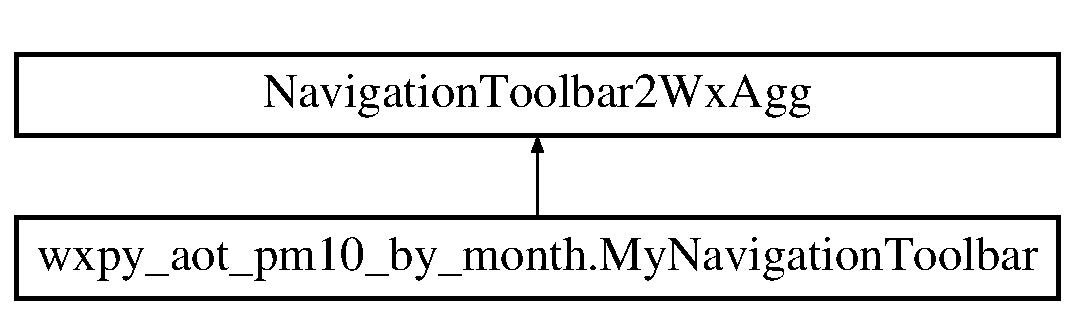
\includegraphics[height=2.000000cm]{classwxpy__aot__pm10__by__month_1_1_my_navigation_toolbar}
\end{center}
\end{figure}
\subsection*{Fonctions membres publiques}
\begin{DoxyCompactItemize}
\item 
def \hyperlink{classwxpy__aot__pm10__by__month_1_1_my_navigation_toolbar_aef2f22a8eef273ab8e865c165c2b95a0}{\-\_\-\-\_\-init\-\_\-\-\_\-}
\item 
def \hyperlink{classwxpy__aot__pm10__by__month_1_1_my_navigation_toolbar_a32de3683254bb5e8b545c0a19550d39f}{initmois}
\item 
def \hyperlink{classwxpy__aot__pm10__by__month_1_1_my_navigation_toolbar_adaec7999dbd73e0babab1cc3c859c494}{get\-\_\-jour\-\_\-en\-\_\-clair}
\item 
def \hyperlink{classwxpy__aot__pm10__by__month_1_1_my_navigation_toolbar_a09695342601aaa000e988fc0be21ee17}{get\-\_\-mois\-\_\-en\-\_\-clair}
\item 
def \hyperlink{classwxpy__aot__pm10__by__month_1_1_my_navigation_toolbar_a1c683ed5a6916c1ba14d0a6d46002996}{get\-\_\-string\-\_\-day}
\item 
def \hyperlink{classwxpy__aot__pm10__by__month_1_1_my_navigation_toolbar_a176af92bff6575b515f73aeeecf3fa8e}{getvg0n}
\item 
def \hyperlink{classwxpy__aot__pm10__by__month_1_1_my_navigation_toolbar_a7e5235a5fb7707a2fae10022843b0336}{getvg0\-\_\-month}
\item 
def \hyperlink{classwxpy__aot__pm10__by__month_1_1_my_navigation_toolbar_a03c4d636b0b3a94cb5cf4e2a0f695cb7}{getvg0\-\_\-2\-\_\-month}
\item 
def \hyperlink{classwxpy__aot__pm10__by__month_1_1_my_navigation_toolbar_afe72b37295f17b4cdeab855cec2e725d}{draw}
\item 
def \hyperlink{classwxpy__aot__pm10__by__month_1_1_my_navigation_toolbar_a2a56e0bf79d60d48c35d9964562334e7}{save}
\end{DoxyCompactItemize}
\subsection*{Attributs publics}
\begin{DoxyCompactItemize}
\item 
\hyperlink{classwxpy__aot__pm10__by__month_1_1_my_navigation_toolbar_af80aed2f935326d558930bc9cd459bd1}{canvas}
\item 
\hyperlink{classwxpy__aot__pm10__by__month_1_1_my_navigation_toolbar_a6253f661597cbdb59a97d0dac9be0e8b}{O\-N\-\_\-\-P\-R\-E\-V\-I\-O\-U\-S}
\item 
\hyperlink{classwxpy__aot__pm10__by__month_1_1_my_navigation_toolbar_adbfd6cc1963d767f3a3b18082644dea7}{O\-N\-\_\-\-N\-E\-X\-T}
\item 
\hyperlink{classwxpy__aot__pm10__by__month_1_1_my_navigation_toolbar_ae8f2c4519688c382469d0f31aa3384ea}{O\-N\-\_\-\-L\-I\-S\-T\-E}
\item 
\hyperlink{classwxpy__aot__pm10__by__month_1_1_my_navigation_toolbar_afcbec75416ece51149cfbd212a2f2a4e}{nmois}
\end{DoxyCompactItemize}
\subsection*{Attributs publics statiques}
\begin{DoxyCompactItemize}
\item 
tuple \hyperlink{classwxpy__aot__pm10__by__month_1_1_my_navigation_toolbar_a6ef4dc9c22340649bb209aa695adb07f}{keys\-\_\-sort} = self.\-dirmois.\-keys()
\item 
tuple \hyperlink{classwxpy__aot__pm10__by__month_1_1_my_navigation_toolbar_aa7ad170be2c3289e6f20bf13ebd44ea7}{nweekday} = datefromday(2009,njour)
\item 
tuple \hyperlink{classwxpy__aot__pm10__by__month_1_1_my_navigation_toolbar_ac229be2055516da3111b4b9885ae7535}{dlg}
\item 
int \hyperlink{classwxpy__aot__pm10__by__month_1_1_my_navigation_toolbar_a5b397c90bed2b8778deb36693e2a6db8}{indice} = 0
\item 
list \hyperlink{classwxpy__aot__pm10__by__month_1_1_my_navigation_toolbar_accd501ca8c996cb9e132d88ce1359941}{ax} = self.\-canvas.\-figure.\-axes\mbox{[}0\mbox{]}
\item 
tuple \hyperlink{classwxpy__aot__pm10__by__month_1_1_my_navigation_toolbar_afc958c6e6b8440395b4145f1258c5788}{vg0n} = self.\-getvg0\-\_\-month(self.\-nmois)
\item 
tuple \hyperlink{classwxpy__aot__pm10__by__month_1_1_my_navigation_toolbar_ad166dec3c81bf8b2ed37ac9a7dfbd81a}{vg0n\-\_\-2} = self.\-getvg0\-\_\-2\-\_\-month(self.\-nmois)
\item 
int \hyperlink{classwxpy__aot__pm10__by__month_1_1_my_navigation_toolbar_ac11e40e5da753c43e7745e8fa4f16828}{markersize} = 12
\end{DoxyCompactItemize}


\subsection{Description détaillée}
\begin{DoxyVerb}Extend the default wx toolbar with your own event handlers
\end{DoxyVerb}
 

\subsection{Documentation des constructeurs et destructeur}
\hypertarget{classwxpy__aot__pm10__by__month_1_1_my_navigation_toolbar_aef2f22a8eef273ab8e865c165c2b95a0}{\index{wxpy\-\_\-aot\-\_\-pm10\-\_\-by\-\_\-month\-::\-My\-Navigation\-Toolbar@{wxpy\-\_\-aot\-\_\-pm10\-\_\-by\-\_\-month\-::\-My\-Navigation\-Toolbar}!\-\_\-\-\_\-init\-\_\-\-\_\-@{\-\_\-\-\_\-init\-\_\-\-\_\-}}
\index{\-\_\-\-\_\-init\-\_\-\-\_\-@{\-\_\-\-\_\-init\-\_\-\-\_\-}!wxpy_aot_pm10_by_month::MyNavigationToolbar@{wxpy\-\_\-aot\-\_\-pm10\-\_\-by\-\_\-month\-::\-My\-Navigation\-Toolbar}}
\subsubsection[{\-\_\-\-\_\-init\-\_\-\-\_\-}]{\setlength{\rightskip}{0pt plus 5cm}def wxpy\-\_\-aot\-\_\-pm10\-\_\-by\-\_\-month.\-My\-Navigation\-Toolbar.\-\_\-\-\_\-init\-\_\-\-\_\- (
\begin{DoxyParamCaption}
\item[{}]{self, }
\item[{}]{canvas, }
\item[{}]{cankill}
\end{DoxyParamCaption}
)}}\label{classwxpy__aot__pm10__by__month_1_1_my_navigation_toolbar_aef2f22a8eef273ab8e865c165c2b95a0}


\subsection{Documentation des fonctions membres}
\hypertarget{classwxpy__aot__pm10__by__month_1_1_my_navigation_toolbar_afe72b37295f17b4cdeab855cec2e725d}{\index{wxpy\-\_\-aot\-\_\-pm10\-\_\-by\-\_\-month\-::\-My\-Navigation\-Toolbar@{wxpy\-\_\-aot\-\_\-pm10\-\_\-by\-\_\-month\-::\-My\-Navigation\-Toolbar}!draw@{draw}}
\index{draw@{draw}!wxpy_aot_pm10_by_month::MyNavigationToolbar@{wxpy\-\_\-aot\-\_\-pm10\-\_\-by\-\_\-month\-::\-My\-Navigation\-Toolbar}}
\subsubsection[{draw}]{\setlength{\rightskip}{0pt plus 5cm}def wxpy\-\_\-aot\-\_\-pm10\-\_\-by\-\_\-month.\-My\-Navigation\-Toolbar.\-draw (
\begin{DoxyParamCaption}
\item[{}]{self, }
\item[{}]{args}
\end{DoxyParamCaption}
)}}\label{classwxpy__aot__pm10__by__month_1_1_my_navigation_toolbar_afe72b37295f17b4cdeab855cec2e725d}
\begin{DoxyVerb}Tracer les courbes en fonction de la date choisie \end{DoxyVerb}
 \hypertarget{classwxpy__aot__pm10__by__month_1_1_my_navigation_toolbar_adaec7999dbd73e0babab1cc3c859c494}{\index{wxpy\-\_\-aot\-\_\-pm10\-\_\-by\-\_\-month\-::\-My\-Navigation\-Toolbar@{wxpy\-\_\-aot\-\_\-pm10\-\_\-by\-\_\-month\-::\-My\-Navigation\-Toolbar}!get\-\_\-jour\-\_\-en\-\_\-clair@{get\-\_\-jour\-\_\-en\-\_\-clair}}
\index{get\-\_\-jour\-\_\-en\-\_\-clair@{get\-\_\-jour\-\_\-en\-\_\-clair}!wxpy_aot_pm10_by_month::MyNavigationToolbar@{wxpy\-\_\-aot\-\_\-pm10\-\_\-by\-\_\-month\-::\-My\-Navigation\-Toolbar}}
\subsubsection[{get\-\_\-jour\-\_\-en\-\_\-clair}]{\setlength{\rightskip}{0pt plus 5cm}def wxpy\-\_\-aot\-\_\-pm10\-\_\-by\-\_\-month.\-My\-Navigation\-Toolbar.\-get\-\_\-jour\-\_\-en\-\_\-clair (
\begin{DoxyParamCaption}
\item[{}]{self, }
\item[{}]{njour}
\end{DoxyParamCaption}
)}}\label{classwxpy__aot__pm10__by__month_1_1_my_navigation_toolbar_adaec7999dbd73e0babab1cc3c859c494}
\hypertarget{classwxpy__aot__pm10__by__month_1_1_my_navigation_toolbar_a09695342601aaa000e988fc0be21ee17}{\index{wxpy\-\_\-aot\-\_\-pm10\-\_\-by\-\_\-month\-::\-My\-Navigation\-Toolbar@{wxpy\-\_\-aot\-\_\-pm10\-\_\-by\-\_\-month\-::\-My\-Navigation\-Toolbar}!get\-\_\-mois\-\_\-en\-\_\-clair@{get\-\_\-mois\-\_\-en\-\_\-clair}}
\index{get\-\_\-mois\-\_\-en\-\_\-clair@{get\-\_\-mois\-\_\-en\-\_\-clair}!wxpy_aot_pm10_by_month::MyNavigationToolbar@{wxpy\-\_\-aot\-\_\-pm10\-\_\-by\-\_\-month\-::\-My\-Navigation\-Toolbar}}
\subsubsection[{get\-\_\-mois\-\_\-en\-\_\-clair}]{\setlength{\rightskip}{0pt plus 5cm}def wxpy\-\_\-aot\-\_\-pm10\-\_\-by\-\_\-month.\-My\-Navigation\-Toolbar.\-get\-\_\-mois\-\_\-en\-\_\-clair (
\begin{DoxyParamCaption}
\item[{}]{self, }
\item[{}]{nmois}
\end{DoxyParamCaption}
)}}\label{classwxpy__aot__pm10__by__month_1_1_my_navigation_toolbar_a09695342601aaa000e988fc0be21ee17}
\begin{DoxyVerb}Renvoyer le mois en texte � partir du n�\end{DoxyVerb}
 \hypertarget{classwxpy__aot__pm10__by__month_1_1_my_navigation_toolbar_a1c683ed5a6916c1ba14d0a6d46002996}{\index{wxpy\-\_\-aot\-\_\-pm10\-\_\-by\-\_\-month\-::\-My\-Navigation\-Toolbar@{wxpy\-\_\-aot\-\_\-pm10\-\_\-by\-\_\-month\-::\-My\-Navigation\-Toolbar}!get\-\_\-string\-\_\-day@{get\-\_\-string\-\_\-day}}
\index{get\-\_\-string\-\_\-day@{get\-\_\-string\-\_\-day}!wxpy_aot_pm10_by_month::MyNavigationToolbar@{wxpy\-\_\-aot\-\_\-pm10\-\_\-by\-\_\-month\-::\-My\-Navigation\-Toolbar}}
\subsubsection[{get\-\_\-string\-\_\-day}]{\setlength{\rightskip}{0pt plus 5cm}def wxpy\-\_\-aot\-\_\-pm10\-\_\-by\-\_\-month.\-My\-Navigation\-Toolbar.\-get\-\_\-string\-\_\-day (
\begin{DoxyParamCaption}
\item[{}]{self, }
\item[{}]{njour}
\end{DoxyParamCaption}
)}}\label{classwxpy__aot__pm10__by__month_1_1_my_navigation_toolbar_a1c683ed5a6916c1ba14d0a6d46002996}
\hypertarget{classwxpy__aot__pm10__by__month_1_1_my_navigation_toolbar_a03c4d636b0b3a94cb5cf4e2a0f695cb7}{\index{wxpy\-\_\-aot\-\_\-pm10\-\_\-by\-\_\-month\-::\-My\-Navigation\-Toolbar@{wxpy\-\_\-aot\-\_\-pm10\-\_\-by\-\_\-month\-::\-My\-Navigation\-Toolbar}!getvg0\-\_\-2\-\_\-month@{getvg0\-\_\-2\-\_\-month}}
\index{getvg0\-\_\-2\-\_\-month@{getvg0\-\_\-2\-\_\-month}!wxpy_aot_pm10_by_month::MyNavigationToolbar@{wxpy\-\_\-aot\-\_\-pm10\-\_\-by\-\_\-month\-::\-My\-Navigation\-Toolbar}}
\subsubsection[{getvg0\-\_\-2\-\_\-month}]{\setlength{\rightskip}{0pt plus 5cm}def wxpy\-\_\-aot\-\_\-pm10\-\_\-by\-\_\-month.\-My\-Navigation\-Toolbar.\-getvg0\-\_\-2\-\_\-month (
\begin{DoxyParamCaption}
\item[{}]{self, }
\item[{}]{nmonth}
\end{DoxyParamCaption}
)}}\label{classwxpy__aot__pm10__by__month_1_1_my_navigation_toolbar_a03c4d636b0b3a94cb5cf4e2a0f695cb7}
\begin{DoxyVerb}Select a month of data \end{DoxyVerb}
 \hypertarget{classwxpy__aot__pm10__by__month_1_1_my_navigation_toolbar_a7e5235a5fb7707a2fae10022843b0336}{\index{wxpy\-\_\-aot\-\_\-pm10\-\_\-by\-\_\-month\-::\-My\-Navigation\-Toolbar@{wxpy\-\_\-aot\-\_\-pm10\-\_\-by\-\_\-month\-::\-My\-Navigation\-Toolbar}!getvg0\-\_\-month@{getvg0\-\_\-month}}
\index{getvg0\-\_\-month@{getvg0\-\_\-month}!wxpy_aot_pm10_by_month::MyNavigationToolbar@{wxpy\-\_\-aot\-\_\-pm10\-\_\-by\-\_\-month\-::\-My\-Navigation\-Toolbar}}
\subsubsection[{getvg0\-\_\-month}]{\setlength{\rightskip}{0pt plus 5cm}def wxpy\-\_\-aot\-\_\-pm10\-\_\-by\-\_\-month.\-My\-Navigation\-Toolbar.\-getvg0\-\_\-month (
\begin{DoxyParamCaption}
\item[{}]{self, }
\item[{}]{nmonth}
\end{DoxyParamCaption}
)}}\label{classwxpy__aot__pm10__by__month_1_1_my_navigation_toolbar_a7e5235a5fb7707a2fae10022843b0336}
\begin{DoxyVerb}Select a month of data \end{DoxyVerb}
 \hypertarget{classwxpy__aot__pm10__by__month_1_1_my_navigation_toolbar_a176af92bff6575b515f73aeeecf3fa8e}{\index{wxpy\-\_\-aot\-\_\-pm10\-\_\-by\-\_\-month\-::\-My\-Navigation\-Toolbar@{wxpy\-\_\-aot\-\_\-pm10\-\_\-by\-\_\-month\-::\-My\-Navigation\-Toolbar}!getvg0n@{getvg0n}}
\index{getvg0n@{getvg0n}!wxpy_aot_pm10_by_month::MyNavigationToolbar@{wxpy\-\_\-aot\-\_\-pm10\-\_\-by\-\_\-month\-::\-My\-Navigation\-Toolbar}}
\subsubsection[{getvg0n}]{\setlength{\rightskip}{0pt plus 5cm}def wxpy\-\_\-aot\-\_\-pm10\-\_\-by\-\_\-month.\-My\-Navigation\-Toolbar.\-getvg0n (
\begin{DoxyParamCaption}
\item[{}]{self, }
\item[{}]{nday}
\end{DoxyParamCaption}
)}}\label{classwxpy__aot__pm10__by__month_1_1_my_navigation_toolbar_a176af92bff6575b515f73aeeecf3fa8e}
\begin{DoxyVerb}Select a day of data \end{DoxyVerb}
 \hypertarget{classwxpy__aot__pm10__by__month_1_1_my_navigation_toolbar_a32de3683254bb5e8b545c0a19550d39f}{\index{wxpy\-\_\-aot\-\_\-pm10\-\_\-by\-\_\-month\-::\-My\-Navigation\-Toolbar@{wxpy\-\_\-aot\-\_\-pm10\-\_\-by\-\_\-month\-::\-My\-Navigation\-Toolbar}!initmois@{initmois}}
\index{initmois@{initmois}!wxpy_aot_pm10_by_month::MyNavigationToolbar@{wxpy\-\_\-aot\-\_\-pm10\-\_\-by\-\_\-month\-::\-My\-Navigation\-Toolbar}}
\subsubsection[{initmois}]{\setlength{\rightskip}{0pt plus 5cm}def wxpy\-\_\-aot\-\_\-pm10\-\_\-by\-\_\-month.\-My\-Navigation\-Toolbar.\-initmois (
\begin{DoxyParamCaption}
\item[{}]{self}
\end{DoxyParamCaption}
)}}\label{classwxpy__aot__pm10__by__month_1_1_my_navigation_toolbar_a32de3683254bb5e8b545c0a19550d39f}
\begin{DoxyVerb}Init months  \end{DoxyVerb}
 \hypertarget{classwxpy__aot__pm10__by__month_1_1_my_navigation_toolbar_a2a56e0bf79d60d48c35d9964562334e7}{\index{wxpy\-\_\-aot\-\_\-pm10\-\_\-by\-\_\-month\-::\-My\-Navigation\-Toolbar@{wxpy\-\_\-aot\-\_\-pm10\-\_\-by\-\_\-month\-::\-My\-Navigation\-Toolbar}!save@{save}}
\index{save@{save}!wxpy_aot_pm10_by_month::MyNavigationToolbar@{wxpy\-\_\-aot\-\_\-pm10\-\_\-by\-\_\-month\-::\-My\-Navigation\-Toolbar}}
\subsubsection[{save}]{\setlength{\rightskip}{0pt plus 5cm}def wxpy\-\_\-aot\-\_\-pm10\-\_\-by\-\_\-month.\-My\-Navigation\-Toolbar.\-save (
\begin{DoxyParamCaption}
\item[{}]{self, }
\item[{}]{evt}
\end{DoxyParamCaption}
)}}\label{classwxpy__aot__pm10__by__month_1_1_my_navigation_toolbar_a2a56e0bf79d60d48c35d9964562334e7}
\begin{DoxyVerb}Save figure without prompting for a location \end{DoxyVerb}
 

\subsection{Documentation des données membres}
\hypertarget{classwxpy__aot__pm10__by__month_1_1_my_navigation_toolbar_accd501ca8c996cb9e132d88ce1359941}{\index{wxpy\-\_\-aot\-\_\-pm10\-\_\-by\-\_\-month\-::\-My\-Navigation\-Toolbar@{wxpy\-\_\-aot\-\_\-pm10\-\_\-by\-\_\-month\-::\-My\-Navigation\-Toolbar}!ax@{ax}}
\index{ax@{ax}!wxpy_aot_pm10_by_month::MyNavigationToolbar@{wxpy\-\_\-aot\-\_\-pm10\-\_\-by\-\_\-month\-::\-My\-Navigation\-Toolbar}}
\subsubsection[{ax}]{\setlength{\rightskip}{0pt plus 5cm}list wxpy\-\_\-aot\-\_\-pm10\-\_\-by\-\_\-month.\-My\-Navigation\-Toolbar.\-ax = self.\-canvas.\-figure.\-axes\mbox{[}0\mbox{]}\hspace{0.3cm}{\ttfamily [static]}}}\label{classwxpy__aot__pm10__by__month_1_1_my_navigation_toolbar_accd501ca8c996cb9e132d88ce1359941}
\hypertarget{classwxpy__aot__pm10__by__month_1_1_my_navigation_toolbar_af80aed2f935326d558930bc9cd459bd1}{\index{wxpy\-\_\-aot\-\_\-pm10\-\_\-by\-\_\-month\-::\-My\-Navigation\-Toolbar@{wxpy\-\_\-aot\-\_\-pm10\-\_\-by\-\_\-month\-::\-My\-Navigation\-Toolbar}!canvas@{canvas}}
\index{canvas@{canvas}!wxpy_aot_pm10_by_month::MyNavigationToolbar@{wxpy\-\_\-aot\-\_\-pm10\-\_\-by\-\_\-month\-::\-My\-Navigation\-Toolbar}}
\subsubsection[{canvas}]{\setlength{\rightskip}{0pt plus 5cm}wxpy\-\_\-aot\-\_\-pm10\-\_\-by\-\_\-month.\-My\-Navigation\-Toolbar.\-canvas}}\label{classwxpy__aot__pm10__by__month_1_1_my_navigation_toolbar_af80aed2f935326d558930bc9cd459bd1}
\hypertarget{classwxpy__aot__pm10__by__month_1_1_my_navigation_toolbar_ac229be2055516da3111b4b9885ae7535}{\index{wxpy\-\_\-aot\-\_\-pm10\-\_\-by\-\_\-month\-::\-My\-Navigation\-Toolbar@{wxpy\-\_\-aot\-\_\-pm10\-\_\-by\-\_\-month\-::\-My\-Navigation\-Toolbar}!dlg@{dlg}}
\index{dlg@{dlg}!wxpy_aot_pm10_by_month::MyNavigationToolbar@{wxpy\-\_\-aot\-\_\-pm10\-\_\-by\-\_\-month\-::\-My\-Navigation\-Toolbar}}
\subsubsection[{dlg}]{\setlength{\rightskip}{0pt plus 5cm}tuple wxpy\-\_\-aot\-\_\-pm10\-\_\-by\-\_\-month.\-My\-Navigation\-Toolbar.\-dlg\hspace{0.3cm}{\ttfamily [static]}}}\label{classwxpy__aot__pm10__by__month_1_1_my_navigation_toolbar_ac229be2055516da3111b4b9885ae7535}
{\bfseries Valeur initiale \-:}
\begin{DoxyCode}
1 = wx.SingleChoiceDialog(
2                 self, \textcolor{stringliteral}{'Choisir un mois'}, \textcolor{stringliteral}{'Veuille choisir un mois'},
3                 [str(nmois) \textcolor{keywordflow}{for} nmois \textcolor{keywordflow}{in} list(self.datamois)],
4                 wx.CHOICEDLG\_STYLE
5                 )
\end{DoxyCode}
\hypertarget{classwxpy__aot__pm10__by__month_1_1_my_navigation_toolbar_a5b397c90bed2b8778deb36693e2a6db8}{\index{wxpy\-\_\-aot\-\_\-pm10\-\_\-by\-\_\-month\-::\-My\-Navigation\-Toolbar@{wxpy\-\_\-aot\-\_\-pm10\-\_\-by\-\_\-month\-::\-My\-Navigation\-Toolbar}!indice@{indice}}
\index{indice@{indice}!wxpy_aot_pm10_by_month::MyNavigationToolbar@{wxpy\-\_\-aot\-\_\-pm10\-\_\-by\-\_\-month\-::\-My\-Navigation\-Toolbar}}
\subsubsection[{indice}]{\setlength{\rightskip}{0pt plus 5cm}int wxpy\-\_\-aot\-\_\-pm10\-\_\-by\-\_\-month.\-My\-Navigation\-Toolbar.\-indice = 0\hspace{0.3cm}{\ttfamily [static]}}}\label{classwxpy__aot__pm10__by__month_1_1_my_navigation_toolbar_a5b397c90bed2b8778deb36693e2a6db8}
\hypertarget{classwxpy__aot__pm10__by__month_1_1_my_navigation_toolbar_a6ef4dc9c22340649bb209aa695adb07f}{\index{wxpy\-\_\-aot\-\_\-pm10\-\_\-by\-\_\-month\-::\-My\-Navigation\-Toolbar@{wxpy\-\_\-aot\-\_\-pm10\-\_\-by\-\_\-month\-::\-My\-Navigation\-Toolbar}!keys\-\_\-sort@{keys\-\_\-sort}}
\index{keys\-\_\-sort@{keys\-\_\-sort}!wxpy_aot_pm10_by_month::MyNavigationToolbar@{wxpy\-\_\-aot\-\_\-pm10\-\_\-by\-\_\-month\-::\-My\-Navigation\-Toolbar}}
\subsubsection[{keys\-\_\-sort}]{\setlength{\rightskip}{0pt plus 5cm}tuple wxpy\-\_\-aot\-\_\-pm10\-\_\-by\-\_\-month.\-My\-Navigation\-Toolbar.\-keys\-\_\-sort = self.\-dirmois.\-keys()\hspace{0.3cm}{\ttfamily [static]}}}\label{classwxpy__aot__pm10__by__month_1_1_my_navigation_toolbar_a6ef4dc9c22340649bb209aa695adb07f}
\hypertarget{classwxpy__aot__pm10__by__month_1_1_my_navigation_toolbar_ac11e40e5da753c43e7745e8fa4f16828}{\index{wxpy\-\_\-aot\-\_\-pm10\-\_\-by\-\_\-month\-::\-My\-Navigation\-Toolbar@{wxpy\-\_\-aot\-\_\-pm10\-\_\-by\-\_\-month\-::\-My\-Navigation\-Toolbar}!markersize@{markersize}}
\index{markersize@{markersize}!wxpy_aot_pm10_by_month::MyNavigationToolbar@{wxpy\-\_\-aot\-\_\-pm10\-\_\-by\-\_\-month\-::\-My\-Navigation\-Toolbar}}
\subsubsection[{markersize}]{\setlength{\rightskip}{0pt plus 5cm}int wxpy\-\_\-aot\-\_\-pm10\-\_\-by\-\_\-month.\-My\-Navigation\-Toolbar.\-markersize = 12\hspace{0.3cm}{\ttfamily [static]}}}\label{classwxpy__aot__pm10__by__month_1_1_my_navigation_toolbar_ac11e40e5da753c43e7745e8fa4f16828}
\hypertarget{classwxpy__aot__pm10__by__month_1_1_my_navigation_toolbar_afcbec75416ece51149cfbd212a2f2a4e}{\index{wxpy\-\_\-aot\-\_\-pm10\-\_\-by\-\_\-month\-::\-My\-Navigation\-Toolbar@{wxpy\-\_\-aot\-\_\-pm10\-\_\-by\-\_\-month\-::\-My\-Navigation\-Toolbar}!nmois@{nmois}}
\index{nmois@{nmois}!wxpy_aot_pm10_by_month::MyNavigationToolbar@{wxpy\-\_\-aot\-\_\-pm10\-\_\-by\-\_\-month\-::\-My\-Navigation\-Toolbar}}
\subsubsection[{nmois}]{\setlength{\rightskip}{0pt plus 5cm}wxpy\-\_\-aot\-\_\-pm10\-\_\-by\-\_\-month.\-My\-Navigation\-Toolbar.\-nmois}}\label{classwxpy__aot__pm10__by__month_1_1_my_navigation_toolbar_afcbec75416ece51149cfbd212a2f2a4e}
\hypertarget{classwxpy__aot__pm10__by__month_1_1_my_navigation_toolbar_aa7ad170be2c3289e6f20bf13ebd44ea7}{\index{wxpy\-\_\-aot\-\_\-pm10\-\_\-by\-\_\-month\-::\-My\-Navigation\-Toolbar@{wxpy\-\_\-aot\-\_\-pm10\-\_\-by\-\_\-month\-::\-My\-Navigation\-Toolbar}!nweekday@{nweekday}}
\index{nweekday@{nweekday}!wxpy_aot_pm10_by_month::MyNavigationToolbar@{wxpy\-\_\-aot\-\_\-pm10\-\_\-by\-\_\-month\-::\-My\-Navigation\-Toolbar}}
\subsubsection[{nweekday}]{\setlength{\rightskip}{0pt plus 5cm}tuple wxpy\-\_\-aot\-\_\-pm10\-\_\-by\-\_\-month.\-My\-Navigation\-Toolbar.\-nweekday = datefromday(2009,njour)\hspace{0.3cm}{\ttfamily [static]}}}\label{classwxpy__aot__pm10__by__month_1_1_my_navigation_toolbar_aa7ad170be2c3289e6f20bf13ebd44ea7}
\hypertarget{classwxpy__aot__pm10__by__month_1_1_my_navigation_toolbar_ae8f2c4519688c382469d0f31aa3384ea}{\index{wxpy\-\_\-aot\-\_\-pm10\-\_\-by\-\_\-month\-::\-My\-Navigation\-Toolbar@{wxpy\-\_\-aot\-\_\-pm10\-\_\-by\-\_\-month\-::\-My\-Navigation\-Toolbar}!O\-N\-\_\-\-L\-I\-S\-T\-E@{O\-N\-\_\-\-L\-I\-S\-T\-E}}
\index{O\-N\-\_\-\-L\-I\-S\-T\-E@{O\-N\-\_\-\-L\-I\-S\-T\-E}!wxpy_aot_pm10_by_month::MyNavigationToolbar@{wxpy\-\_\-aot\-\_\-pm10\-\_\-by\-\_\-month\-::\-My\-Navigation\-Toolbar}}
\subsubsection[{O\-N\-\_\-\-L\-I\-S\-T\-E}]{\setlength{\rightskip}{0pt plus 5cm}wxpy\-\_\-aot\-\_\-pm10\-\_\-by\-\_\-month.\-My\-Navigation\-Toolbar.\-O\-N\-\_\-\-L\-I\-S\-T\-E}}\label{classwxpy__aot__pm10__by__month_1_1_my_navigation_toolbar_ae8f2c4519688c382469d0f31aa3384ea}
\hypertarget{classwxpy__aot__pm10__by__month_1_1_my_navigation_toolbar_adbfd6cc1963d767f3a3b18082644dea7}{\index{wxpy\-\_\-aot\-\_\-pm10\-\_\-by\-\_\-month\-::\-My\-Navigation\-Toolbar@{wxpy\-\_\-aot\-\_\-pm10\-\_\-by\-\_\-month\-::\-My\-Navigation\-Toolbar}!O\-N\-\_\-\-N\-E\-X\-T@{O\-N\-\_\-\-N\-E\-X\-T}}
\index{O\-N\-\_\-\-N\-E\-X\-T@{O\-N\-\_\-\-N\-E\-X\-T}!wxpy_aot_pm10_by_month::MyNavigationToolbar@{wxpy\-\_\-aot\-\_\-pm10\-\_\-by\-\_\-month\-::\-My\-Navigation\-Toolbar}}
\subsubsection[{O\-N\-\_\-\-N\-E\-X\-T}]{\setlength{\rightskip}{0pt plus 5cm}wxpy\-\_\-aot\-\_\-pm10\-\_\-by\-\_\-month.\-My\-Navigation\-Toolbar.\-O\-N\-\_\-\-N\-E\-X\-T}}\label{classwxpy__aot__pm10__by__month_1_1_my_navigation_toolbar_adbfd6cc1963d767f3a3b18082644dea7}
\hypertarget{classwxpy__aot__pm10__by__month_1_1_my_navigation_toolbar_a6253f661597cbdb59a97d0dac9be0e8b}{\index{wxpy\-\_\-aot\-\_\-pm10\-\_\-by\-\_\-month\-::\-My\-Navigation\-Toolbar@{wxpy\-\_\-aot\-\_\-pm10\-\_\-by\-\_\-month\-::\-My\-Navigation\-Toolbar}!O\-N\-\_\-\-P\-R\-E\-V\-I\-O\-U\-S@{O\-N\-\_\-\-P\-R\-E\-V\-I\-O\-U\-S}}
\index{O\-N\-\_\-\-P\-R\-E\-V\-I\-O\-U\-S@{O\-N\-\_\-\-P\-R\-E\-V\-I\-O\-U\-S}!wxpy_aot_pm10_by_month::MyNavigationToolbar@{wxpy\-\_\-aot\-\_\-pm10\-\_\-by\-\_\-month\-::\-My\-Navigation\-Toolbar}}
\subsubsection[{O\-N\-\_\-\-P\-R\-E\-V\-I\-O\-U\-S}]{\setlength{\rightskip}{0pt plus 5cm}wxpy\-\_\-aot\-\_\-pm10\-\_\-by\-\_\-month.\-My\-Navigation\-Toolbar.\-O\-N\-\_\-\-P\-R\-E\-V\-I\-O\-U\-S}}\label{classwxpy__aot__pm10__by__month_1_1_my_navigation_toolbar_a6253f661597cbdb59a97d0dac9be0e8b}
\hypertarget{classwxpy__aot__pm10__by__month_1_1_my_navigation_toolbar_afc958c6e6b8440395b4145f1258c5788}{\index{wxpy\-\_\-aot\-\_\-pm10\-\_\-by\-\_\-month\-::\-My\-Navigation\-Toolbar@{wxpy\-\_\-aot\-\_\-pm10\-\_\-by\-\_\-month\-::\-My\-Navigation\-Toolbar}!vg0n@{vg0n}}
\index{vg0n@{vg0n}!wxpy_aot_pm10_by_month::MyNavigationToolbar@{wxpy\-\_\-aot\-\_\-pm10\-\_\-by\-\_\-month\-::\-My\-Navigation\-Toolbar}}
\subsubsection[{vg0n}]{\setlength{\rightskip}{0pt plus 5cm}tuple wxpy\-\_\-aot\-\_\-pm10\-\_\-by\-\_\-month.\-My\-Navigation\-Toolbar.\-vg0n = self.\-getvg0\-\_\-month(self.\-nmois)\hspace{0.3cm}{\ttfamily [static]}}}\label{classwxpy__aot__pm10__by__month_1_1_my_navigation_toolbar_afc958c6e6b8440395b4145f1258c5788}
\hypertarget{classwxpy__aot__pm10__by__month_1_1_my_navigation_toolbar_ad166dec3c81bf8b2ed37ac9a7dfbd81a}{\index{wxpy\-\_\-aot\-\_\-pm10\-\_\-by\-\_\-month\-::\-My\-Navigation\-Toolbar@{wxpy\-\_\-aot\-\_\-pm10\-\_\-by\-\_\-month\-::\-My\-Navigation\-Toolbar}!vg0n\-\_\-2@{vg0n\-\_\-2}}
\index{vg0n\-\_\-2@{vg0n\-\_\-2}!wxpy_aot_pm10_by_month::MyNavigationToolbar@{wxpy\-\_\-aot\-\_\-pm10\-\_\-by\-\_\-month\-::\-My\-Navigation\-Toolbar}}
\subsubsection[{vg0n\-\_\-2}]{\setlength{\rightskip}{0pt plus 5cm}tuple wxpy\-\_\-aot\-\_\-pm10\-\_\-by\-\_\-month.\-My\-Navigation\-Toolbar.\-vg0n\-\_\-2 = self.\-getvg0\-\_\-2\-\_\-month(self.\-nmois)\hspace{0.3cm}{\ttfamily [static]}}}\label{classwxpy__aot__pm10__by__month_1_1_my_navigation_toolbar_ad166dec3c81bf8b2ed37ac9a7dfbd81a}


La documentation de cette classe a été générée à partir du fichier suivant \-:\begin{DoxyCompactItemize}
\item 
\hyperlink{wxpy__aot__pm10__by__month_8py}{wxpy\-\_\-aot\-\_\-pm10\-\_\-by\-\_\-month.\-py}\end{DoxyCompactItemize}

\hypertarget{classwxpy__aot__pm10__by__year__sep__x__2009__v2_1_1_my_navigation_toolbar}{\section{Référence de la classe wxpy\-\_\-aot\-\_\-pm10\-\_\-by\-\_\-year\-\_\-sep\-\_\-x\-\_\-2009\-\_\-v2.\-My\-Navigation\-Toolbar}
\label{classwxpy__aot__pm10__by__year__sep__x__2009__v2_1_1_my_navigation_toolbar}\index{wxpy\-\_\-aot\-\_\-pm10\-\_\-by\-\_\-year\-\_\-sep\-\_\-x\-\_\-2009\-\_\-v2.\-My\-Navigation\-Toolbar@{wxpy\-\_\-aot\-\_\-pm10\-\_\-by\-\_\-year\-\_\-sep\-\_\-x\-\_\-2009\-\_\-v2.\-My\-Navigation\-Toolbar}}
}
Graphe d'héritage de wxpy\-\_\-aot\-\_\-pm10\-\_\-by\-\_\-year\-\_\-sep\-\_\-x\-\_\-2009\-\_\-v2.\-My\-Navigation\-Toolbar\-:\begin{figure}[H]
\begin{center}
\leavevmode
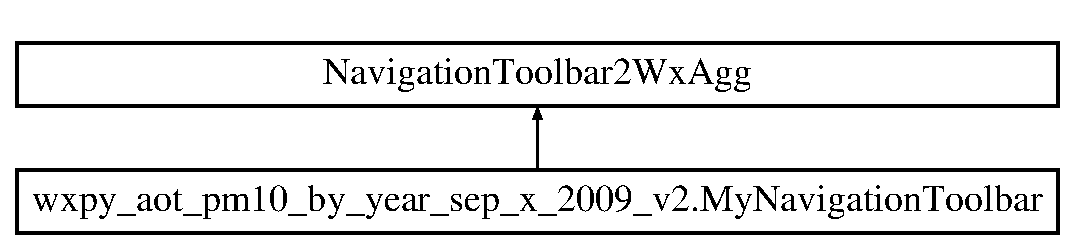
\includegraphics[height=2.000000cm]{classwxpy__aot__pm10__by__year__sep__x__2009__v2_1_1_my_navigation_toolbar}
\end{center}
\end{figure}
\subsection*{Fonctions membres publiques}
\begin{DoxyCompactItemize}
\item 
def \hyperlink{classwxpy__aot__pm10__by__year__sep__x__2009__v2_1_1_my_navigation_toolbar_a6549e51f96671d7c105978c88c282c7a}{\-\_\-\-\_\-init\-\_\-\-\_\-}
\item 
def \hyperlink{classwxpy__aot__pm10__by__year__sep__x__2009__v2_1_1_my_navigation_toolbar_acbcf931b3aae9895887d6eb46963ec06}{initmois}
\item 
def \hyperlink{classwxpy__aot__pm10__by__year__sep__x__2009__v2_1_1_my_navigation_toolbar_ad8bf8efd4d0099f5f191cb26f1a04187}{get\-\_\-jour\-\_\-en\-\_\-clair}
\item 
def \hyperlink{classwxpy__aot__pm10__by__year__sep__x__2009__v2_1_1_my_navigation_toolbar_a3a233a1ec5c603c87185eb275237ed2f}{get\-\_\-mois\-\_\-en\-\_\-clair}
\item 
def \hyperlink{classwxpy__aot__pm10__by__year__sep__x__2009__v2_1_1_my_navigation_toolbar_a36b25c375b8c1915b4ef80e1eafe79c9}{get\-\_\-string\-\_\-day}
\item 
def \hyperlink{classwxpy__aot__pm10__by__year__sep__x__2009__v2_1_1_my_navigation_toolbar_a0cbccfa3f773f80e6bc096e031efd29c}{getvg0n}
\item 
def \hyperlink{classwxpy__aot__pm10__by__year__sep__x__2009__v2_1_1_my_navigation_toolbar_aea4242e298f0515c2636c96d70f60f72}{getvg0\-\_\-month}
\item 
def \hyperlink{classwxpy__aot__pm10__by__year__sep__x__2009__v2_1_1_my_navigation_toolbar_a5d56e84bad8fe09fe1cefcdf96e52b7b}{getvg0\-\_\-2\-\_\-month}
\item 
def \hyperlink{classwxpy__aot__pm10__by__year__sep__x__2009__v2_1_1_my_navigation_toolbar_afc51cf51a72d3a48eaecd84d5c1577d0}{draw}
\item 
def \hyperlink{classwxpy__aot__pm10__by__year__sep__x__2009__v2_1_1_my_navigation_toolbar_ad203d350769a128fe37c96f4c0afaf68}{save}
\end{DoxyCompactItemize}
\subsection*{Attributs publics}
\begin{DoxyCompactItemize}
\item 
\hyperlink{classwxpy__aot__pm10__by__year__sep__x__2009__v2_1_1_my_navigation_toolbar_a04f32e366f8e5907fd79b32e7b6d99d4}{canvas}
\item 
\hyperlink{classwxpy__aot__pm10__by__year__sep__x__2009__v2_1_1_my_navigation_toolbar_a5c48272d04a0064308b59c18542015b4}{O\-N\-\_\-\-P\-R\-E\-V\-I\-O\-U\-S}
\item 
\hyperlink{classwxpy__aot__pm10__by__year__sep__x__2009__v2_1_1_my_navigation_toolbar_ad7f39ddcb9db500b4a9c8dd8ee3c44f9}{O\-N\-\_\-\-N\-E\-X\-T}
\item 
\hyperlink{classwxpy__aot__pm10__by__year__sep__x__2009__v2_1_1_my_navigation_toolbar_a29456a91d64ee106ffd9788103276f88}{O\-N\-\_\-\-L\-I\-S\-T\-E}
\item 
\hyperlink{classwxpy__aot__pm10__by__year__sep__x__2009__v2_1_1_my_navigation_toolbar_a667481ac1d94f5ab8abf6a0f37963746}{nmois}
\end{DoxyCompactItemize}
\subsection*{Attributs publics statiques}
\begin{DoxyCompactItemize}
\item 
tuple \hyperlink{classwxpy__aot__pm10__by__year__sep__x__2009__v2_1_1_my_navigation_toolbar_ac5120102131a18ea8112cdd8a9a833d0}{keys\-\_\-sort} = self.\-dirmois.\-keys()
\item 
tuple \hyperlink{classwxpy__aot__pm10__by__year__sep__x__2009__v2_1_1_my_navigation_toolbar_af99ad6e99a1567156f8b7990d5599467}{nweekday} = datefromday(2009,njour)
\item 
tuple \hyperlink{classwxpy__aot__pm10__by__year__sep__x__2009__v2_1_1_my_navigation_toolbar_a3598f315c51d9ed54f73cfa4766fa854}{dlg}
\item 
int \hyperlink{classwxpy__aot__pm10__by__year__sep__x__2009__v2_1_1_my_navigation_toolbar_ad9c4d0c94c929bd3e1b7ecf24dc89980}{indice} = 0
\item 
list \hyperlink{classwxpy__aot__pm10__by__year__sep__x__2009__v2_1_1_my_navigation_toolbar_a615093641e45188ca6eb62bd1fbccbed}{ax} = self.\-canvas.\-figure.\-axes\mbox{[}0\mbox{]}
\item 
int \hyperlink{classwxpy__aot__pm10__by__year__sep__x__2009__v2_1_1_my_navigation_toolbar_a9e969e3a61777d8ea92e7d6ffb4e1c06}{markersize} = 12
\end{DoxyCompactItemize}


\subsection{Description détaillée}
\begin{DoxyVerb}Extend the default wx toolbar with your own event handlers
\end{DoxyVerb}
 

\subsection{Documentation des constructeurs et destructeur}
\hypertarget{classwxpy__aot__pm10__by__year__sep__x__2009__v2_1_1_my_navigation_toolbar_a6549e51f96671d7c105978c88c282c7a}{\index{wxpy\-\_\-aot\-\_\-pm10\-\_\-by\-\_\-year\-\_\-sep\-\_\-x\-\_\-2009\-\_\-v2\-::\-My\-Navigation\-Toolbar@{wxpy\-\_\-aot\-\_\-pm10\-\_\-by\-\_\-year\-\_\-sep\-\_\-x\-\_\-2009\-\_\-v2\-::\-My\-Navigation\-Toolbar}!\-\_\-\-\_\-init\-\_\-\-\_\-@{\-\_\-\-\_\-init\-\_\-\-\_\-}}
\index{\-\_\-\-\_\-init\-\_\-\-\_\-@{\-\_\-\-\_\-init\-\_\-\-\_\-}!wxpy_aot_pm10_by_year_sep_x_2009_v2::MyNavigationToolbar@{wxpy\-\_\-aot\-\_\-pm10\-\_\-by\-\_\-year\-\_\-sep\-\_\-x\-\_\-2009\-\_\-v2\-::\-My\-Navigation\-Toolbar}}
\subsubsection[{\-\_\-\-\_\-init\-\_\-\-\_\-}]{\setlength{\rightskip}{0pt plus 5cm}def wxpy\-\_\-aot\-\_\-pm10\-\_\-by\-\_\-year\-\_\-sep\-\_\-x\-\_\-2009\-\_\-v2.\-My\-Navigation\-Toolbar.\-\_\-\-\_\-init\-\_\-\-\_\- (
\begin{DoxyParamCaption}
\item[{}]{self, }
\item[{}]{canvas, }
\item[{}]{cankill}
\end{DoxyParamCaption}
)}}\label{classwxpy__aot__pm10__by__year__sep__x__2009__v2_1_1_my_navigation_toolbar_a6549e51f96671d7c105978c88c282c7a}


\subsection{Documentation des fonctions membres}
\hypertarget{classwxpy__aot__pm10__by__year__sep__x__2009__v2_1_1_my_navigation_toolbar_afc51cf51a72d3a48eaecd84d5c1577d0}{\index{wxpy\-\_\-aot\-\_\-pm10\-\_\-by\-\_\-year\-\_\-sep\-\_\-x\-\_\-2009\-\_\-v2\-::\-My\-Navigation\-Toolbar@{wxpy\-\_\-aot\-\_\-pm10\-\_\-by\-\_\-year\-\_\-sep\-\_\-x\-\_\-2009\-\_\-v2\-::\-My\-Navigation\-Toolbar}!draw@{draw}}
\index{draw@{draw}!wxpy_aot_pm10_by_year_sep_x_2009_v2::MyNavigationToolbar@{wxpy\-\_\-aot\-\_\-pm10\-\_\-by\-\_\-year\-\_\-sep\-\_\-x\-\_\-2009\-\_\-v2\-::\-My\-Navigation\-Toolbar}}
\subsubsection[{draw}]{\setlength{\rightskip}{0pt plus 5cm}def wxpy\-\_\-aot\-\_\-pm10\-\_\-by\-\_\-year\-\_\-sep\-\_\-x\-\_\-2009\-\_\-v2.\-My\-Navigation\-Toolbar.\-draw (
\begin{DoxyParamCaption}
\item[{}]{self, }
\item[{}]{args}
\end{DoxyParamCaption}
)}}\label{classwxpy__aot__pm10__by__year__sep__x__2009__v2_1_1_my_navigation_toolbar_afc51cf51a72d3a48eaecd84d5c1577d0}
\begin{DoxyVerb}Tracer les courbes en fonction de la date choisie \end{DoxyVerb}
 \hypertarget{classwxpy__aot__pm10__by__year__sep__x__2009__v2_1_1_my_navigation_toolbar_ad8bf8efd4d0099f5f191cb26f1a04187}{\index{wxpy\-\_\-aot\-\_\-pm10\-\_\-by\-\_\-year\-\_\-sep\-\_\-x\-\_\-2009\-\_\-v2\-::\-My\-Navigation\-Toolbar@{wxpy\-\_\-aot\-\_\-pm10\-\_\-by\-\_\-year\-\_\-sep\-\_\-x\-\_\-2009\-\_\-v2\-::\-My\-Navigation\-Toolbar}!get\-\_\-jour\-\_\-en\-\_\-clair@{get\-\_\-jour\-\_\-en\-\_\-clair}}
\index{get\-\_\-jour\-\_\-en\-\_\-clair@{get\-\_\-jour\-\_\-en\-\_\-clair}!wxpy_aot_pm10_by_year_sep_x_2009_v2::MyNavigationToolbar@{wxpy\-\_\-aot\-\_\-pm10\-\_\-by\-\_\-year\-\_\-sep\-\_\-x\-\_\-2009\-\_\-v2\-::\-My\-Navigation\-Toolbar}}
\subsubsection[{get\-\_\-jour\-\_\-en\-\_\-clair}]{\setlength{\rightskip}{0pt plus 5cm}def wxpy\-\_\-aot\-\_\-pm10\-\_\-by\-\_\-year\-\_\-sep\-\_\-x\-\_\-2009\-\_\-v2.\-My\-Navigation\-Toolbar.\-get\-\_\-jour\-\_\-en\-\_\-clair (
\begin{DoxyParamCaption}
\item[{}]{self, }
\item[{}]{njour}
\end{DoxyParamCaption}
)}}\label{classwxpy__aot__pm10__by__year__sep__x__2009__v2_1_1_my_navigation_toolbar_ad8bf8efd4d0099f5f191cb26f1a04187}
\hypertarget{classwxpy__aot__pm10__by__year__sep__x__2009__v2_1_1_my_navigation_toolbar_a3a233a1ec5c603c87185eb275237ed2f}{\index{wxpy\-\_\-aot\-\_\-pm10\-\_\-by\-\_\-year\-\_\-sep\-\_\-x\-\_\-2009\-\_\-v2\-::\-My\-Navigation\-Toolbar@{wxpy\-\_\-aot\-\_\-pm10\-\_\-by\-\_\-year\-\_\-sep\-\_\-x\-\_\-2009\-\_\-v2\-::\-My\-Navigation\-Toolbar}!get\-\_\-mois\-\_\-en\-\_\-clair@{get\-\_\-mois\-\_\-en\-\_\-clair}}
\index{get\-\_\-mois\-\_\-en\-\_\-clair@{get\-\_\-mois\-\_\-en\-\_\-clair}!wxpy_aot_pm10_by_year_sep_x_2009_v2::MyNavigationToolbar@{wxpy\-\_\-aot\-\_\-pm10\-\_\-by\-\_\-year\-\_\-sep\-\_\-x\-\_\-2009\-\_\-v2\-::\-My\-Navigation\-Toolbar}}
\subsubsection[{get\-\_\-mois\-\_\-en\-\_\-clair}]{\setlength{\rightskip}{0pt plus 5cm}def wxpy\-\_\-aot\-\_\-pm10\-\_\-by\-\_\-year\-\_\-sep\-\_\-x\-\_\-2009\-\_\-v2.\-My\-Navigation\-Toolbar.\-get\-\_\-mois\-\_\-en\-\_\-clair (
\begin{DoxyParamCaption}
\item[{}]{self, }
\item[{}]{nmois}
\end{DoxyParamCaption}
)}}\label{classwxpy__aot__pm10__by__year__sep__x__2009__v2_1_1_my_navigation_toolbar_a3a233a1ec5c603c87185eb275237ed2f}
\begin{DoxyVerb}Renvoyer le mois en texte � partir du n�\end{DoxyVerb}
 \hypertarget{classwxpy__aot__pm10__by__year__sep__x__2009__v2_1_1_my_navigation_toolbar_a36b25c375b8c1915b4ef80e1eafe79c9}{\index{wxpy\-\_\-aot\-\_\-pm10\-\_\-by\-\_\-year\-\_\-sep\-\_\-x\-\_\-2009\-\_\-v2\-::\-My\-Navigation\-Toolbar@{wxpy\-\_\-aot\-\_\-pm10\-\_\-by\-\_\-year\-\_\-sep\-\_\-x\-\_\-2009\-\_\-v2\-::\-My\-Navigation\-Toolbar}!get\-\_\-string\-\_\-day@{get\-\_\-string\-\_\-day}}
\index{get\-\_\-string\-\_\-day@{get\-\_\-string\-\_\-day}!wxpy_aot_pm10_by_year_sep_x_2009_v2::MyNavigationToolbar@{wxpy\-\_\-aot\-\_\-pm10\-\_\-by\-\_\-year\-\_\-sep\-\_\-x\-\_\-2009\-\_\-v2\-::\-My\-Navigation\-Toolbar}}
\subsubsection[{get\-\_\-string\-\_\-day}]{\setlength{\rightskip}{0pt plus 5cm}def wxpy\-\_\-aot\-\_\-pm10\-\_\-by\-\_\-year\-\_\-sep\-\_\-x\-\_\-2009\-\_\-v2.\-My\-Navigation\-Toolbar.\-get\-\_\-string\-\_\-day (
\begin{DoxyParamCaption}
\item[{}]{self, }
\item[{}]{njour}
\end{DoxyParamCaption}
)}}\label{classwxpy__aot__pm10__by__year__sep__x__2009__v2_1_1_my_navigation_toolbar_a36b25c375b8c1915b4ef80e1eafe79c9}
\hypertarget{classwxpy__aot__pm10__by__year__sep__x__2009__v2_1_1_my_navigation_toolbar_a5d56e84bad8fe09fe1cefcdf96e52b7b}{\index{wxpy\-\_\-aot\-\_\-pm10\-\_\-by\-\_\-year\-\_\-sep\-\_\-x\-\_\-2009\-\_\-v2\-::\-My\-Navigation\-Toolbar@{wxpy\-\_\-aot\-\_\-pm10\-\_\-by\-\_\-year\-\_\-sep\-\_\-x\-\_\-2009\-\_\-v2\-::\-My\-Navigation\-Toolbar}!getvg0\-\_\-2\-\_\-month@{getvg0\-\_\-2\-\_\-month}}
\index{getvg0\-\_\-2\-\_\-month@{getvg0\-\_\-2\-\_\-month}!wxpy_aot_pm10_by_year_sep_x_2009_v2::MyNavigationToolbar@{wxpy\-\_\-aot\-\_\-pm10\-\_\-by\-\_\-year\-\_\-sep\-\_\-x\-\_\-2009\-\_\-v2\-::\-My\-Navigation\-Toolbar}}
\subsubsection[{getvg0\-\_\-2\-\_\-month}]{\setlength{\rightskip}{0pt plus 5cm}def wxpy\-\_\-aot\-\_\-pm10\-\_\-by\-\_\-year\-\_\-sep\-\_\-x\-\_\-2009\-\_\-v2.\-My\-Navigation\-Toolbar.\-getvg0\-\_\-2\-\_\-month (
\begin{DoxyParamCaption}
\item[{}]{self, }
\item[{}]{nmonth}
\end{DoxyParamCaption}
)}}\label{classwxpy__aot__pm10__by__year__sep__x__2009__v2_1_1_my_navigation_toolbar_a5d56e84bad8fe09fe1cefcdf96e52b7b}
\begin{DoxyVerb}Select a month of data \end{DoxyVerb}
 \hypertarget{classwxpy__aot__pm10__by__year__sep__x__2009__v2_1_1_my_navigation_toolbar_aea4242e298f0515c2636c96d70f60f72}{\index{wxpy\-\_\-aot\-\_\-pm10\-\_\-by\-\_\-year\-\_\-sep\-\_\-x\-\_\-2009\-\_\-v2\-::\-My\-Navigation\-Toolbar@{wxpy\-\_\-aot\-\_\-pm10\-\_\-by\-\_\-year\-\_\-sep\-\_\-x\-\_\-2009\-\_\-v2\-::\-My\-Navigation\-Toolbar}!getvg0\-\_\-month@{getvg0\-\_\-month}}
\index{getvg0\-\_\-month@{getvg0\-\_\-month}!wxpy_aot_pm10_by_year_sep_x_2009_v2::MyNavigationToolbar@{wxpy\-\_\-aot\-\_\-pm10\-\_\-by\-\_\-year\-\_\-sep\-\_\-x\-\_\-2009\-\_\-v2\-::\-My\-Navigation\-Toolbar}}
\subsubsection[{getvg0\-\_\-month}]{\setlength{\rightskip}{0pt plus 5cm}def wxpy\-\_\-aot\-\_\-pm10\-\_\-by\-\_\-year\-\_\-sep\-\_\-x\-\_\-2009\-\_\-v2.\-My\-Navigation\-Toolbar.\-getvg0\-\_\-month (
\begin{DoxyParamCaption}
\item[{}]{self, }
\item[{}]{nmonth}
\end{DoxyParamCaption}
)}}\label{classwxpy__aot__pm10__by__year__sep__x__2009__v2_1_1_my_navigation_toolbar_aea4242e298f0515c2636c96d70f60f72}
\begin{DoxyVerb}Select a month of data \end{DoxyVerb}
 \hypertarget{classwxpy__aot__pm10__by__year__sep__x__2009__v2_1_1_my_navigation_toolbar_a0cbccfa3f773f80e6bc096e031efd29c}{\index{wxpy\-\_\-aot\-\_\-pm10\-\_\-by\-\_\-year\-\_\-sep\-\_\-x\-\_\-2009\-\_\-v2\-::\-My\-Navigation\-Toolbar@{wxpy\-\_\-aot\-\_\-pm10\-\_\-by\-\_\-year\-\_\-sep\-\_\-x\-\_\-2009\-\_\-v2\-::\-My\-Navigation\-Toolbar}!getvg0n@{getvg0n}}
\index{getvg0n@{getvg0n}!wxpy_aot_pm10_by_year_sep_x_2009_v2::MyNavigationToolbar@{wxpy\-\_\-aot\-\_\-pm10\-\_\-by\-\_\-year\-\_\-sep\-\_\-x\-\_\-2009\-\_\-v2\-::\-My\-Navigation\-Toolbar}}
\subsubsection[{getvg0n}]{\setlength{\rightskip}{0pt plus 5cm}def wxpy\-\_\-aot\-\_\-pm10\-\_\-by\-\_\-year\-\_\-sep\-\_\-x\-\_\-2009\-\_\-v2.\-My\-Navigation\-Toolbar.\-getvg0n (
\begin{DoxyParamCaption}
\item[{}]{self, }
\item[{}]{nday}
\end{DoxyParamCaption}
)}}\label{classwxpy__aot__pm10__by__year__sep__x__2009__v2_1_1_my_navigation_toolbar_a0cbccfa3f773f80e6bc096e031efd29c}
\begin{DoxyVerb}Select a day of data \end{DoxyVerb}
 \hypertarget{classwxpy__aot__pm10__by__year__sep__x__2009__v2_1_1_my_navigation_toolbar_acbcf931b3aae9895887d6eb46963ec06}{\index{wxpy\-\_\-aot\-\_\-pm10\-\_\-by\-\_\-year\-\_\-sep\-\_\-x\-\_\-2009\-\_\-v2\-::\-My\-Navigation\-Toolbar@{wxpy\-\_\-aot\-\_\-pm10\-\_\-by\-\_\-year\-\_\-sep\-\_\-x\-\_\-2009\-\_\-v2\-::\-My\-Navigation\-Toolbar}!initmois@{initmois}}
\index{initmois@{initmois}!wxpy_aot_pm10_by_year_sep_x_2009_v2::MyNavigationToolbar@{wxpy\-\_\-aot\-\_\-pm10\-\_\-by\-\_\-year\-\_\-sep\-\_\-x\-\_\-2009\-\_\-v2\-::\-My\-Navigation\-Toolbar}}
\subsubsection[{initmois}]{\setlength{\rightskip}{0pt plus 5cm}def wxpy\-\_\-aot\-\_\-pm10\-\_\-by\-\_\-year\-\_\-sep\-\_\-x\-\_\-2009\-\_\-v2.\-My\-Navigation\-Toolbar.\-initmois (
\begin{DoxyParamCaption}
\item[{}]{self}
\end{DoxyParamCaption}
)}}\label{classwxpy__aot__pm10__by__year__sep__x__2009__v2_1_1_my_navigation_toolbar_acbcf931b3aae9895887d6eb46963ec06}
\begin{DoxyVerb}Init months  \end{DoxyVerb}
 \hypertarget{classwxpy__aot__pm10__by__year__sep__x__2009__v2_1_1_my_navigation_toolbar_ad203d350769a128fe37c96f4c0afaf68}{\index{wxpy\-\_\-aot\-\_\-pm10\-\_\-by\-\_\-year\-\_\-sep\-\_\-x\-\_\-2009\-\_\-v2\-::\-My\-Navigation\-Toolbar@{wxpy\-\_\-aot\-\_\-pm10\-\_\-by\-\_\-year\-\_\-sep\-\_\-x\-\_\-2009\-\_\-v2\-::\-My\-Navigation\-Toolbar}!save@{save}}
\index{save@{save}!wxpy_aot_pm10_by_year_sep_x_2009_v2::MyNavigationToolbar@{wxpy\-\_\-aot\-\_\-pm10\-\_\-by\-\_\-year\-\_\-sep\-\_\-x\-\_\-2009\-\_\-v2\-::\-My\-Navigation\-Toolbar}}
\subsubsection[{save}]{\setlength{\rightskip}{0pt plus 5cm}def wxpy\-\_\-aot\-\_\-pm10\-\_\-by\-\_\-year\-\_\-sep\-\_\-x\-\_\-2009\-\_\-v2.\-My\-Navigation\-Toolbar.\-save (
\begin{DoxyParamCaption}
\item[{}]{self, }
\item[{}]{evt}
\end{DoxyParamCaption}
)}}\label{classwxpy__aot__pm10__by__year__sep__x__2009__v2_1_1_my_navigation_toolbar_ad203d350769a128fe37c96f4c0afaf68}
\begin{DoxyVerb}Save figure without prompting for a location \end{DoxyVerb}
 

\subsection{Documentation des données membres}
\hypertarget{classwxpy__aot__pm10__by__year__sep__x__2009__v2_1_1_my_navigation_toolbar_a615093641e45188ca6eb62bd1fbccbed}{\index{wxpy\-\_\-aot\-\_\-pm10\-\_\-by\-\_\-year\-\_\-sep\-\_\-x\-\_\-2009\-\_\-v2\-::\-My\-Navigation\-Toolbar@{wxpy\-\_\-aot\-\_\-pm10\-\_\-by\-\_\-year\-\_\-sep\-\_\-x\-\_\-2009\-\_\-v2\-::\-My\-Navigation\-Toolbar}!ax@{ax}}
\index{ax@{ax}!wxpy_aot_pm10_by_year_sep_x_2009_v2::MyNavigationToolbar@{wxpy\-\_\-aot\-\_\-pm10\-\_\-by\-\_\-year\-\_\-sep\-\_\-x\-\_\-2009\-\_\-v2\-::\-My\-Navigation\-Toolbar}}
\subsubsection[{ax}]{\setlength{\rightskip}{0pt plus 5cm}list wxpy\-\_\-aot\-\_\-pm10\-\_\-by\-\_\-year\-\_\-sep\-\_\-x\-\_\-2009\-\_\-v2.\-My\-Navigation\-Toolbar.\-ax = self.\-canvas.\-figure.\-axes\mbox{[}0\mbox{]}\hspace{0.3cm}{\ttfamily [static]}}}\label{classwxpy__aot__pm10__by__year__sep__x__2009__v2_1_1_my_navigation_toolbar_a615093641e45188ca6eb62bd1fbccbed}
\hypertarget{classwxpy__aot__pm10__by__year__sep__x__2009__v2_1_1_my_navigation_toolbar_a04f32e366f8e5907fd79b32e7b6d99d4}{\index{wxpy\-\_\-aot\-\_\-pm10\-\_\-by\-\_\-year\-\_\-sep\-\_\-x\-\_\-2009\-\_\-v2\-::\-My\-Navigation\-Toolbar@{wxpy\-\_\-aot\-\_\-pm10\-\_\-by\-\_\-year\-\_\-sep\-\_\-x\-\_\-2009\-\_\-v2\-::\-My\-Navigation\-Toolbar}!canvas@{canvas}}
\index{canvas@{canvas}!wxpy_aot_pm10_by_year_sep_x_2009_v2::MyNavigationToolbar@{wxpy\-\_\-aot\-\_\-pm10\-\_\-by\-\_\-year\-\_\-sep\-\_\-x\-\_\-2009\-\_\-v2\-::\-My\-Navigation\-Toolbar}}
\subsubsection[{canvas}]{\setlength{\rightskip}{0pt plus 5cm}wxpy\-\_\-aot\-\_\-pm10\-\_\-by\-\_\-year\-\_\-sep\-\_\-x\-\_\-2009\-\_\-v2.\-My\-Navigation\-Toolbar.\-canvas}}\label{classwxpy__aot__pm10__by__year__sep__x__2009__v2_1_1_my_navigation_toolbar_a04f32e366f8e5907fd79b32e7b6d99d4}
\hypertarget{classwxpy__aot__pm10__by__year__sep__x__2009__v2_1_1_my_navigation_toolbar_a3598f315c51d9ed54f73cfa4766fa854}{\index{wxpy\-\_\-aot\-\_\-pm10\-\_\-by\-\_\-year\-\_\-sep\-\_\-x\-\_\-2009\-\_\-v2\-::\-My\-Navigation\-Toolbar@{wxpy\-\_\-aot\-\_\-pm10\-\_\-by\-\_\-year\-\_\-sep\-\_\-x\-\_\-2009\-\_\-v2\-::\-My\-Navigation\-Toolbar}!dlg@{dlg}}
\index{dlg@{dlg}!wxpy_aot_pm10_by_year_sep_x_2009_v2::MyNavigationToolbar@{wxpy\-\_\-aot\-\_\-pm10\-\_\-by\-\_\-year\-\_\-sep\-\_\-x\-\_\-2009\-\_\-v2\-::\-My\-Navigation\-Toolbar}}
\subsubsection[{dlg}]{\setlength{\rightskip}{0pt plus 5cm}tuple wxpy\-\_\-aot\-\_\-pm10\-\_\-by\-\_\-year\-\_\-sep\-\_\-x\-\_\-2009\-\_\-v2.\-My\-Navigation\-Toolbar.\-dlg\hspace{0.3cm}{\ttfamily [static]}}}\label{classwxpy__aot__pm10__by__year__sep__x__2009__v2_1_1_my_navigation_toolbar_a3598f315c51d9ed54f73cfa4766fa854}
{\bfseries Valeur initiale \-:}
\begin{DoxyCode}
1 = wx.SingleChoiceDialog(
2                 self, \textcolor{stringliteral}{'Choisir un mois'}, \textcolor{stringliteral}{'Veuille choisir un mois'},
3                 [str(nmois) \textcolor{keywordflow}{for} nmois \textcolor{keywordflow}{in} list(self.datamois)],
4                 wx.CHOICEDLG\_STYLE
5                 )
\end{DoxyCode}
\hypertarget{classwxpy__aot__pm10__by__year__sep__x__2009__v2_1_1_my_navigation_toolbar_ad9c4d0c94c929bd3e1b7ecf24dc89980}{\index{wxpy\-\_\-aot\-\_\-pm10\-\_\-by\-\_\-year\-\_\-sep\-\_\-x\-\_\-2009\-\_\-v2\-::\-My\-Navigation\-Toolbar@{wxpy\-\_\-aot\-\_\-pm10\-\_\-by\-\_\-year\-\_\-sep\-\_\-x\-\_\-2009\-\_\-v2\-::\-My\-Navigation\-Toolbar}!indice@{indice}}
\index{indice@{indice}!wxpy_aot_pm10_by_year_sep_x_2009_v2::MyNavigationToolbar@{wxpy\-\_\-aot\-\_\-pm10\-\_\-by\-\_\-year\-\_\-sep\-\_\-x\-\_\-2009\-\_\-v2\-::\-My\-Navigation\-Toolbar}}
\subsubsection[{indice}]{\setlength{\rightskip}{0pt plus 5cm}int wxpy\-\_\-aot\-\_\-pm10\-\_\-by\-\_\-year\-\_\-sep\-\_\-x\-\_\-2009\-\_\-v2.\-My\-Navigation\-Toolbar.\-indice = 0\hspace{0.3cm}{\ttfamily [static]}}}\label{classwxpy__aot__pm10__by__year__sep__x__2009__v2_1_1_my_navigation_toolbar_ad9c4d0c94c929bd3e1b7ecf24dc89980}
\hypertarget{classwxpy__aot__pm10__by__year__sep__x__2009__v2_1_1_my_navigation_toolbar_ac5120102131a18ea8112cdd8a9a833d0}{\index{wxpy\-\_\-aot\-\_\-pm10\-\_\-by\-\_\-year\-\_\-sep\-\_\-x\-\_\-2009\-\_\-v2\-::\-My\-Navigation\-Toolbar@{wxpy\-\_\-aot\-\_\-pm10\-\_\-by\-\_\-year\-\_\-sep\-\_\-x\-\_\-2009\-\_\-v2\-::\-My\-Navigation\-Toolbar}!keys\-\_\-sort@{keys\-\_\-sort}}
\index{keys\-\_\-sort@{keys\-\_\-sort}!wxpy_aot_pm10_by_year_sep_x_2009_v2::MyNavigationToolbar@{wxpy\-\_\-aot\-\_\-pm10\-\_\-by\-\_\-year\-\_\-sep\-\_\-x\-\_\-2009\-\_\-v2\-::\-My\-Navigation\-Toolbar}}
\subsubsection[{keys\-\_\-sort}]{\setlength{\rightskip}{0pt plus 5cm}tuple wxpy\-\_\-aot\-\_\-pm10\-\_\-by\-\_\-year\-\_\-sep\-\_\-x\-\_\-2009\-\_\-v2.\-My\-Navigation\-Toolbar.\-keys\-\_\-sort = self.\-dirmois.\-keys()\hspace{0.3cm}{\ttfamily [static]}}}\label{classwxpy__aot__pm10__by__year__sep__x__2009__v2_1_1_my_navigation_toolbar_ac5120102131a18ea8112cdd8a9a833d0}
\hypertarget{classwxpy__aot__pm10__by__year__sep__x__2009__v2_1_1_my_navigation_toolbar_a9e969e3a61777d8ea92e7d6ffb4e1c06}{\index{wxpy\-\_\-aot\-\_\-pm10\-\_\-by\-\_\-year\-\_\-sep\-\_\-x\-\_\-2009\-\_\-v2\-::\-My\-Navigation\-Toolbar@{wxpy\-\_\-aot\-\_\-pm10\-\_\-by\-\_\-year\-\_\-sep\-\_\-x\-\_\-2009\-\_\-v2\-::\-My\-Navigation\-Toolbar}!markersize@{markersize}}
\index{markersize@{markersize}!wxpy_aot_pm10_by_year_sep_x_2009_v2::MyNavigationToolbar@{wxpy\-\_\-aot\-\_\-pm10\-\_\-by\-\_\-year\-\_\-sep\-\_\-x\-\_\-2009\-\_\-v2\-::\-My\-Navigation\-Toolbar}}
\subsubsection[{markersize}]{\setlength{\rightskip}{0pt plus 5cm}int wxpy\-\_\-aot\-\_\-pm10\-\_\-by\-\_\-year\-\_\-sep\-\_\-x\-\_\-2009\-\_\-v2.\-My\-Navigation\-Toolbar.\-markersize = 12\hspace{0.3cm}{\ttfamily [static]}}}\label{classwxpy__aot__pm10__by__year__sep__x__2009__v2_1_1_my_navigation_toolbar_a9e969e3a61777d8ea92e7d6ffb4e1c06}
\hypertarget{classwxpy__aot__pm10__by__year__sep__x__2009__v2_1_1_my_navigation_toolbar_a667481ac1d94f5ab8abf6a0f37963746}{\index{wxpy\-\_\-aot\-\_\-pm10\-\_\-by\-\_\-year\-\_\-sep\-\_\-x\-\_\-2009\-\_\-v2\-::\-My\-Navigation\-Toolbar@{wxpy\-\_\-aot\-\_\-pm10\-\_\-by\-\_\-year\-\_\-sep\-\_\-x\-\_\-2009\-\_\-v2\-::\-My\-Navigation\-Toolbar}!nmois@{nmois}}
\index{nmois@{nmois}!wxpy_aot_pm10_by_year_sep_x_2009_v2::MyNavigationToolbar@{wxpy\-\_\-aot\-\_\-pm10\-\_\-by\-\_\-year\-\_\-sep\-\_\-x\-\_\-2009\-\_\-v2\-::\-My\-Navigation\-Toolbar}}
\subsubsection[{nmois}]{\setlength{\rightskip}{0pt plus 5cm}wxpy\-\_\-aot\-\_\-pm10\-\_\-by\-\_\-year\-\_\-sep\-\_\-x\-\_\-2009\-\_\-v2.\-My\-Navigation\-Toolbar.\-nmois}}\label{classwxpy__aot__pm10__by__year__sep__x__2009__v2_1_1_my_navigation_toolbar_a667481ac1d94f5ab8abf6a0f37963746}
\hypertarget{classwxpy__aot__pm10__by__year__sep__x__2009__v2_1_1_my_navigation_toolbar_af99ad6e99a1567156f8b7990d5599467}{\index{wxpy\-\_\-aot\-\_\-pm10\-\_\-by\-\_\-year\-\_\-sep\-\_\-x\-\_\-2009\-\_\-v2\-::\-My\-Navigation\-Toolbar@{wxpy\-\_\-aot\-\_\-pm10\-\_\-by\-\_\-year\-\_\-sep\-\_\-x\-\_\-2009\-\_\-v2\-::\-My\-Navigation\-Toolbar}!nweekday@{nweekday}}
\index{nweekday@{nweekday}!wxpy_aot_pm10_by_year_sep_x_2009_v2::MyNavigationToolbar@{wxpy\-\_\-aot\-\_\-pm10\-\_\-by\-\_\-year\-\_\-sep\-\_\-x\-\_\-2009\-\_\-v2\-::\-My\-Navigation\-Toolbar}}
\subsubsection[{nweekday}]{\setlength{\rightskip}{0pt plus 5cm}tuple wxpy\-\_\-aot\-\_\-pm10\-\_\-by\-\_\-year\-\_\-sep\-\_\-x\-\_\-2009\-\_\-v2.\-My\-Navigation\-Toolbar.\-nweekday = datefromday(2009,njour)\hspace{0.3cm}{\ttfamily [static]}}}\label{classwxpy__aot__pm10__by__year__sep__x__2009__v2_1_1_my_navigation_toolbar_af99ad6e99a1567156f8b7990d5599467}
\hypertarget{classwxpy__aot__pm10__by__year__sep__x__2009__v2_1_1_my_navigation_toolbar_a29456a91d64ee106ffd9788103276f88}{\index{wxpy\-\_\-aot\-\_\-pm10\-\_\-by\-\_\-year\-\_\-sep\-\_\-x\-\_\-2009\-\_\-v2\-::\-My\-Navigation\-Toolbar@{wxpy\-\_\-aot\-\_\-pm10\-\_\-by\-\_\-year\-\_\-sep\-\_\-x\-\_\-2009\-\_\-v2\-::\-My\-Navigation\-Toolbar}!O\-N\-\_\-\-L\-I\-S\-T\-E@{O\-N\-\_\-\-L\-I\-S\-T\-E}}
\index{O\-N\-\_\-\-L\-I\-S\-T\-E@{O\-N\-\_\-\-L\-I\-S\-T\-E}!wxpy_aot_pm10_by_year_sep_x_2009_v2::MyNavigationToolbar@{wxpy\-\_\-aot\-\_\-pm10\-\_\-by\-\_\-year\-\_\-sep\-\_\-x\-\_\-2009\-\_\-v2\-::\-My\-Navigation\-Toolbar}}
\subsubsection[{O\-N\-\_\-\-L\-I\-S\-T\-E}]{\setlength{\rightskip}{0pt plus 5cm}wxpy\-\_\-aot\-\_\-pm10\-\_\-by\-\_\-year\-\_\-sep\-\_\-x\-\_\-2009\-\_\-v2.\-My\-Navigation\-Toolbar.\-O\-N\-\_\-\-L\-I\-S\-T\-E}}\label{classwxpy__aot__pm10__by__year__sep__x__2009__v2_1_1_my_navigation_toolbar_a29456a91d64ee106ffd9788103276f88}
\hypertarget{classwxpy__aot__pm10__by__year__sep__x__2009__v2_1_1_my_navigation_toolbar_ad7f39ddcb9db500b4a9c8dd8ee3c44f9}{\index{wxpy\-\_\-aot\-\_\-pm10\-\_\-by\-\_\-year\-\_\-sep\-\_\-x\-\_\-2009\-\_\-v2\-::\-My\-Navigation\-Toolbar@{wxpy\-\_\-aot\-\_\-pm10\-\_\-by\-\_\-year\-\_\-sep\-\_\-x\-\_\-2009\-\_\-v2\-::\-My\-Navigation\-Toolbar}!O\-N\-\_\-\-N\-E\-X\-T@{O\-N\-\_\-\-N\-E\-X\-T}}
\index{O\-N\-\_\-\-N\-E\-X\-T@{O\-N\-\_\-\-N\-E\-X\-T}!wxpy_aot_pm10_by_year_sep_x_2009_v2::MyNavigationToolbar@{wxpy\-\_\-aot\-\_\-pm10\-\_\-by\-\_\-year\-\_\-sep\-\_\-x\-\_\-2009\-\_\-v2\-::\-My\-Navigation\-Toolbar}}
\subsubsection[{O\-N\-\_\-\-N\-E\-X\-T}]{\setlength{\rightskip}{0pt plus 5cm}wxpy\-\_\-aot\-\_\-pm10\-\_\-by\-\_\-year\-\_\-sep\-\_\-x\-\_\-2009\-\_\-v2.\-My\-Navigation\-Toolbar.\-O\-N\-\_\-\-N\-E\-X\-T}}\label{classwxpy__aot__pm10__by__year__sep__x__2009__v2_1_1_my_navigation_toolbar_ad7f39ddcb9db500b4a9c8dd8ee3c44f9}
\hypertarget{classwxpy__aot__pm10__by__year__sep__x__2009__v2_1_1_my_navigation_toolbar_a5c48272d04a0064308b59c18542015b4}{\index{wxpy\-\_\-aot\-\_\-pm10\-\_\-by\-\_\-year\-\_\-sep\-\_\-x\-\_\-2009\-\_\-v2\-::\-My\-Navigation\-Toolbar@{wxpy\-\_\-aot\-\_\-pm10\-\_\-by\-\_\-year\-\_\-sep\-\_\-x\-\_\-2009\-\_\-v2\-::\-My\-Navigation\-Toolbar}!O\-N\-\_\-\-P\-R\-E\-V\-I\-O\-U\-S@{O\-N\-\_\-\-P\-R\-E\-V\-I\-O\-U\-S}}
\index{O\-N\-\_\-\-P\-R\-E\-V\-I\-O\-U\-S@{O\-N\-\_\-\-P\-R\-E\-V\-I\-O\-U\-S}!wxpy_aot_pm10_by_year_sep_x_2009_v2::MyNavigationToolbar@{wxpy\-\_\-aot\-\_\-pm10\-\_\-by\-\_\-year\-\_\-sep\-\_\-x\-\_\-2009\-\_\-v2\-::\-My\-Navigation\-Toolbar}}
\subsubsection[{O\-N\-\_\-\-P\-R\-E\-V\-I\-O\-U\-S}]{\setlength{\rightskip}{0pt plus 5cm}wxpy\-\_\-aot\-\_\-pm10\-\_\-by\-\_\-year\-\_\-sep\-\_\-x\-\_\-2009\-\_\-v2.\-My\-Navigation\-Toolbar.\-O\-N\-\_\-\-P\-R\-E\-V\-I\-O\-U\-S}}\label{classwxpy__aot__pm10__by__year__sep__x__2009__v2_1_1_my_navigation_toolbar_a5c48272d04a0064308b59c18542015b4}


La documentation de cette classe a été générée à partir du fichier suivant \-:\begin{DoxyCompactItemize}
\item 
\hyperlink{wxpy__aot__pm10__by__year__sep__x__2009__v2_8py}{wxpy\-\_\-aot\-\_\-pm10\-\_\-by\-\_\-year\-\_\-sep\-\_\-x\-\_\-2009\-\_\-v2.\-py}\end{DoxyCompactItemize}

\hypertarget{classwxpy__aot__pm10__by__years_1_1_my_navigation_toolbar}{\section{Référence de la classe wxpy\-\_\-aot\-\_\-pm10\-\_\-by\-\_\-years.\-My\-Navigation\-Toolbar}
\label{classwxpy__aot__pm10__by__years_1_1_my_navigation_toolbar}\index{wxpy\-\_\-aot\-\_\-pm10\-\_\-by\-\_\-years.\-My\-Navigation\-Toolbar@{wxpy\-\_\-aot\-\_\-pm10\-\_\-by\-\_\-years.\-My\-Navigation\-Toolbar}}
}
Graphe d'héritage de wxpy\-\_\-aot\-\_\-pm10\-\_\-by\-\_\-years.\-My\-Navigation\-Toolbar\-:\begin{figure}[H]
\begin{center}
\leavevmode
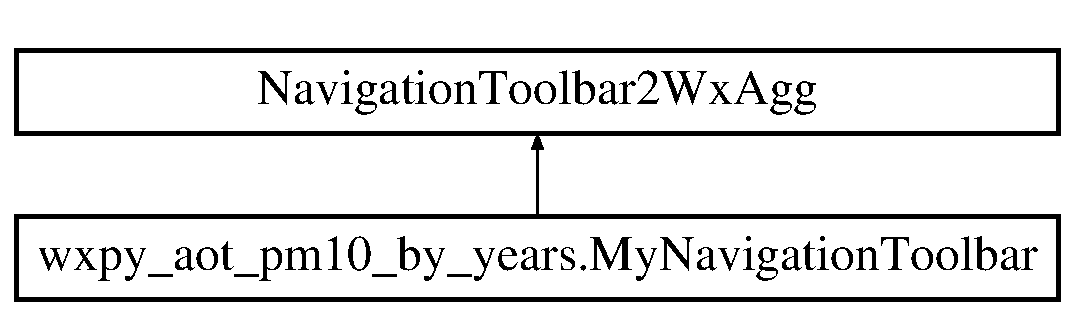
\includegraphics[height=2.000000cm]{classwxpy__aot__pm10__by__years_1_1_my_navigation_toolbar}
\end{center}
\end{figure}
\subsection*{Fonctions membres publiques}
\begin{DoxyCompactItemize}
\item 
def \hyperlink{classwxpy__aot__pm10__by__years_1_1_my_navigation_toolbar_ab4ef95699404501f88423e2d2cc93c48}{\-\_\-\-\_\-init\-\_\-\-\_\-}
\item 
def \hyperlink{classwxpy__aot__pm10__by__years_1_1_my_navigation_toolbar_a4fbb70edf277965b604e388fa92ff20d}{initmois}
\item 
def \hyperlink{classwxpy__aot__pm10__by__years_1_1_my_navigation_toolbar_aaf91b23119d1802e9a2a321c1a8b8e84}{get\-\_\-jour\-\_\-en\-\_\-clair}
\item 
def \hyperlink{classwxpy__aot__pm10__by__years_1_1_my_navigation_toolbar_af42a4a3e8e09ad57a9a85ac15e176726}{get\-\_\-mois\-\_\-en\-\_\-clair}
\item 
def \hyperlink{classwxpy__aot__pm10__by__years_1_1_my_navigation_toolbar_af50e2a93efc1f523c2ba1d81fe0c0098}{get\-\_\-string\-\_\-day}
\item 
def \hyperlink{classwxpy__aot__pm10__by__years_1_1_my_navigation_toolbar_a65a86727e39b98b6a875291b91d16d6c}{getvg0n}
\item 
def \hyperlink{classwxpy__aot__pm10__by__years_1_1_my_navigation_toolbar_a5016ab3a7ae421e65b0f40da8a04a08c}{getvg0\-\_\-month}
\item 
def \hyperlink{classwxpy__aot__pm10__by__years_1_1_my_navigation_toolbar_a9687ed044aa0105d5ed68b6d4649b9b1}{getvg0\-\_\-2\-\_\-month}
\item 
def \hyperlink{classwxpy__aot__pm10__by__years_1_1_my_navigation_toolbar_a554ddeb49cb50ab5cbfda800a7a88aa4}{draw}
\item 
def \hyperlink{classwxpy__aot__pm10__by__years_1_1_my_navigation_toolbar_a64c83785dc8a59c4a6fb5d2d56b98b53}{save}
\end{DoxyCompactItemize}
\subsection*{Attributs publics}
\begin{DoxyCompactItemize}
\item 
\hyperlink{classwxpy__aot__pm10__by__years_1_1_my_navigation_toolbar_a0d85ef16ad652b188b5cfd3df8dbcde7}{canvas}
\item 
\hyperlink{classwxpy__aot__pm10__by__years_1_1_my_navigation_toolbar_a82d6e431f5fe53f693d5c47d65c852d7}{O\-N\-\_\-\-P\-R\-E\-V\-I\-O\-U\-S}
\item 
\hyperlink{classwxpy__aot__pm10__by__years_1_1_my_navigation_toolbar_a69a288689304d21edcbb2a6e2d89b30f}{O\-N\-\_\-\-N\-E\-X\-T}
\item 
\hyperlink{classwxpy__aot__pm10__by__years_1_1_my_navigation_toolbar_a3d6f435a6d2bb8ecf0c11f2353ed8948}{O\-N\-\_\-\-L\-I\-S\-T\-E}
\item 
\hyperlink{classwxpy__aot__pm10__by__years_1_1_my_navigation_toolbar_a4a8a3947b9b800bd3358d622de95634c}{nmois}
\end{DoxyCompactItemize}
\subsection*{Attributs publics statiques}
\begin{DoxyCompactItemize}
\item 
tuple \hyperlink{classwxpy__aot__pm10__by__years_1_1_my_navigation_toolbar_a7f68b11c6849fc0f368eeb91177b2e62}{keys\-\_\-sort} = self.\-dirmois.\-keys()
\item 
tuple \hyperlink{classwxpy__aot__pm10__by__years_1_1_my_navigation_toolbar_a15c90170431f6d8c5165a854fa011cb3}{nweekday} = datefromday(2009,njour)
\item 
tuple \hyperlink{classwxpy__aot__pm10__by__years_1_1_my_navigation_toolbar_a025f37785f20b33c87f0a94c25d366b0}{dlg}
\item 
int \hyperlink{classwxpy__aot__pm10__by__years_1_1_my_navigation_toolbar_a2b45aaef074f90a22368788dc142af27}{indice} = 0
\item 
list \hyperlink{classwxpy__aot__pm10__by__years_1_1_my_navigation_toolbar_a7f3fa550959d93a5526864e30ee81740}{ax} = self.\-canvas.\-figure.\-axes\mbox{[}0\mbox{]}
\item 
int \hyperlink{classwxpy__aot__pm10__by__years_1_1_my_navigation_toolbar_a8e93983c1cbb8a88c9ccec4aa5a6fe6d}{markersize} = 12
\end{DoxyCompactItemize}


\subsection{Description détaillée}
\begin{DoxyVerb}Extend the default wx toolbar with your own event handlers
\end{DoxyVerb}
 

\subsection{Documentation des constructeurs et destructeur}
\hypertarget{classwxpy__aot__pm10__by__years_1_1_my_navigation_toolbar_ab4ef95699404501f88423e2d2cc93c48}{\index{wxpy\-\_\-aot\-\_\-pm10\-\_\-by\-\_\-years\-::\-My\-Navigation\-Toolbar@{wxpy\-\_\-aot\-\_\-pm10\-\_\-by\-\_\-years\-::\-My\-Navigation\-Toolbar}!\-\_\-\-\_\-init\-\_\-\-\_\-@{\-\_\-\-\_\-init\-\_\-\-\_\-}}
\index{\-\_\-\-\_\-init\-\_\-\-\_\-@{\-\_\-\-\_\-init\-\_\-\-\_\-}!wxpy_aot_pm10_by_years::MyNavigationToolbar@{wxpy\-\_\-aot\-\_\-pm10\-\_\-by\-\_\-years\-::\-My\-Navigation\-Toolbar}}
\subsubsection[{\-\_\-\-\_\-init\-\_\-\-\_\-}]{\setlength{\rightskip}{0pt plus 5cm}def wxpy\-\_\-aot\-\_\-pm10\-\_\-by\-\_\-years.\-My\-Navigation\-Toolbar.\-\_\-\-\_\-init\-\_\-\-\_\- (
\begin{DoxyParamCaption}
\item[{}]{self, }
\item[{}]{canvas, }
\item[{}]{cankill}
\end{DoxyParamCaption}
)}}\label{classwxpy__aot__pm10__by__years_1_1_my_navigation_toolbar_ab4ef95699404501f88423e2d2cc93c48}


\subsection{Documentation des fonctions membres}
\hypertarget{classwxpy__aot__pm10__by__years_1_1_my_navigation_toolbar_a554ddeb49cb50ab5cbfda800a7a88aa4}{\index{wxpy\-\_\-aot\-\_\-pm10\-\_\-by\-\_\-years\-::\-My\-Navigation\-Toolbar@{wxpy\-\_\-aot\-\_\-pm10\-\_\-by\-\_\-years\-::\-My\-Navigation\-Toolbar}!draw@{draw}}
\index{draw@{draw}!wxpy_aot_pm10_by_years::MyNavigationToolbar@{wxpy\-\_\-aot\-\_\-pm10\-\_\-by\-\_\-years\-::\-My\-Navigation\-Toolbar}}
\subsubsection[{draw}]{\setlength{\rightskip}{0pt plus 5cm}def wxpy\-\_\-aot\-\_\-pm10\-\_\-by\-\_\-years.\-My\-Navigation\-Toolbar.\-draw (
\begin{DoxyParamCaption}
\item[{}]{self, }
\item[{}]{args}
\end{DoxyParamCaption}
)}}\label{classwxpy__aot__pm10__by__years_1_1_my_navigation_toolbar_a554ddeb49cb50ab5cbfda800a7a88aa4}
\begin{DoxyVerb}Tracer les courbes en fonction de la date choisie \end{DoxyVerb}
 \hypertarget{classwxpy__aot__pm10__by__years_1_1_my_navigation_toolbar_aaf91b23119d1802e9a2a321c1a8b8e84}{\index{wxpy\-\_\-aot\-\_\-pm10\-\_\-by\-\_\-years\-::\-My\-Navigation\-Toolbar@{wxpy\-\_\-aot\-\_\-pm10\-\_\-by\-\_\-years\-::\-My\-Navigation\-Toolbar}!get\-\_\-jour\-\_\-en\-\_\-clair@{get\-\_\-jour\-\_\-en\-\_\-clair}}
\index{get\-\_\-jour\-\_\-en\-\_\-clair@{get\-\_\-jour\-\_\-en\-\_\-clair}!wxpy_aot_pm10_by_years::MyNavigationToolbar@{wxpy\-\_\-aot\-\_\-pm10\-\_\-by\-\_\-years\-::\-My\-Navigation\-Toolbar}}
\subsubsection[{get\-\_\-jour\-\_\-en\-\_\-clair}]{\setlength{\rightskip}{0pt plus 5cm}def wxpy\-\_\-aot\-\_\-pm10\-\_\-by\-\_\-years.\-My\-Navigation\-Toolbar.\-get\-\_\-jour\-\_\-en\-\_\-clair (
\begin{DoxyParamCaption}
\item[{}]{self, }
\item[{}]{njour}
\end{DoxyParamCaption}
)}}\label{classwxpy__aot__pm10__by__years_1_1_my_navigation_toolbar_aaf91b23119d1802e9a2a321c1a8b8e84}
\hypertarget{classwxpy__aot__pm10__by__years_1_1_my_navigation_toolbar_af42a4a3e8e09ad57a9a85ac15e176726}{\index{wxpy\-\_\-aot\-\_\-pm10\-\_\-by\-\_\-years\-::\-My\-Navigation\-Toolbar@{wxpy\-\_\-aot\-\_\-pm10\-\_\-by\-\_\-years\-::\-My\-Navigation\-Toolbar}!get\-\_\-mois\-\_\-en\-\_\-clair@{get\-\_\-mois\-\_\-en\-\_\-clair}}
\index{get\-\_\-mois\-\_\-en\-\_\-clair@{get\-\_\-mois\-\_\-en\-\_\-clair}!wxpy_aot_pm10_by_years::MyNavigationToolbar@{wxpy\-\_\-aot\-\_\-pm10\-\_\-by\-\_\-years\-::\-My\-Navigation\-Toolbar}}
\subsubsection[{get\-\_\-mois\-\_\-en\-\_\-clair}]{\setlength{\rightskip}{0pt plus 5cm}def wxpy\-\_\-aot\-\_\-pm10\-\_\-by\-\_\-years.\-My\-Navigation\-Toolbar.\-get\-\_\-mois\-\_\-en\-\_\-clair (
\begin{DoxyParamCaption}
\item[{}]{self, }
\item[{}]{nmois}
\end{DoxyParamCaption}
)}}\label{classwxpy__aot__pm10__by__years_1_1_my_navigation_toolbar_af42a4a3e8e09ad57a9a85ac15e176726}
\begin{DoxyVerb}Renvoyer le mois en texte � partir du n�\end{DoxyVerb}
 \hypertarget{classwxpy__aot__pm10__by__years_1_1_my_navigation_toolbar_af50e2a93efc1f523c2ba1d81fe0c0098}{\index{wxpy\-\_\-aot\-\_\-pm10\-\_\-by\-\_\-years\-::\-My\-Navigation\-Toolbar@{wxpy\-\_\-aot\-\_\-pm10\-\_\-by\-\_\-years\-::\-My\-Navigation\-Toolbar}!get\-\_\-string\-\_\-day@{get\-\_\-string\-\_\-day}}
\index{get\-\_\-string\-\_\-day@{get\-\_\-string\-\_\-day}!wxpy_aot_pm10_by_years::MyNavigationToolbar@{wxpy\-\_\-aot\-\_\-pm10\-\_\-by\-\_\-years\-::\-My\-Navigation\-Toolbar}}
\subsubsection[{get\-\_\-string\-\_\-day}]{\setlength{\rightskip}{0pt plus 5cm}def wxpy\-\_\-aot\-\_\-pm10\-\_\-by\-\_\-years.\-My\-Navigation\-Toolbar.\-get\-\_\-string\-\_\-day (
\begin{DoxyParamCaption}
\item[{}]{self, }
\item[{}]{njour}
\end{DoxyParamCaption}
)}}\label{classwxpy__aot__pm10__by__years_1_1_my_navigation_toolbar_af50e2a93efc1f523c2ba1d81fe0c0098}
\hypertarget{classwxpy__aot__pm10__by__years_1_1_my_navigation_toolbar_a9687ed044aa0105d5ed68b6d4649b9b1}{\index{wxpy\-\_\-aot\-\_\-pm10\-\_\-by\-\_\-years\-::\-My\-Navigation\-Toolbar@{wxpy\-\_\-aot\-\_\-pm10\-\_\-by\-\_\-years\-::\-My\-Navigation\-Toolbar}!getvg0\-\_\-2\-\_\-month@{getvg0\-\_\-2\-\_\-month}}
\index{getvg0\-\_\-2\-\_\-month@{getvg0\-\_\-2\-\_\-month}!wxpy_aot_pm10_by_years::MyNavigationToolbar@{wxpy\-\_\-aot\-\_\-pm10\-\_\-by\-\_\-years\-::\-My\-Navigation\-Toolbar}}
\subsubsection[{getvg0\-\_\-2\-\_\-month}]{\setlength{\rightskip}{0pt plus 5cm}def wxpy\-\_\-aot\-\_\-pm10\-\_\-by\-\_\-years.\-My\-Navigation\-Toolbar.\-getvg0\-\_\-2\-\_\-month (
\begin{DoxyParamCaption}
\item[{}]{self, }
\item[{}]{nmonth}
\end{DoxyParamCaption}
)}}\label{classwxpy__aot__pm10__by__years_1_1_my_navigation_toolbar_a9687ed044aa0105d5ed68b6d4649b9b1}
\begin{DoxyVerb}Select a month of data \end{DoxyVerb}
 \hypertarget{classwxpy__aot__pm10__by__years_1_1_my_navigation_toolbar_a5016ab3a7ae421e65b0f40da8a04a08c}{\index{wxpy\-\_\-aot\-\_\-pm10\-\_\-by\-\_\-years\-::\-My\-Navigation\-Toolbar@{wxpy\-\_\-aot\-\_\-pm10\-\_\-by\-\_\-years\-::\-My\-Navigation\-Toolbar}!getvg0\-\_\-month@{getvg0\-\_\-month}}
\index{getvg0\-\_\-month@{getvg0\-\_\-month}!wxpy_aot_pm10_by_years::MyNavigationToolbar@{wxpy\-\_\-aot\-\_\-pm10\-\_\-by\-\_\-years\-::\-My\-Navigation\-Toolbar}}
\subsubsection[{getvg0\-\_\-month}]{\setlength{\rightskip}{0pt plus 5cm}def wxpy\-\_\-aot\-\_\-pm10\-\_\-by\-\_\-years.\-My\-Navigation\-Toolbar.\-getvg0\-\_\-month (
\begin{DoxyParamCaption}
\item[{}]{self, }
\item[{}]{nmonth}
\end{DoxyParamCaption}
)}}\label{classwxpy__aot__pm10__by__years_1_1_my_navigation_toolbar_a5016ab3a7ae421e65b0f40da8a04a08c}
\begin{DoxyVerb}Select a month of data \end{DoxyVerb}
 \hypertarget{classwxpy__aot__pm10__by__years_1_1_my_navigation_toolbar_a65a86727e39b98b6a875291b91d16d6c}{\index{wxpy\-\_\-aot\-\_\-pm10\-\_\-by\-\_\-years\-::\-My\-Navigation\-Toolbar@{wxpy\-\_\-aot\-\_\-pm10\-\_\-by\-\_\-years\-::\-My\-Navigation\-Toolbar}!getvg0n@{getvg0n}}
\index{getvg0n@{getvg0n}!wxpy_aot_pm10_by_years::MyNavigationToolbar@{wxpy\-\_\-aot\-\_\-pm10\-\_\-by\-\_\-years\-::\-My\-Navigation\-Toolbar}}
\subsubsection[{getvg0n}]{\setlength{\rightskip}{0pt plus 5cm}def wxpy\-\_\-aot\-\_\-pm10\-\_\-by\-\_\-years.\-My\-Navigation\-Toolbar.\-getvg0n (
\begin{DoxyParamCaption}
\item[{}]{self, }
\item[{}]{nday}
\end{DoxyParamCaption}
)}}\label{classwxpy__aot__pm10__by__years_1_1_my_navigation_toolbar_a65a86727e39b98b6a875291b91d16d6c}
\begin{DoxyVerb}Select a day of data \end{DoxyVerb}
 \hypertarget{classwxpy__aot__pm10__by__years_1_1_my_navigation_toolbar_a4fbb70edf277965b604e388fa92ff20d}{\index{wxpy\-\_\-aot\-\_\-pm10\-\_\-by\-\_\-years\-::\-My\-Navigation\-Toolbar@{wxpy\-\_\-aot\-\_\-pm10\-\_\-by\-\_\-years\-::\-My\-Navigation\-Toolbar}!initmois@{initmois}}
\index{initmois@{initmois}!wxpy_aot_pm10_by_years::MyNavigationToolbar@{wxpy\-\_\-aot\-\_\-pm10\-\_\-by\-\_\-years\-::\-My\-Navigation\-Toolbar}}
\subsubsection[{initmois}]{\setlength{\rightskip}{0pt plus 5cm}def wxpy\-\_\-aot\-\_\-pm10\-\_\-by\-\_\-years.\-My\-Navigation\-Toolbar.\-initmois (
\begin{DoxyParamCaption}
\item[{}]{self}
\end{DoxyParamCaption}
)}}\label{classwxpy__aot__pm10__by__years_1_1_my_navigation_toolbar_a4fbb70edf277965b604e388fa92ff20d}
\begin{DoxyVerb}Init months  \end{DoxyVerb}
 \hypertarget{classwxpy__aot__pm10__by__years_1_1_my_navigation_toolbar_a64c83785dc8a59c4a6fb5d2d56b98b53}{\index{wxpy\-\_\-aot\-\_\-pm10\-\_\-by\-\_\-years\-::\-My\-Navigation\-Toolbar@{wxpy\-\_\-aot\-\_\-pm10\-\_\-by\-\_\-years\-::\-My\-Navigation\-Toolbar}!save@{save}}
\index{save@{save}!wxpy_aot_pm10_by_years::MyNavigationToolbar@{wxpy\-\_\-aot\-\_\-pm10\-\_\-by\-\_\-years\-::\-My\-Navigation\-Toolbar}}
\subsubsection[{save}]{\setlength{\rightskip}{0pt plus 5cm}def wxpy\-\_\-aot\-\_\-pm10\-\_\-by\-\_\-years.\-My\-Navigation\-Toolbar.\-save (
\begin{DoxyParamCaption}
\item[{}]{self, }
\item[{}]{evt}
\end{DoxyParamCaption}
)}}\label{classwxpy__aot__pm10__by__years_1_1_my_navigation_toolbar_a64c83785dc8a59c4a6fb5d2d56b98b53}
\begin{DoxyVerb}Save figure without prompting for a location \end{DoxyVerb}
 

\subsection{Documentation des données membres}
\hypertarget{classwxpy__aot__pm10__by__years_1_1_my_navigation_toolbar_a7f3fa550959d93a5526864e30ee81740}{\index{wxpy\-\_\-aot\-\_\-pm10\-\_\-by\-\_\-years\-::\-My\-Navigation\-Toolbar@{wxpy\-\_\-aot\-\_\-pm10\-\_\-by\-\_\-years\-::\-My\-Navigation\-Toolbar}!ax@{ax}}
\index{ax@{ax}!wxpy_aot_pm10_by_years::MyNavigationToolbar@{wxpy\-\_\-aot\-\_\-pm10\-\_\-by\-\_\-years\-::\-My\-Navigation\-Toolbar}}
\subsubsection[{ax}]{\setlength{\rightskip}{0pt plus 5cm}list wxpy\-\_\-aot\-\_\-pm10\-\_\-by\-\_\-years.\-My\-Navigation\-Toolbar.\-ax = self.\-canvas.\-figure.\-axes\mbox{[}0\mbox{]}\hspace{0.3cm}{\ttfamily [static]}}}\label{classwxpy__aot__pm10__by__years_1_1_my_navigation_toolbar_a7f3fa550959d93a5526864e30ee81740}
\hypertarget{classwxpy__aot__pm10__by__years_1_1_my_navigation_toolbar_a0d85ef16ad652b188b5cfd3df8dbcde7}{\index{wxpy\-\_\-aot\-\_\-pm10\-\_\-by\-\_\-years\-::\-My\-Navigation\-Toolbar@{wxpy\-\_\-aot\-\_\-pm10\-\_\-by\-\_\-years\-::\-My\-Navigation\-Toolbar}!canvas@{canvas}}
\index{canvas@{canvas}!wxpy_aot_pm10_by_years::MyNavigationToolbar@{wxpy\-\_\-aot\-\_\-pm10\-\_\-by\-\_\-years\-::\-My\-Navigation\-Toolbar}}
\subsubsection[{canvas}]{\setlength{\rightskip}{0pt plus 5cm}wxpy\-\_\-aot\-\_\-pm10\-\_\-by\-\_\-years.\-My\-Navigation\-Toolbar.\-canvas}}\label{classwxpy__aot__pm10__by__years_1_1_my_navigation_toolbar_a0d85ef16ad652b188b5cfd3df8dbcde7}
\hypertarget{classwxpy__aot__pm10__by__years_1_1_my_navigation_toolbar_a025f37785f20b33c87f0a94c25d366b0}{\index{wxpy\-\_\-aot\-\_\-pm10\-\_\-by\-\_\-years\-::\-My\-Navigation\-Toolbar@{wxpy\-\_\-aot\-\_\-pm10\-\_\-by\-\_\-years\-::\-My\-Navigation\-Toolbar}!dlg@{dlg}}
\index{dlg@{dlg}!wxpy_aot_pm10_by_years::MyNavigationToolbar@{wxpy\-\_\-aot\-\_\-pm10\-\_\-by\-\_\-years\-::\-My\-Navigation\-Toolbar}}
\subsubsection[{dlg}]{\setlength{\rightskip}{0pt plus 5cm}tuple wxpy\-\_\-aot\-\_\-pm10\-\_\-by\-\_\-years.\-My\-Navigation\-Toolbar.\-dlg\hspace{0.3cm}{\ttfamily [static]}}}\label{classwxpy__aot__pm10__by__years_1_1_my_navigation_toolbar_a025f37785f20b33c87f0a94c25d366b0}
{\bfseries Valeur initiale \-:}
\begin{DoxyCode}
1 = wx.SingleChoiceDialog(
2                 self, \textcolor{stringliteral}{'Choisir un mois'}, \textcolor{stringliteral}{'Veuille choisir un mois'},
3                 [str(nmois) \textcolor{keywordflow}{for} nmois \textcolor{keywordflow}{in} list(self.datamois)],
4                 wx.CHOICEDLG\_STYLE
5                 )
\end{DoxyCode}
\hypertarget{classwxpy__aot__pm10__by__years_1_1_my_navigation_toolbar_a2b45aaef074f90a22368788dc142af27}{\index{wxpy\-\_\-aot\-\_\-pm10\-\_\-by\-\_\-years\-::\-My\-Navigation\-Toolbar@{wxpy\-\_\-aot\-\_\-pm10\-\_\-by\-\_\-years\-::\-My\-Navigation\-Toolbar}!indice@{indice}}
\index{indice@{indice}!wxpy_aot_pm10_by_years::MyNavigationToolbar@{wxpy\-\_\-aot\-\_\-pm10\-\_\-by\-\_\-years\-::\-My\-Navigation\-Toolbar}}
\subsubsection[{indice}]{\setlength{\rightskip}{0pt plus 5cm}int wxpy\-\_\-aot\-\_\-pm10\-\_\-by\-\_\-years.\-My\-Navigation\-Toolbar.\-indice = 0\hspace{0.3cm}{\ttfamily [static]}}}\label{classwxpy__aot__pm10__by__years_1_1_my_navigation_toolbar_a2b45aaef074f90a22368788dc142af27}
\hypertarget{classwxpy__aot__pm10__by__years_1_1_my_navigation_toolbar_a7f68b11c6849fc0f368eeb91177b2e62}{\index{wxpy\-\_\-aot\-\_\-pm10\-\_\-by\-\_\-years\-::\-My\-Navigation\-Toolbar@{wxpy\-\_\-aot\-\_\-pm10\-\_\-by\-\_\-years\-::\-My\-Navigation\-Toolbar}!keys\-\_\-sort@{keys\-\_\-sort}}
\index{keys\-\_\-sort@{keys\-\_\-sort}!wxpy_aot_pm10_by_years::MyNavigationToolbar@{wxpy\-\_\-aot\-\_\-pm10\-\_\-by\-\_\-years\-::\-My\-Navigation\-Toolbar}}
\subsubsection[{keys\-\_\-sort}]{\setlength{\rightskip}{0pt plus 5cm}tuple wxpy\-\_\-aot\-\_\-pm10\-\_\-by\-\_\-years.\-My\-Navigation\-Toolbar.\-keys\-\_\-sort = self.\-dirmois.\-keys()\hspace{0.3cm}{\ttfamily [static]}}}\label{classwxpy__aot__pm10__by__years_1_1_my_navigation_toolbar_a7f68b11c6849fc0f368eeb91177b2e62}
\hypertarget{classwxpy__aot__pm10__by__years_1_1_my_navigation_toolbar_a8e93983c1cbb8a88c9ccec4aa5a6fe6d}{\index{wxpy\-\_\-aot\-\_\-pm10\-\_\-by\-\_\-years\-::\-My\-Navigation\-Toolbar@{wxpy\-\_\-aot\-\_\-pm10\-\_\-by\-\_\-years\-::\-My\-Navigation\-Toolbar}!markersize@{markersize}}
\index{markersize@{markersize}!wxpy_aot_pm10_by_years::MyNavigationToolbar@{wxpy\-\_\-aot\-\_\-pm10\-\_\-by\-\_\-years\-::\-My\-Navigation\-Toolbar}}
\subsubsection[{markersize}]{\setlength{\rightskip}{0pt plus 5cm}int wxpy\-\_\-aot\-\_\-pm10\-\_\-by\-\_\-years.\-My\-Navigation\-Toolbar.\-markersize = 12\hspace{0.3cm}{\ttfamily [static]}}}\label{classwxpy__aot__pm10__by__years_1_1_my_navigation_toolbar_a8e93983c1cbb8a88c9ccec4aa5a6fe6d}
\hypertarget{classwxpy__aot__pm10__by__years_1_1_my_navigation_toolbar_a4a8a3947b9b800bd3358d622de95634c}{\index{wxpy\-\_\-aot\-\_\-pm10\-\_\-by\-\_\-years\-::\-My\-Navigation\-Toolbar@{wxpy\-\_\-aot\-\_\-pm10\-\_\-by\-\_\-years\-::\-My\-Navigation\-Toolbar}!nmois@{nmois}}
\index{nmois@{nmois}!wxpy_aot_pm10_by_years::MyNavigationToolbar@{wxpy\-\_\-aot\-\_\-pm10\-\_\-by\-\_\-years\-::\-My\-Navigation\-Toolbar}}
\subsubsection[{nmois}]{\setlength{\rightskip}{0pt plus 5cm}wxpy\-\_\-aot\-\_\-pm10\-\_\-by\-\_\-years.\-My\-Navigation\-Toolbar.\-nmois}}\label{classwxpy__aot__pm10__by__years_1_1_my_navigation_toolbar_a4a8a3947b9b800bd3358d622de95634c}
\hypertarget{classwxpy__aot__pm10__by__years_1_1_my_navigation_toolbar_a15c90170431f6d8c5165a854fa011cb3}{\index{wxpy\-\_\-aot\-\_\-pm10\-\_\-by\-\_\-years\-::\-My\-Navigation\-Toolbar@{wxpy\-\_\-aot\-\_\-pm10\-\_\-by\-\_\-years\-::\-My\-Navigation\-Toolbar}!nweekday@{nweekday}}
\index{nweekday@{nweekday}!wxpy_aot_pm10_by_years::MyNavigationToolbar@{wxpy\-\_\-aot\-\_\-pm10\-\_\-by\-\_\-years\-::\-My\-Navigation\-Toolbar}}
\subsubsection[{nweekday}]{\setlength{\rightskip}{0pt plus 5cm}tuple wxpy\-\_\-aot\-\_\-pm10\-\_\-by\-\_\-years.\-My\-Navigation\-Toolbar.\-nweekday = datefromday(2009,njour)\hspace{0.3cm}{\ttfamily [static]}}}\label{classwxpy__aot__pm10__by__years_1_1_my_navigation_toolbar_a15c90170431f6d8c5165a854fa011cb3}
\hypertarget{classwxpy__aot__pm10__by__years_1_1_my_navigation_toolbar_a3d6f435a6d2bb8ecf0c11f2353ed8948}{\index{wxpy\-\_\-aot\-\_\-pm10\-\_\-by\-\_\-years\-::\-My\-Navigation\-Toolbar@{wxpy\-\_\-aot\-\_\-pm10\-\_\-by\-\_\-years\-::\-My\-Navigation\-Toolbar}!O\-N\-\_\-\-L\-I\-S\-T\-E@{O\-N\-\_\-\-L\-I\-S\-T\-E}}
\index{O\-N\-\_\-\-L\-I\-S\-T\-E@{O\-N\-\_\-\-L\-I\-S\-T\-E}!wxpy_aot_pm10_by_years::MyNavigationToolbar@{wxpy\-\_\-aot\-\_\-pm10\-\_\-by\-\_\-years\-::\-My\-Navigation\-Toolbar}}
\subsubsection[{O\-N\-\_\-\-L\-I\-S\-T\-E}]{\setlength{\rightskip}{0pt plus 5cm}wxpy\-\_\-aot\-\_\-pm10\-\_\-by\-\_\-years.\-My\-Navigation\-Toolbar.\-O\-N\-\_\-\-L\-I\-S\-T\-E}}\label{classwxpy__aot__pm10__by__years_1_1_my_navigation_toolbar_a3d6f435a6d2bb8ecf0c11f2353ed8948}
\hypertarget{classwxpy__aot__pm10__by__years_1_1_my_navigation_toolbar_a69a288689304d21edcbb2a6e2d89b30f}{\index{wxpy\-\_\-aot\-\_\-pm10\-\_\-by\-\_\-years\-::\-My\-Navigation\-Toolbar@{wxpy\-\_\-aot\-\_\-pm10\-\_\-by\-\_\-years\-::\-My\-Navigation\-Toolbar}!O\-N\-\_\-\-N\-E\-X\-T@{O\-N\-\_\-\-N\-E\-X\-T}}
\index{O\-N\-\_\-\-N\-E\-X\-T@{O\-N\-\_\-\-N\-E\-X\-T}!wxpy_aot_pm10_by_years::MyNavigationToolbar@{wxpy\-\_\-aot\-\_\-pm10\-\_\-by\-\_\-years\-::\-My\-Navigation\-Toolbar}}
\subsubsection[{O\-N\-\_\-\-N\-E\-X\-T}]{\setlength{\rightskip}{0pt plus 5cm}wxpy\-\_\-aot\-\_\-pm10\-\_\-by\-\_\-years.\-My\-Navigation\-Toolbar.\-O\-N\-\_\-\-N\-E\-X\-T}}\label{classwxpy__aot__pm10__by__years_1_1_my_navigation_toolbar_a69a288689304d21edcbb2a6e2d89b30f}
\hypertarget{classwxpy__aot__pm10__by__years_1_1_my_navigation_toolbar_a82d6e431f5fe53f693d5c47d65c852d7}{\index{wxpy\-\_\-aot\-\_\-pm10\-\_\-by\-\_\-years\-::\-My\-Navigation\-Toolbar@{wxpy\-\_\-aot\-\_\-pm10\-\_\-by\-\_\-years\-::\-My\-Navigation\-Toolbar}!O\-N\-\_\-\-P\-R\-E\-V\-I\-O\-U\-S@{O\-N\-\_\-\-P\-R\-E\-V\-I\-O\-U\-S}}
\index{O\-N\-\_\-\-P\-R\-E\-V\-I\-O\-U\-S@{O\-N\-\_\-\-P\-R\-E\-V\-I\-O\-U\-S}!wxpy_aot_pm10_by_years::MyNavigationToolbar@{wxpy\-\_\-aot\-\_\-pm10\-\_\-by\-\_\-years\-::\-My\-Navigation\-Toolbar}}
\subsubsection[{O\-N\-\_\-\-P\-R\-E\-V\-I\-O\-U\-S}]{\setlength{\rightskip}{0pt plus 5cm}wxpy\-\_\-aot\-\_\-pm10\-\_\-by\-\_\-years.\-My\-Navigation\-Toolbar.\-O\-N\-\_\-\-P\-R\-E\-V\-I\-O\-U\-S}}\label{classwxpy__aot__pm10__by__years_1_1_my_navigation_toolbar_a82d6e431f5fe53f693d5c47d65c852d7}


La documentation de cette classe a été générée à partir du fichier suivant \-:\begin{DoxyCompactItemize}
\item 
\hyperlink{wxpy__aot__pm10__by__years_8py}{wxpy\-\_\-aot\-\_\-pm10\-\_\-by\-\_\-years.\-py}\end{DoxyCompactItemize}

\hypertarget{classwxpy__aot__pm10__by__year__sep__x__2009__v2_1_1_parm_dialog}{\section{Référence de la classe wxpy\-\_\-aot\-\_\-pm10\-\_\-by\-\_\-year\-\_\-sep\-\_\-x\-\_\-2009\-\_\-v2.\-Parm\-Dialog}
\label{classwxpy__aot__pm10__by__year__sep__x__2009__v2_1_1_parm_dialog}\index{wxpy\-\_\-aot\-\_\-pm10\-\_\-by\-\_\-year\-\_\-sep\-\_\-x\-\_\-2009\-\_\-v2.\-Parm\-Dialog@{wxpy\-\_\-aot\-\_\-pm10\-\_\-by\-\_\-year\-\_\-sep\-\_\-x\-\_\-2009\-\_\-v2.\-Parm\-Dialog}}
}
Graphe d'héritage de wxpy\-\_\-aot\-\_\-pm10\-\_\-by\-\_\-year\-\_\-sep\-\_\-x\-\_\-2009\-\_\-v2.\-Parm\-Dialog\-:\begin{figure}[H]
\begin{center}
\leavevmode
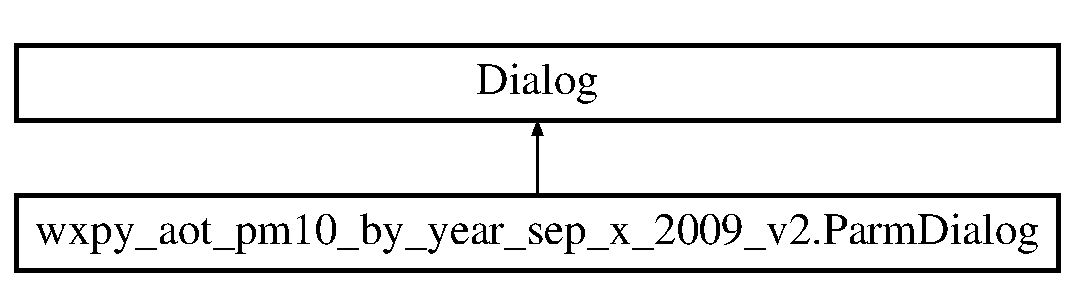
\includegraphics[height=2.000000cm]{classwxpy__aot__pm10__by__year__sep__x__2009__v2_1_1_parm_dialog}
\end{center}
\end{figure}
\subsection*{Fonctions membres publiques}
\begin{DoxyCompactItemize}
\item 
def \hyperlink{classwxpy__aot__pm10__by__year__sep__x__2009__v2_1_1_parm_dialog_a9c5514da89e4946fa0841ec6690efe8c}{\-\_\-\-\_\-init\-\_\-\-\_\-}
\item 
def \hyperlink{classwxpy__aot__pm10__by__year__sep__x__2009__v2_1_1_parm_dialog_ae016f1348d6cde5a842f3a7023ab1f4b}{Format\-Date}
\item 
def \hyperlink{classwxpy__aot__pm10__by__year__sep__x__2009__v2_1_1_parm_dialog_aac3dd041f841200317d2e42bb9cba7da}{On\-Cancel}
\item 
def \hyperlink{classwxpy__aot__pm10__by__year__sep__x__2009__v2_1_1_parm_dialog_a4eab08f0ce234ae207e2dc92c05cac8a}{On\-Ok}
\end{DoxyCompactItemize}
\subsection*{Attributs publics}
\begin{DoxyCompactItemize}
\item 
\hyperlink{classwxpy__aot__pm10__by__year__sep__x__2009__v2_1_1_parm_dialog_aee9bc2ac3794e5830a148e83cc87abc0}{Config}
\item 
\hyperlink{classwxpy__aot__pm10__by__year__sep__x__2009__v2_1_1_parm_dialog_aa3ed41206bac917476d7ce1fdd76170b}{Init\-Config}
\item 
\hyperlink{classwxpy__aot__pm10__by__year__sep__x__2009__v2_1_1_parm_dialog_af139ccb8287e43729c2057321f17968f}{b\-Change\-Config}
\item 
\hyperlink{classwxpy__aot__pm10__by__year__sep__x__2009__v2_1_1_parm_dialog_a9fa9e46076e1f62717979307e5782a18}{dpcdeb}
\item 
\hyperlink{classwxpy__aot__pm10__by__year__sep__x__2009__v2_1_1_parm_dialog_ab7cdb60dbd62e1f7296d9c993a7684ec}{dpcfin}
\item 
\hyperlink{classwxpy__aot__pm10__by__year__sep__x__2009__v2_1_1_parm_dialog_a9fef301acbdda4e13b5e195f816f7024}{spinheuredeb}
\item 
\hyperlink{classwxpy__aot__pm10__by__year__sep__x__2009__v2_1_1_parm_dialog_a437721aaac31caec2fea2c28450c3ebb}{spinheurefin}
\end{DoxyCompactItemize}


\subsection{Description détaillée}
\begin{DoxyVerb}Parameters Dialog \end{DoxyVerb}
 

\subsection{Documentation des constructeurs et destructeur}
\hypertarget{classwxpy__aot__pm10__by__year__sep__x__2009__v2_1_1_parm_dialog_a9c5514da89e4946fa0841ec6690efe8c}{\index{wxpy\-\_\-aot\-\_\-pm10\-\_\-by\-\_\-year\-\_\-sep\-\_\-x\-\_\-2009\-\_\-v2\-::\-Parm\-Dialog@{wxpy\-\_\-aot\-\_\-pm10\-\_\-by\-\_\-year\-\_\-sep\-\_\-x\-\_\-2009\-\_\-v2\-::\-Parm\-Dialog}!\-\_\-\-\_\-init\-\_\-\-\_\-@{\-\_\-\-\_\-init\-\_\-\-\_\-}}
\index{\-\_\-\-\_\-init\-\_\-\-\_\-@{\-\_\-\-\_\-init\-\_\-\-\_\-}!wxpy_aot_pm10_by_year_sep_x_2009_v2::ParmDialog@{wxpy\-\_\-aot\-\_\-pm10\-\_\-by\-\_\-year\-\_\-sep\-\_\-x\-\_\-2009\-\_\-v2\-::\-Parm\-Dialog}}
\subsubsection[{\-\_\-\-\_\-init\-\_\-\-\_\-}]{\setlength{\rightskip}{0pt plus 5cm}def wxpy\-\_\-aot\-\_\-pm10\-\_\-by\-\_\-year\-\_\-sep\-\_\-x\-\_\-2009\-\_\-v2.\-Parm\-Dialog.\-\_\-\-\_\-init\-\_\-\-\_\- (
\begin{DoxyParamCaption}
\item[{}]{self, }
\item[{}]{selframe}
\end{DoxyParamCaption}
)}}\label{classwxpy__aot__pm10__by__year__sep__x__2009__v2_1_1_parm_dialog_a9c5514da89e4946fa0841ec6690efe8c}


\subsection{Documentation des fonctions membres}
\hypertarget{classwxpy__aot__pm10__by__year__sep__x__2009__v2_1_1_parm_dialog_ae016f1348d6cde5a842f3a7023ab1f4b}{\index{wxpy\-\_\-aot\-\_\-pm10\-\_\-by\-\_\-year\-\_\-sep\-\_\-x\-\_\-2009\-\_\-v2\-::\-Parm\-Dialog@{wxpy\-\_\-aot\-\_\-pm10\-\_\-by\-\_\-year\-\_\-sep\-\_\-x\-\_\-2009\-\_\-v2\-::\-Parm\-Dialog}!Format\-Date@{Format\-Date}}
\index{Format\-Date@{Format\-Date}!wxpy_aot_pm10_by_year_sep_x_2009_v2::ParmDialog@{wxpy\-\_\-aot\-\_\-pm10\-\_\-by\-\_\-year\-\_\-sep\-\_\-x\-\_\-2009\-\_\-v2\-::\-Parm\-Dialog}}
\subsubsection[{Format\-Date}]{\setlength{\rightskip}{0pt plus 5cm}def wxpy\-\_\-aot\-\_\-pm10\-\_\-by\-\_\-year\-\_\-sep\-\_\-x\-\_\-2009\-\_\-v2.\-Parm\-Dialog.\-Format\-Date (
\begin{DoxyParamCaption}
\item[{}]{self, }
\item[{}]{date}
\end{DoxyParamCaption}
)}}\label{classwxpy__aot__pm10__by__year__sep__x__2009__v2_1_1_parm_dialog_ae016f1348d6cde5a842f3a7023ab1f4b}
\begin{DoxyVerb}Format date correctly \end{DoxyVerb}
 \hypertarget{classwxpy__aot__pm10__by__year__sep__x__2009__v2_1_1_parm_dialog_aac3dd041f841200317d2e42bb9cba7da}{\index{wxpy\-\_\-aot\-\_\-pm10\-\_\-by\-\_\-year\-\_\-sep\-\_\-x\-\_\-2009\-\_\-v2\-::\-Parm\-Dialog@{wxpy\-\_\-aot\-\_\-pm10\-\_\-by\-\_\-year\-\_\-sep\-\_\-x\-\_\-2009\-\_\-v2\-::\-Parm\-Dialog}!On\-Cancel@{On\-Cancel}}
\index{On\-Cancel@{On\-Cancel}!wxpy_aot_pm10_by_year_sep_x_2009_v2::ParmDialog@{wxpy\-\_\-aot\-\_\-pm10\-\_\-by\-\_\-year\-\_\-sep\-\_\-x\-\_\-2009\-\_\-v2\-::\-Parm\-Dialog}}
\subsubsection[{On\-Cancel}]{\setlength{\rightskip}{0pt plus 5cm}def wxpy\-\_\-aot\-\_\-pm10\-\_\-by\-\_\-year\-\_\-sep\-\_\-x\-\_\-2009\-\_\-v2.\-Parm\-Dialog.\-On\-Cancel (
\begin{DoxyParamCaption}
\item[{}]{self, }
\item[{}]{evt}
\end{DoxyParamCaption}
)}}\label{classwxpy__aot__pm10__by__year__sep__x__2009__v2_1_1_parm_dialog_aac3dd041f841200317d2e42bb9cba7da}
\hypertarget{classwxpy__aot__pm10__by__year__sep__x__2009__v2_1_1_parm_dialog_a4eab08f0ce234ae207e2dc92c05cac8a}{\index{wxpy\-\_\-aot\-\_\-pm10\-\_\-by\-\_\-year\-\_\-sep\-\_\-x\-\_\-2009\-\_\-v2\-::\-Parm\-Dialog@{wxpy\-\_\-aot\-\_\-pm10\-\_\-by\-\_\-year\-\_\-sep\-\_\-x\-\_\-2009\-\_\-v2\-::\-Parm\-Dialog}!On\-Ok@{On\-Ok}}
\index{On\-Ok@{On\-Ok}!wxpy_aot_pm10_by_year_sep_x_2009_v2::ParmDialog@{wxpy\-\_\-aot\-\_\-pm10\-\_\-by\-\_\-year\-\_\-sep\-\_\-x\-\_\-2009\-\_\-v2\-::\-Parm\-Dialog}}
\subsubsection[{On\-Ok}]{\setlength{\rightskip}{0pt plus 5cm}def wxpy\-\_\-aot\-\_\-pm10\-\_\-by\-\_\-year\-\_\-sep\-\_\-x\-\_\-2009\-\_\-v2.\-Parm\-Dialog.\-On\-Ok (
\begin{DoxyParamCaption}
\item[{}]{self, }
\item[{}]{evt}
\end{DoxyParamCaption}
)}}\label{classwxpy__aot__pm10__by__year__sep__x__2009__v2_1_1_parm_dialog_a4eab08f0ce234ae207e2dc92c05cac8a}
\begin{DoxyVerb}Confirm parameters \end{DoxyVerb}
 

\subsection{Documentation des données membres}
\hypertarget{classwxpy__aot__pm10__by__year__sep__x__2009__v2_1_1_parm_dialog_af139ccb8287e43729c2057321f17968f}{\index{wxpy\-\_\-aot\-\_\-pm10\-\_\-by\-\_\-year\-\_\-sep\-\_\-x\-\_\-2009\-\_\-v2\-::\-Parm\-Dialog@{wxpy\-\_\-aot\-\_\-pm10\-\_\-by\-\_\-year\-\_\-sep\-\_\-x\-\_\-2009\-\_\-v2\-::\-Parm\-Dialog}!b\-Change\-Config@{b\-Change\-Config}}
\index{b\-Change\-Config@{b\-Change\-Config}!wxpy_aot_pm10_by_year_sep_x_2009_v2::ParmDialog@{wxpy\-\_\-aot\-\_\-pm10\-\_\-by\-\_\-year\-\_\-sep\-\_\-x\-\_\-2009\-\_\-v2\-::\-Parm\-Dialog}}
\subsubsection[{b\-Change\-Config}]{\setlength{\rightskip}{0pt plus 5cm}wxpy\-\_\-aot\-\_\-pm10\-\_\-by\-\_\-year\-\_\-sep\-\_\-x\-\_\-2009\-\_\-v2.\-Parm\-Dialog.\-b\-Change\-Config}}\label{classwxpy__aot__pm10__by__year__sep__x__2009__v2_1_1_parm_dialog_af139ccb8287e43729c2057321f17968f}
\hypertarget{classwxpy__aot__pm10__by__year__sep__x__2009__v2_1_1_parm_dialog_aee9bc2ac3794e5830a148e83cc87abc0}{\index{wxpy\-\_\-aot\-\_\-pm10\-\_\-by\-\_\-year\-\_\-sep\-\_\-x\-\_\-2009\-\_\-v2\-::\-Parm\-Dialog@{wxpy\-\_\-aot\-\_\-pm10\-\_\-by\-\_\-year\-\_\-sep\-\_\-x\-\_\-2009\-\_\-v2\-::\-Parm\-Dialog}!Config@{Config}}
\index{Config@{Config}!wxpy_aot_pm10_by_year_sep_x_2009_v2::ParmDialog@{wxpy\-\_\-aot\-\_\-pm10\-\_\-by\-\_\-year\-\_\-sep\-\_\-x\-\_\-2009\-\_\-v2\-::\-Parm\-Dialog}}
\subsubsection[{Config}]{\setlength{\rightskip}{0pt plus 5cm}wxpy\-\_\-aot\-\_\-pm10\-\_\-by\-\_\-year\-\_\-sep\-\_\-x\-\_\-2009\-\_\-v2.\-Parm\-Dialog.\-Config}}\label{classwxpy__aot__pm10__by__year__sep__x__2009__v2_1_1_parm_dialog_aee9bc2ac3794e5830a148e83cc87abc0}
\hypertarget{classwxpy__aot__pm10__by__year__sep__x__2009__v2_1_1_parm_dialog_a9fa9e46076e1f62717979307e5782a18}{\index{wxpy\-\_\-aot\-\_\-pm10\-\_\-by\-\_\-year\-\_\-sep\-\_\-x\-\_\-2009\-\_\-v2\-::\-Parm\-Dialog@{wxpy\-\_\-aot\-\_\-pm10\-\_\-by\-\_\-year\-\_\-sep\-\_\-x\-\_\-2009\-\_\-v2\-::\-Parm\-Dialog}!dpcdeb@{dpcdeb}}
\index{dpcdeb@{dpcdeb}!wxpy_aot_pm10_by_year_sep_x_2009_v2::ParmDialog@{wxpy\-\_\-aot\-\_\-pm10\-\_\-by\-\_\-year\-\_\-sep\-\_\-x\-\_\-2009\-\_\-v2\-::\-Parm\-Dialog}}
\subsubsection[{dpcdeb}]{\setlength{\rightskip}{0pt plus 5cm}wxpy\-\_\-aot\-\_\-pm10\-\_\-by\-\_\-year\-\_\-sep\-\_\-x\-\_\-2009\-\_\-v2.\-Parm\-Dialog.\-dpcdeb}}\label{classwxpy__aot__pm10__by__year__sep__x__2009__v2_1_1_parm_dialog_a9fa9e46076e1f62717979307e5782a18}
\hypertarget{classwxpy__aot__pm10__by__year__sep__x__2009__v2_1_1_parm_dialog_ab7cdb60dbd62e1f7296d9c993a7684ec}{\index{wxpy\-\_\-aot\-\_\-pm10\-\_\-by\-\_\-year\-\_\-sep\-\_\-x\-\_\-2009\-\_\-v2\-::\-Parm\-Dialog@{wxpy\-\_\-aot\-\_\-pm10\-\_\-by\-\_\-year\-\_\-sep\-\_\-x\-\_\-2009\-\_\-v2\-::\-Parm\-Dialog}!dpcfin@{dpcfin}}
\index{dpcfin@{dpcfin}!wxpy_aot_pm10_by_year_sep_x_2009_v2::ParmDialog@{wxpy\-\_\-aot\-\_\-pm10\-\_\-by\-\_\-year\-\_\-sep\-\_\-x\-\_\-2009\-\_\-v2\-::\-Parm\-Dialog}}
\subsubsection[{dpcfin}]{\setlength{\rightskip}{0pt plus 5cm}wxpy\-\_\-aot\-\_\-pm10\-\_\-by\-\_\-year\-\_\-sep\-\_\-x\-\_\-2009\-\_\-v2.\-Parm\-Dialog.\-dpcfin}}\label{classwxpy__aot__pm10__by__year__sep__x__2009__v2_1_1_parm_dialog_ab7cdb60dbd62e1f7296d9c993a7684ec}
\hypertarget{classwxpy__aot__pm10__by__year__sep__x__2009__v2_1_1_parm_dialog_aa3ed41206bac917476d7ce1fdd76170b}{\index{wxpy\-\_\-aot\-\_\-pm10\-\_\-by\-\_\-year\-\_\-sep\-\_\-x\-\_\-2009\-\_\-v2\-::\-Parm\-Dialog@{wxpy\-\_\-aot\-\_\-pm10\-\_\-by\-\_\-year\-\_\-sep\-\_\-x\-\_\-2009\-\_\-v2\-::\-Parm\-Dialog}!Init\-Config@{Init\-Config}}
\index{Init\-Config@{Init\-Config}!wxpy_aot_pm10_by_year_sep_x_2009_v2::ParmDialog@{wxpy\-\_\-aot\-\_\-pm10\-\_\-by\-\_\-year\-\_\-sep\-\_\-x\-\_\-2009\-\_\-v2\-::\-Parm\-Dialog}}
\subsubsection[{Init\-Config}]{\setlength{\rightskip}{0pt plus 5cm}wxpy\-\_\-aot\-\_\-pm10\-\_\-by\-\_\-year\-\_\-sep\-\_\-x\-\_\-2009\-\_\-v2.\-Parm\-Dialog.\-Init\-Config}}\label{classwxpy__aot__pm10__by__year__sep__x__2009__v2_1_1_parm_dialog_aa3ed41206bac917476d7ce1fdd76170b}
\hypertarget{classwxpy__aot__pm10__by__year__sep__x__2009__v2_1_1_parm_dialog_a9fef301acbdda4e13b5e195f816f7024}{\index{wxpy\-\_\-aot\-\_\-pm10\-\_\-by\-\_\-year\-\_\-sep\-\_\-x\-\_\-2009\-\_\-v2\-::\-Parm\-Dialog@{wxpy\-\_\-aot\-\_\-pm10\-\_\-by\-\_\-year\-\_\-sep\-\_\-x\-\_\-2009\-\_\-v2\-::\-Parm\-Dialog}!spinheuredeb@{spinheuredeb}}
\index{spinheuredeb@{spinheuredeb}!wxpy_aot_pm10_by_year_sep_x_2009_v2::ParmDialog@{wxpy\-\_\-aot\-\_\-pm10\-\_\-by\-\_\-year\-\_\-sep\-\_\-x\-\_\-2009\-\_\-v2\-::\-Parm\-Dialog}}
\subsubsection[{spinheuredeb}]{\setlength{\rightskip}{0pt plus 5cm}wxpy\-\_\-aot\-\_\-pm10\-\_\-by\-\_\-year\-\_\-sep\-\_\-x\-\_\-2009\-\_\-v2.\-Parm\-Dialog.\-spinheuredeb}}\label{classwxpy__aot__pm10__by__year__sep__x__2009__v2_1_1_parm_dialog_a9fef301acbdda4e13b5e195f816f7024}
\hypertarget{classwxpy__aot__pm10__by__year__sep__x__2009__v2_1_1_parm_dialog_a437721aaac31caec2fea2c28450c3ebb}{\index{wxpy\-\_\-aot\-\_\-pm10\-\_\-by\-\_\-year\-\_\-sep\-\_\-x\-\_\-2009\-\_\-v2\-::\-Parm\-Dialog@{wxpy\-\_\-aot\-\_\-pm10\-\_\-by\-\_\-year\-\_\-sep\-\_\-x\-\_\-2009\-\_\-v2\-::\-Parm\-Dialog}!spinheurefin@{spinheurefin}}
\index{spinheurefin@{spinheurefin}!wxpy_aot_pm10_by_year_sep_x_2009_v2::ParmDialog@{wxpy\-\_\-aot\-\_\-pm10\-\_\-by\-\_\-year\-\_\-sep\-\_\-x\-\_\-2009\-\_\-v2\-::\-Parm\-Dialog}}
\subsubsection[{spinheurefin}]{\setlength{\rightskip}{0pt plus 5cm}wxpy\-\_\-aot\-\_\-pm10\-\_\-by\-\_\-year\-\_\-sep\-\_\-x\-\_\-2009\-\_\-v2.\-Parm\-Dialog.\-spinheurefin}}\label{classwxpy__aot__pm10__by__year__sep__x__2009__v2_1_1_parm_dialog_a437721aaac31caec2fea2c28450c3ebb}


La documentation de cette classe a été générée à partir du fichier suivant \-:\begin{DoxyCompactItemize}
\item 
\hyperlink{wxpy__aot__pm10__by__year__sep__x__2009__v2_8py}{wxpy\-\_\-aot\-\_\-pm10\-\_\-by\-\_\-year\-\_\-sep\-\_\-x\-\_\-2009\-\_\-v2.\-py}\end{DoxyCompactItemize}

\hypertarget{classwxpy__aot__pm10__by__month_1_1_parm_dialog}{\section{Référence de la classe wxpy\-\_\-aot\-\_\-pm10\-\_\-by\-\_\-month.\-Parm\-Dialog}
\label{classwxpy__aot__pm10__by__month_1_1_parm_dialog}\index{wxpy\-\_\-aot\-\_\-pm10\-\_\-by\-\_\-month.\-Parm\-Dialog@{wxpy\-\_\-aot\-\_\-pm10\-\_\-by\-\_\-month.\-Parm\-Dialog}}
}
Graphe d'héritage de wxpy\-\_\-aot\-\_\-pm10\-\_\-by\-\_\-month.\-Parm\-Dialog\-:\begin{figure}[H]
\begin{center}
\leavevmode
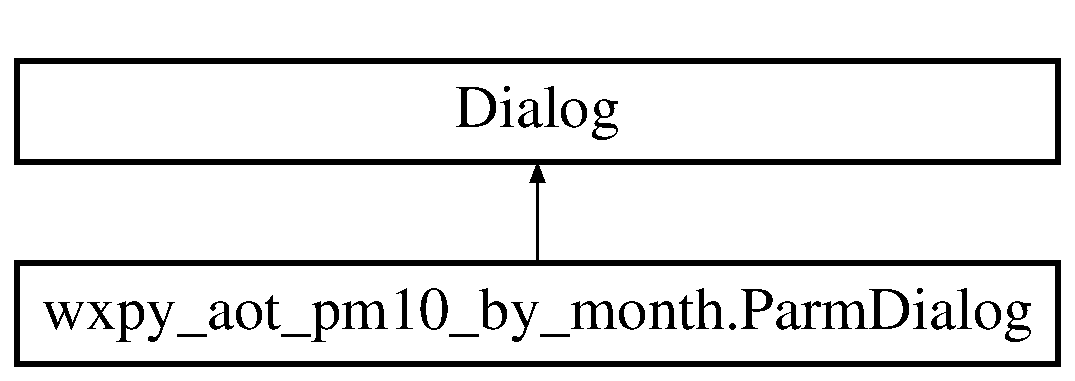
\includegraphics[height=2.000000cm]{classwxpy__aot__pm10__by__month_1_1_parm_dialog}
\end{center}
\end{figure}
\subsection*{Fonctions membres publiques}
\begin{DoxyCompactItemize}
\item 
def \hyperlink{classwxpy__aot__pm10__by__month_1_1_parm_dialog_a8695ab9eea88c4cd85400b58af5c4a99}{\-\_\-\-\_\-init\-\_\-\-\_\-}
\item 
def \hyperlink{classwxpy__aot__pm10__by__month_1_1_parm_dialog_a0d2482b2a3170196d3c4aab90e25596e}{Format\-Date}
\item 
def \hyperlink{classwxpy__aot__pm10__by__month_1_1_parm_dialog_a51a1ad23e3c387bb92052d66d4a99071}{On\-Cancel}
\item 
def \hyperlink{classwxpy__aot__pm10__by__month_1_1_parm_dialog_a329d7ab5ad3a0881df2614a9e485801e}{On\-Ok}
\end{DoxyCompactItemize}
\subsection*{Attributs publics}
\begin{DoxyCompactItemize}
\item 
\hyperlink{classwxpy__aot__pm10__by__month_1_1_parm_dialog_a8a8a41f0d5ab617775c581231b790fa5}{Config}
\item 
\hyperlink{classwxpy__aot__pm10__by__month_1_1_parm_dialog_ac26f18b5304e9f076593bdfb3db03920}{Init\-Config}
\item 
\hyperlink{classwxpy__aot__pm10__by__month_1_1_parm_dialog_abe053ac189afa9eacc3b1d6de8a79ae8}{b\-Change\-Config}
\item 
\hyperlink{classwxpy__aot__pm10__by__month_1_1_parm_dialog_ada722a70ebf9e134003d0bc54977348d}{dpcdeb}
\item 
\hyperlink{classwxpy__aot__pm10__by__month_1_1_parm_dialog_afe230e911ec35ffff2e5c0250fb1c830}{dpcfin}
\item 
\hyperlink{classwxpy__aot__pm10__by__month_1_1_parm_dialog_ad56b6700ee49f8e7ae04bc8614f46e53}{spinheuredeb}
\item 
\hyperlink{classwxpy__aot__pm10__by__month_1_1_parm_dialog_a7a132b6b24ffbe92f8527b953b2b0fa1}{spinheurefin}
\end{DoxyCompactItemize}


\subsection{Description détaillée}
\begin{DoxyVerb}Parameters Dialog \end{DoxyVerb}
 

\subsection{Documentation des constructeurs et destructeur}
\hypertarget{classwxpy__aot__pm10__by__month_1_1_parm_dialog_a8695ab9eea88c4cd85400b58af5c4a99}{\index{wxpy\-\_\-aot\-\_\-pm10\-\_\-by\-\_\-month\-::\-Parm\-Dialog@{wxpy\-\_\-aot\-\_\-pm10\-\_\-by\-\_\-month\-::\-Parm\-Dialog}!\-\_\-\-\_\-init\-\_\-\-\_\-@{\-\_\-\-\_\-init\-\_\-\-\_\-}}
\index{\-\_\-\-\_\-init\-\_\-\-\_\-@{\-\_\-\-\_\-init\-\_\-\-\_\-}!wxpy_aot_pm10_by_month::ParmDialog@{wxpy\-\_\-aot\-\_\-pm10\-\_\-by\-\_\-month\-::\-Parm\-Dialog}}
\subsubsection[{\-\_\-\-\_\-init\-\_\-\-\_\-}]{\setlength{\rightskip}{0pt plus 5cm}def wxpy\-\_\-aot\-\_\-pm10\-\_\-by\-\_\-month.\-Parm\-Dialog.\-\_\-\-\_\-init\-\_\-\-\_\- (
\begin{DoxyParamCaption}
\item[{}]{self, }
\item[{}]{selframe}
\end{DoxyParamCaption}
)}}\label{classwxpy__aot__pm10__by__month_1_1_parm_dialog_a8695ab9eea88c4cd85400b58af5c4a99}


\subsection{Documentation des fonctions membres}
\hypertarget{classwxpy__aot__pm10__by__month_1_1_parm_dialog_a0d2482b2a3170196d3c4aab90e25596e}{\index{wxpy\-\_\-aot\-\_\-pm10\-\_\-by\-\_\-month\-::\-Parm\-Dialog@{wxpy\-\_\-aot\-\_\-pm10\-\_\-by\-\_\-month\-::\-Parm\-Dialog}!Format\-Date@{Format\-Date}}
\index{Format\-Date@{Format\-Date}!wxpy_aot_pm10_by_month::ParmDialog@{wxpy\-\_\-aot\-\_\-pm10\-\_\-by\-\_\-month\-::\-Parm\-Dialog}}
\subsubsection[{Format\-Date}]{\setlength{\rightskip}{0pt plus 5cm}def wxpy\-\_\-aot\-\_\-pm10\-\_\-by\-\_\-month.\-Parm\-Dialog.\-Format\-Date (
\begin{DoxyParamCaption}
\item[{}]{self, }
\item[{}]{date}
\end{DoxyParamCaption}
)}}\label{classwxpy__aot__pm10__by__month_1_1_parm_dialog_a0d2482b2a3170196d3c4aab90e25596e}
\begin{DoxyVerb}Format date correctly \end{DoxyVerb}
 \hypertarget{classwxpy__aot__pm10__by__month_1_1_parm_dialog_a51a1ad23e3c387bb92052d66d4a99071}{\index{wxpy\-\_\-aot\-\_\-pm10\-\_\-by\-\_\-month\-::\-Parm\-Dialog@{wxpy\-\_\-aot\-\_\-pm10\-\_\-by\-\_\-month\-::\-Parm\-Dialog}!On\-Cancel@{On\-Cancel}}
\index{On\-Cancel@{On\-Cancel}!wxpy_aot_pm10_by_month::ParmDialog@{wxpy\-\_\-aot\-\_\-pm10\-\_\-by\-\_\-month\-::\-Parm\-Dialog}}
\subsubsection[{On\-Cancel}]{\setlength{\rightskip}{0pt plus 5cm}def wxpy\-\_\-aot\-\_\-pm10\-\_\-by\-\_\-month.\-Parm\-Dialog.\-On\-Cancel (
\begin{DoxyParamCaption}
\item[{}]{self, }
\item[{}]{evt}
\end{DoxyParamCaption}
)}}\label{classwxpy__aot__pm10__by__month_1_1_parm_dialog_a51a1ad23e3c387bb92052d66d4a99071}
\hypertarget{classwxpy__aot__pm10__by__month_1_1_parm_dialog_a329d7ab5ad3a0881df2614a9e485801e}{\index{wxpy\-\_\-aot\-\_\-pm10\-\_\-by\-\_\-month\-::\-Parm\-Dialog@{wxpy\-\_\-aot\-\_\-pm10\-\_\-by\-\_\-month\-::\-Parm\-Dialog}!On\-Ok@{On\-Ok}}
\index{On\-Ok@{On\-Ok}!wxpy_aot_pm10_by_month::ParmDialog@{wxpy\-\_\-aot\-\_\-pm10\-\_\-by\-\_\-month\-::\-Parm\-Dialog}}
\subsubsection[{On\-Ok}]{\setlength{\rightskip}{0pt plus 5cm}def wxpy\-\_\-aot\-\_\-pm10\-\_\-by\-\_\-month.\-Parm\-Dialog.\-On\-Ok (
\begin{DoxyParamCaption}
\item[{}]{self, }
\item[{}]{evt}
\end{DoxyParamCaption}
)}}\label{classwxpy__aot__pm10__by__month_1_1_parm_dialog_a329d7ab5ad3a0881df2614a9e485801e}
\begin{DoxyVerb}Confirm parameters \end{DoxyVerb}
 

\subsection{Documentation des données membres}
\hypertarget{classwxpy__aot__pm10__by__month_1_1_parm_dialog_abe053ac189afa9eacc3b1d6de8a79ae8}{\index{wxpy\-\_\-aot\-\_\-pm10\-\_\-by\-\_\-month\-::\-Parm\-Dialog@{wxpy\-\_\-aot\-\_\-pm10\-\_\-by\-\_\-month\-::\-Parm\-Dialog}!b\-Change\-Config@{b\-Change\-Config}}
\index{b\-Change\-Config@{b\-Change\-Config}!wxpy_aot_pm10_by_month::ParmDialog@{wxpy\-\_\-aot\-\_\-pm10\-\_\-by\-\_\-month\-::\-Parm\-Dialog}}
\subsubsection[{b\-Change\-Config}]{\setlength{\rightskip}{0pt plus 5cm}wxpy\-\_\-aot\-\_\-pm10\-\_\-by\-\_\-month.\-Parm\-Dialog.\-b\-Change\-Config}}\label{classwxpy__aot__pm10__by__month_1_1_parm_dialog_abe053ac189afa9eacc3b1d6de8a79ae8}
\hypertarget{classwxpy__aot__pm10__by__month_1_1_parm_dialog_a8a8a41f0d5ab617775c581231b790fa5}{\index{wxpy\-\_\-aot\-\_\-pm10\-\_\-by\-\_\-month\-::\-Parm\-Dialog@{wxpy\-\_\-aot\-\_\-pm10\-\_\-by\-\_\-month\-::\-Parm\-Dialog}!Config@{Config}}
\index{Config@{Config}!wxpy_aot_pm10_by_month::ParmDialog@{wxpy\-\_\-aot\-\_\-pm10\-\_\-by\-\_\-month\-::\-Parm\-Dialog}}
\subsubsection[{Config}]{\setlength{\rightskip}{0pt plus 5cm}wxpy\-\_\-aot\-\_\-pm10\-\_\-by\-\_\-month.\-Parm\-Dialog.\-Config}}\label{classwxpy__aot__pm10__by__month_1_1_parm_dialog_a8a8a41f0d5ab617775c581231b790fa5}
\hypertarget{classwxpy__aot__pm10__by__month_1_1_parm_dialog_ada722a70ebf9e134003d0bc54977348d}{\index{wxpy\-\_\-aot\-\_\-pm10\-\_\-by\-\_\-month\-::\-Parm\-Dialog@{wxpy\-\_\-aot\-\_\-pm10\-\_\-by\-\_\-month\-::\-Parm\-Dialog}!dpcdeb@{dpcdeb}}
\index{dpcdeb@{dpcdeb}!wxpy_aot_pm10_by_month::ParmDialog@{wxpy\-\_\-aot\-\_\-pm10\-\_\-by\-\_\-month\-::\-Parm\-Dialog}}
\subsubsection[{dpcdeb}]{\setlength{\rightskip}{0pt plus 5cm}wxpy\-\_\-aot\-\_\-pm10\-\_\-by\-\_\-month.\-Parm\-Dialog.\-dpcdeb}}\label{classwxpy__aot__pm10__by__month_1_1_parm_dialog_ada722a70ebf9e134003d0bc54977348d}
\hypertarget{classwxpy__aot__pm10__by__month_1_1_parm_dialog_afe230e911ec35ffff2e5c0250fb1c830}{\index{wxpy\-\_\-aot\-\_\-pm10\-\_\-by\-\_\-month\-::\-Parm\-Dialog@{wxpy\-\_\-aot\-\_\-pm10\-\_\-by\-\_\-month\-::\-Parm\-Dialog}!dpcfin@{dpcfin}}
\index{dpcfin@{dpcfin}!wxpy_aot_pm10_by_month::ParmDialog@{wxpy\-\_\-aot\-\_\-pm10\-\_\-by\-\_\-month\-::\-Parm\-Dialog}}
\subsubsection[{dpcfin}]{\setlength{\rightskip}{0pt plus 5cm}wxpy\-\_\-aot\-\_\-pm10\-\_\-by\-\_\-month.\-Parm\-Dialog.\-dpcfin}}\label{classwxpy__aot__pm10__by__month_1_1_parm_dialog_afe230e911ec35ffff2e5c0250fb1c830}
\hypertarget{classwxpy__aot__pm10__by__month_1_1_parm_dialog_ac26f18b5304e9f076593bdfb3db03920}{\index{wxpy\-\_\-aot\-\_\-pm10\-\_\-by\-\_\-month\-::\-Parm\-Dialog@{wxpy\-\_\-aot\-\_\-pm10\-\_\-by\-\_\-month\-::\-Parm\-Dialog}!Init\-Config@{Init\-Config}}
\index{Init\-Config@{Init\-Config}!wxpy_aot_pm10_by_month::ParmDialog@{wxpy\-\_\-aot\-\_\-pm10\-\_\-by\-\_\-month\-::\-Parm\-Dialog}}
\subsubsection[{Init\-Config}]{\setlength{\rightskip}{0pt plus 5cm}wxpy\-\_\-aot\-\_\-pm10\-\_\-by\-\_\-month.\-Parm\-Dialog.\-Init\-Config}}\label{classwxpy__aot__pm10__by__month_1_1_parm_dialog_ac26f18b5304e9f076593bdfb3db03920}
\hypertarget{classwxpy__aot__pm10__by__month_1_1_parm_dialog_ad56b6700ee49f8e7ae04bc8614f46e53}{\index{wxpy\-\_\-aot\-\_\-pm10\-\_\-by\-\_\-month\-::\-Parm\-Dialog@{wxpy\-\_\-aot\-\_\-pm10\-\_\-by\-\_\-month\-::\-Parm\-Dialog}!spinheuredeb@{spinheuredeb}}
\index{spinheuredeb@{spinheuredeb}!wxpy_aot_pm10_by_month::ParmDialog@{wxpy\-\_\-aot\-\_\-pm10\-\_\-by\-\_\-month\-::\-Parm\-Dialog}}
\subsubsection[{spinheuredeb}]{\setlength{\rightskip}{0pt plus 5cm}wxpy\-\_\-aot\-\_\-pm10\-\_\-by\-\_\-month.\-Parm\-Dialog.\-spinheuredeb}}\label{classwxpy__aot__pm10__by__month_1_1_parm_dialog_ad56b6700ee49f8e7ae04bc8614f46e53}
\hypertarget{classwxpy__aot__pm10__by__month_1_1_parm_dialog_a7a132b6b24ffbe92f8527b953b2b0fa1}{\index{wxpy\-\_\-aot\-\_\-pm10\-\_\-by\-\_\-month\-::\-Parm\-Dialog@{wxpy\-\_\-aot\-\_\-pm10\-\_\-by\-\_\-month\-::\-Parm\-Dialog}!spinheurefin@{spinheurefin}}
\index{spinheurefin@{spinheurefin}!wxpy_aot_pm10_by_month::ParmDialog@{wxpy\-\_\-aot\-\_\-pm10\-\_\-by\-\_\-month\-::\-Parm\-Dialog}}
\subsubsection[{spinheurefin}]{\setlength{\rightskip}{0pt plus 5cm}wxpy\-\_\-aot\-\_\-pm10\-\_\-by\-\_\-month.\-Parm\-Dialog.\-spinheurefin}}\label{classwxpy__aot__pm10__by__month_1_1_parm_dialog_a7a132b6b24ffbe92f8527b953b2b0fa1}


La documentation de cette classe a été générée à partir du fichier suivant \-:\begin{DoxyCompactItemize}
\item 
\hyperlink{wxpy__aot__pm10__by__month_8py}{wxpy\-\_\-aot\-\_\-pm10\-\_\-by\-\_\-month.\-py}\end{DoxyCompactItemize}

\hypertarget{classwxpy__aot__pm10__by__years_1_1_parm_dialog}{\section{Référence de la classe wxpy\-\_\-aot\-\_\-pm10\-\_\-by\-\_\-years.\-Parm\-Dialog}
\label{classwxpy__aot__pm10__by__years_1_1_parm_dialog}\index{wxpy\-\_\-aot\-\_\-pm10\-\_\-by\-\_\-years.\-Parm\-Dialog@{wxpy\-\_\-aot\-\_\-pm10\-\_\-by\-\_\-years.\-Parm\-Dialog}}
}
Graphe d'héritage de wxpy\-\_\-aot\-\_\-pm10\-\_\-by\-\_\-years.\-Parm\-Dialog\-:\begin{figure}[H]
\begin{center}
\leavevmode
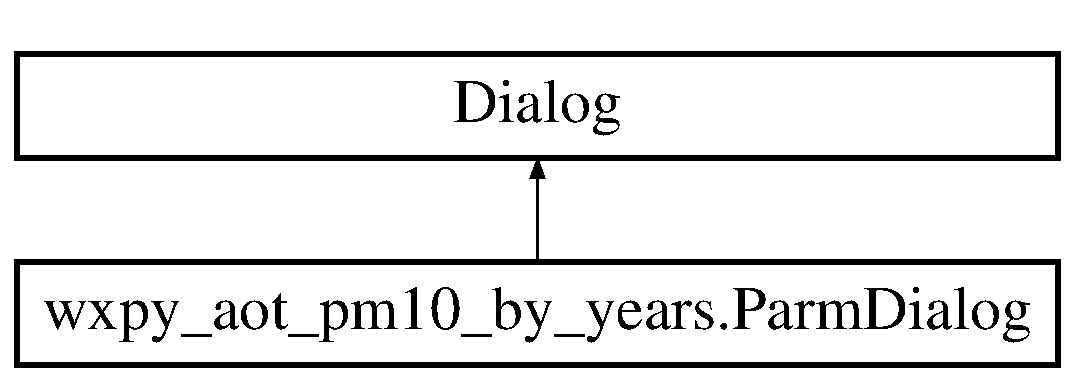
\includegraphics[height=2.000000cm]{classwxpy__aot__pm10__by__years_1_1_parm_dialog}
\end{center}
\end{figure}
\subsection*{Fonctions membres publiques}
\begin{DoxyCompactItemize}
\item 
def \hyperlink{classwxpy__aot__pm10__by__years_1_1_parm_dialog_aaf8aad9aa96ec759ff1dbf2c4ac43063}{\-\_\-\-\_\-init\-\_\-\-\_\-}
\item 
def \hyperlink{classwxpy__aot__pm10__by__years_1_1_parm_dialog_a137d3b0e70159fe1f3d5e2682f9ffb65}{Format\-Date}
\item 
def \hyperlink{classwxpy__aot__pm10__by__years_1_1_parm_dialog_a81eb27d16e4b864d27f63754f0321658}{On\-Cancel}
\item 
def \hyperlink{classwxpy__aot__pm10__by__years_1_1_parm_dialog_a1d6fcb1a8cc75fd53d045d0352c17a28}{On\-Ok}
\end{DoxyCompactItemize}
\subsection*{Attributs publics}
\begin{DoxyCompactItemize}
\item 
\hyperlink{classwxpy__aot__pm10__by__years_1_1_parm_dialog_a8f46610bc4e19567f9748510186ed54e}{Config}
\item 
\hyperlink{classwxpy__aot__pm10__by__years_1_1_parm_dialog_a38c43c3d7e72ae31a284ecd0d0a734e0}{Init\-Config}
\item 
\hyperlink{classwxpy__aot__pm10__by__years_1_1_parm_dialog_a4c2543a042150133d99fb7a8be4bc2cf}{b\-Change\-Config}
\item 
\hyperlink{classwxpy__aot__pm10__by__years_1_1_parm_dialog_a4ccab1c487bf3983e40469f2b8f113ff}{dpcdeb}
\item 
\hyperlink{classwxpy__aot__pm10__by__years_1_1_parm_dialog_a3859975e0a07319b6ee7836af13bc910}{dpcfin}
\item 
\hyperlink{classwxpy__aot__pm10__by__years_1_1_parm_dialog_ab1c0e372077c2cc87041a5a941cd9ece}{spinheuredeb}
\item 
\hyperlink{classwxpy__aot__pm10__by__years_1_1_parm_dialog_ac5ee9d047f733153e00caa48d1ed0772}{spinheurefin}
\end{DoxyCompactItemize}


\subsection{Description détaillée}
\begin{DoxyVerb}Parameters Dialog \end{DoxyVerb}
 

\subsection{Documentation des constructeurs et destructeur}
\hypertarget{classwxpy__aot__pm10__by__years_1_1_parm_dialog_aaf8aad9aa96ec759ff1dbf2c4ac43063}{\index{wxpy\-\_\-aot\-\_\-pm10\-\_\-by\-\_\-years\-::\-Parm\-Dialog@{wxpy\-\_\-aot\-\_\-pm10\-\_\-by\-\_\-years\-::\-Parm\-Dialog}!\-\_\-\-\_\-init\-\_\-\-\_\-@{\-\_\-\-\_\-init\-\_\-\-\_\-}}
\index{\-\_\-\-\_\-init\-\_\-\-\_\-@{\-\_\-\-\_\-init\-\_\-\-\_\-}!wxpy_aot_pm10_by_years::ParmDialog@{wxpy\-\_\-aot\-\_\-pm10\-\_\-by\-\_\-years\-::\-Parm\-Dialog}}
\subsubsection[{\-\_\-\-\_\-init\-\_\-\-\_\-}]{\setlength{\rightskip}{0pt plus 5cm}def wxpy\-\_\-aot\-\_\-pm10\-\_\-by\-\_\-years.\-Parm\-Dialog.\-\_\-\-\_\-init\-\_\-\-\_\- (
\begin{DoxyParamCaption}
\item[{}]{self, }
\item[{}]{selframe}
\end{DoxyParamCaption}
)}}\label{classwxpy__aot__pm10__by__years_1_1_parm_dialog_aaf8aad9aa96ec759ff1dbf2c4ac43063}


\subsection{Documentation des fonctions membres}
\hypertarget{classwxpy__aot__pm10__by__years_1_1_parm_dialog_a137d3b0e70159fe1f3d5e2682f9ffb65}{\index{wxpy\-\_\-aot\-\_\-pm10\-\_\-by\-\_\-years\-::\-Parm\-Dialog@{wxpy\-\_\-aot\-\_\-pm10\-\_\-by\-\_\-years\-::\-Parm\-Dialog}!Format\-Date@{Format\-Date}}
\index{Format\-Date@{Format\-Date}!wxpy_aot_pm10_by_years::ParmDialog@{wxpy\-\_\-aot\-\_\-pm10\-\_\-by\-\_\-years\-::\-Parm\-Dialog}}
\subsubsection[{Format\-Date}]{\setlength{\rightskip}{0pt plus 5cm}def wxpy\-\_\-aot\-\_\-pm10\-\_\-by\-\_\-years.\-Parm\-Dialog.\-Format\-Date (
\begin{DoxyParamCaption}
\item[{}]{self, }
\item[{}]{date}
\end{DoxyParamCaption}
)}}\label{classwxpy__aot__pm10__by__years_1_1_parm_dialog_a137d3b0e70159fe1f3d5e2682f9ffb65}
\begin{DoxyVerb}Format date correctly \end{DoxyVerb}
 \hypertarget{classwxpy__aot__pm10__by__years_1_1_parm_dialog_a81eb27d16e4b864d27f63754f0321658}{\index{wxpy\-\_\-aot\-\_\-pm10\-\_\-by\-\_\-years\-::\-Parm\-Dialog@{wxpy\-\_\-aot\-\_\-pm10\-\_\-by\-\_\-years\-::\-Parm\-Dialog}!On\-Cancel@{On\-Cancel}}
\index{On\-Cancel@{On\-Cancel}!wxpy_aot_pm10_by_years::ParmDialog@{wxpy\-\_\-aot\-\_\-pm10\-\_\-by\-\_\-years\-::\-Parm\-Dialog}}
\subsubsection[{On\-Cancel}]{\setlength{\rightskip}{0pt plus 5cm}def wxpy\-\_\-aot\-\_\-pm10\-\_\-by\-\_\-years.\-Parm\-Dialog.\-On\-Cancel (
\begin{DoxyParamCaption}
\item[{}]{self, }
\item[{}]{evt}
\end{DoxyParamCaption}
)}}\label{classwxpy__aot__pm10__by__years_1_1_parm_dialog_a81eb27d16e4b864d27f63754f0321658}
\hypertarget{classwxpy__aot__pm10__by__years_1_1_parm_dialog_a1d6fcb1a8cc75fd53d045d0352c17a28}{\index{wxpy\-\_\-aot\-\_\-pm10\-\_\-by\-\_\-years\-::\-Parm\-Dialog@{wxpy\-\_\-aot\-\_\-pm10\-\_\-by\-\_\-years\-::\-Parm\-Dialog}!On\-Ok@{On\-Ok}}
\index{On\-Ok@{On\-Ok}!wxpy_aot_pm10_by_years::ParmDialog@{wxpy\-\_\-aot\-\_\-pm10\-\_\-by\-\_\-years\-::\-Parm\-Dialog}}
\subsubsection[{On\-Ok}]{\setlength{\rightskip}{0pt plus 5cm}def wxpy\-\_\-aot\-\_\-pm10\-\_\-by\-\_\-years.\-Parm\-Dialog.\-On\-Ok (
\begin{DoxyParamCaption}
\item[{}]{self, }
\item[{}]{evt}
\end{DoxyParamCaption}
)}}\label{classwxpy__aot__pm10__by__years_1_1_parm_dialog_a1d6fcb1a8cc75fd53d045d0352c17a28}
\begin{DoxyVerb}Confirm parameters \end{DoxyVerb}
 

\subsection{Documentation des données membres}
\hypertarget{classwxpy__aot__pm10__by__years_1_1_parm_dialog_a4c2543a042150133d99fb7a8be4bc2cf}{\index{wxpy\-\_\-aot\-\_\-pm10\-\_\-by\-\_\-years\-::\-Parm\-Dialog@{wxpy\-\_\-aot\-\_\-pm10\-\_\-by\-\_\-years\-::\-Parm\-Dialog}!b\-Change\-Config@{b\-Change\-Config}}
\index{b\-Change\-Config@{b\-Change\-Config}!wxpy_aot_pm10_by_years::ParmDialog@{wxpy\-\_\-aot\-\_\-pm10\-\_\-by\-\_\-years\-::\-Parm\-Dialog}}
\subsubsection[{b\-Change\-Config}]{\setlength{\rightskip}{0pt plus 5cm}wxpy\-\_\-aot\-\_\-pm10\-\_\-by\-\_\-years.\-Parm\-Dialog.\-b\-Change\-Config}}\label{classwxpy__aot__pm10__by__years_1_1_parm_dialog_a4c2543a042150133d99fb7a8be4bc2cf}
\hypertarget{classwxpy__aot__pm10__by__years_1_1_parm_dialog_a8f46610bc4e19567f9748510186ed54e}{\index{wxpy\-\_\-aot\-\_\-pm10\-\_\-by\-\_\-years\-::\-Parm\-Dialog@{wxpy\-\_\-aot\-\_\-pm10\-\_\-by\-\_\-years\-::\-Parm\-Dialog}!Config@{Config}}
\index{Config@{Config}!wxpy_aot_pm10_by_years::ParmDialog@{wxpy\-\_\-aot\-\_\-pm10\-\_\-by\-\_\-years\-::\-Parm\-Dialog}}
\subsubsection[{Config}]{\setlength{\rightskip}{0pt plus 5cm}wxpy\-\_\-aot\-\_\-pm10\-\_\-by\-\_\-years.\-Parm\-Dialog.\-Config}}\label{classwxpy__aot__pm10__by__years_1_1_parm_dialog_a8f46610bc4e19567f9748510186ed54e}
\hypertarget{classwxpy__aot__pm10__by__years_1_1_parm_dialog_a4ccab1c487bf3983e40469f2b8f113ff}{\index{wxpy\-\_\-aot\-\_\-pm10\-\_\-by\-\_\-years\-::\-Parm\-Dialog@{wxpy\-\_\-aot\-\_\-pm10\-\_\-by\-\_\-years\-::\-Parm\-Dialog}!dpcdeb@{dpcdeb}}
\index{dpcdeb@{dpcdeb}!wxpy_aot_pm10_by_years::ParmDialog@{wxpy\-\_\-aot\-\_\-pm10\-\_\-by\-\_\-years\-::\-Parm\-Dialog}}
\subsubsection[{dpcdeb}]{\setlength{\rightskip}{0pt plus 5cm}wxpy\-\_\-aot\-\_\-pm10\-\_\-by\-\_\-years.\-Parm\-Dialog.\-dpcdeb}}\label{classwxpy__aot__pm10__by__years_1_1_parm_dialog_a4ccab1c487bf3983e40469f2b8f113ff}
\hypertarget{classwxpy__aot__pm10__by__years_1_1_parm_dialog_a3859975e0a07319b6ee7836af13bc910}{\index{wxpy\-\_\-aot\-\_\-pm10\-\_\-by\-\_\-years\-::\-Parm\-Dialog@{wxpy\-\_\-aot\-\_\-pm10\-\_\-by\-\_\-years\-::\-Parm\-Dialog}!dpcfin@{dpcfin}}
\index{dpcfin@{dpcfin}!wxpy_aot_pm10_by_years::ParmDialog@{wxpy\-\_\-aot\-\_\-pm10\-\_\-by\-\_\-years\-::\-Parm\-Dialog}}
\subsubsection[{dpcfin}]{\setlength{\rightskip}{0pt plus 5cm}wxpy\-\_\-aot\-\_\-pm10\-\_\-by\-\_\-years.\-Parm\-Dialog.\-dpcfin}}\label{classwxpy__aot__pm10__by__years_1_1_parm_dialog_a3859975e0a07319b6ee7836af13bc910}
\hypertarget{classwxpy__aot__pm10__by__years_1_1_parm_dialog_a38c43c3d7e72ae31a284ecd0d0a734e0}{\index{wxpy\-\_\-aot\-\_\-pm10\-\_\-by\-\_\-years\-::\-Parm\-Dialog@{wxpy\-\_\-aot\-\_\-pm10\-\_\-by\-\_\-years\-::\-Parm\-Dialog}!Init\-Config@{Init\-Config}}
\index{Init\-Config@{Init\-Config}!wxpy_aot_pm10_by_years::ParmDialog@{wxpy\-\_\-aot\-\_\-pm10\-\_\-by\-\_\-years\-::\-Parm\-Dialog}}
\subsubsection[{Init\-Config}]{\setlength{\rightskip}{0pt plus 5cm}wxpy\-\_\-aot\-\_\-pm10\-\_\-by\-\_\-years.\-Parm\-Dialog.\-Init\-Config}}\label{classwxpy__aot__pm10__by__years_1_1_parm_dialog_a38c43c3d7e72ae31a284ecd0d0a734e0}
\hypertarget{classwxpy__aot__pm10__by__years_1_1_parm_dialog_ab1c0e372077c2cc87041a5a941cd9ece}{\index{wxpy\-\_\-aot\-\_\-pm10\-\_\-by\-\_\-years\-::\-Parm\-Dialog@{wxpy\-\_\-aot\-\_\-pm10\-\_\-by\-\_\-years\-::\-Parm\-Dialog}!spinheuredeb@{spinheuredeb}}
\index{spinheuredeb@{spinheuredeb}!wxpy_aot_pm10_by_years::ParmDialog@{wxpy\-\_\-aot\-\_\-pm10\-\_\-by\-\_\-years\-::\-Parm\-Dialog}}
\subsubsection[{spinheuredeb}]{\setlength{\rightskip}{0pt plus 5cm}wxpy\-\_\-aot\-\_\-pm10\-\_\-by\-\_\-years.\-Parm\-Dialog.\-spinheuredeb}}\label{classwxpy__aot__pm10__by__years_1_1_parm_dialog_ab1c0e372077c2cc87041a5a941cd9ece}
\hypertarget{classwxpy__aot__pm10__by__years_1_1_parm_dialog_ac5ee9d047f733153e00caa48d1ed0772}{\index{wxpy\-\_\-aot\-\_\-pm10\-\_\-by\-\_\-years\-::\-Parm\-Dialog@{wxpy\-\_\-aot\-\_\-pm10\-\_\-by\-\_\-years\-::\-Parm\-Dialog}!spinheurefin@{spinheurefin}}
\index{spinheurefin@{spinheurefin}!wxpy_aot_pm10_by_years::ParmDialog@{wxpy\-\_\-aot\-\_\-pm10\-\_\-by\-\_\-years\-::\-Parm\-Dialog}}
\subsubsection[{spinheurefin}]{\setlength{\rightskip}{0pt plus 5cm}wxpy\-\_\-aot\-\_\-pm10\-\_\-by\-\_\-years.\-Parm\-Dialog.\-spinheurefin}}\label{classwxpy__aot__pm10__by__years_1_1_parm_dialog_ac5ee9d047f733153e00caa48d1ed0772}


La documentation de cette classe a été générée à partir du fichier suivant \-:\begin{DoxyCompactItemize}
\item 
\hyperlink{wxpy__aot__pm10__by__years_8py}{wxpy\-\_\-aot\-\_\-pm10\-\_\-by\-\_\-years.\-py}\end{DoxyCompactItemize}

\hypertarget{classwxpy__aot__pm10__by__year__sep__x__2009__v2_1_1selmat}{\section{Référence de la classe wxpy\-\_\-aot\-\_\-pm10\-\_\-by\-\_\-year\-\_\-sep\-\_\-x\-\_\-2009\-\_\-v2.\-selmat}
\label{classwxpy__aot__pm10__by__year__sep__x__2009__v2_1_1selmat}\index{wxpy\-\_\-aot\-\_\-pm10\-\_\-by\-\_\-year\-\_\-sep\-\_\-x\-\_\-2009\-\_\-v2.\-selmat@{wxpy\-\_\-aot\-\_\-pm10\-\_\-by\-\_\-year\-\_\-sep\-\_\-x\-\_\-2009\-\_\-v2.\-selmat}}
}
\subsection*{Fonctions membres publiques}
\begin{DoxyCompactItemize}
\item 
def \hyperlink{classwxpy__aot__pm10__by__year__sep__x__2009__v2_1_1selmat_a66bcb5ab38d0a1c471208b65f22b9cb5}{\-\_\-\-\_\-init\-\_\-\-\_\-}
\end{DoxyCompactItemize}
\subsection*{Attributs publics}
\begin{DoxyCompactItemize}
\item 
\hyperlink{classwxpy__aot__pm10__by__year__sep__x__2009__v2_1_1selmat_a15e02ca0f998d05c6eb07057f7547265}{sourcemat}
\item 
\hyperlink{classwxpy__aot__pm10__by__year__sep__x__2009__v2_1_1selmat_a7fec5adb0cd9a35b68ba77e044603c29}{lstlimits}
\end{DoxyCompactItemize}


\subsection{Description détaillée}
\begin{DoxyVerb}Renvoyer un extrait de matrice (array) \end{DoxyVerb}
 

\subsection{Documentation des constructeurs et destructeur}
\hypertarget{classwxpy__aot__pm10__by__year__sep__x__2009__v2_1_1selmat_a66bcb5ab38d0a1c471208b65f22b9cb5}{\index{wxpy\-\_\-aot\-\_\-pm10\-\_\-by\-\_\-year\-\_\-sep\-\_\-x\-\_\-2009\-\_\-v2\-::selmat@{wxpy\-\_\-aot\-\_\-pm10\-\_\-by\-\_\-year\-\_\-sep\-\_\-x\-\_\-2009\-\_\-v2\-::selmat}!\-\_\-\-\_\-init\-\_\-\-\_\-@{\-\_\-\-\_\-init\-\_\-\-\_\-}}
\index{\-\_\-\-\_\-init\-\_\-\-\_\-@{\-\_\-\-\_\-init\-\_\-\-\_\-}!wxpy_aot_pm10_by_year_sep_x_2009_v2::selmat@{wxpy\-\_\-aot\-\_\-pm10\-\_\-by\-\_\-year\-\_\-sep\-\_\-x\-\_\-2009\-\_\-v2\-::selmat}}
\subsubsection[{\-\_\-\-\_\-init\-\_\-\-\_\-}]{\setlength{\rightskip}{0pt plus 5cm}def wxpy\-\_\-aot\-\_\-pm10\-\_\-by\-\_\-year\-\_\-sep\-\_\-x\-\_\-2009\-\_\-v2.\-selmat.\-\_\-\-\_\-init\-\_\-\-\_\- (
\begin{DoxyParamCaption}
\item[{}]{self, }
\item[{}]{sourcemat, }
\item[{}]{lstlimits}
\end{DoxyParamCaption}
)}}\label{classwxpy__aot__pm10__by__year__sep__x__2009__v2_1_1selmat_a66bcb5ab38d0a1c471208b65f22b9cb5}


\subsection{Documentation des données membres}
\hypertarget{classwxpy__aot__pm10__by__year__sep__x__2009__v2_1_1selmat_a7fec5adb0cd9a35b68ba77e044603c29}{\index{wxpy\-\_\-aot\-\_\-pm10\-\_\-by\-\_\-year\-\_\-sep\-\_\-x\-\_\-2009\-\_\-v2\-::selmat@{wxpy\-\_\-aot\-\_\-pm10\-\_\-by\-\_\-year\-\_\-sep\-\_\-x\-\_\-2009\-\_\-v2\-::selmat}!lstlimits@{lstlimits}}
\index{lstlimits@{lstlimits}!wxpy_aot_pm10_by_year_sep_x_2009_v2::selmat@{wxpy\-\_\-aot\-\_\-pm10\-\_\-by\-\_\-year\-\_\-sep\-\_\-x\-\_\-2009\-\_\-v2\-::selmat}}
\subsubsection[{lstlimits}]{\setlength{\rightskip}{0pt plus 5cm}wxpy\-\_\-aot\-\_\-pm10\-\_\-by\-\_\-year\-\_\-sep\-\_\-x\-\_\-2009\-\_\-v2.\-selmat.\-lstlimits}}\label{classwxpy__aot__pm10__by__year__sep__x__2009__v2_1_1selmat_a7fec5adb0cd9a35b68ba77e044603c29}
\hypertarget{classwxpy__aot__pm10__by__year__sep__x__2009__v2_1_1selmat_a15e02ca0f998d05c6eb07057f7547265}{\index{wxpy\-\_\-aot\-\_\-pm10\-\_\-by\-\_\-year\-\_\-sep\-\_\-x\-\_\-2009\-\_\-v2\-::selmat@{wxpy\-\_\-aot\-\_\-pm10\-\_\-by\-\_\-year\-\_\-sep\-\_\-x\-\_\-2009\-\_\-v2\-::selmat}!sourcemat@{sourcemat}}
\index{sourcemat@{sourcemat}!wxpy_aot_pm10_by_year_sep_x_2009_v2::selmat@{wxpy\-\_\-aot\-\_\-pm10\-\_\-by\-\_\-year\-\_\-sep\-\_\-x\-\_\-2009\-\_\-v2\-::selmat}}
\subsubsection[{sourcemat}]{\setlength{\rightskip}{0pt plus 5cm}wxpy\-\_\-aot\-\_\-pm10\-\_\-by\-\_\-year\-\_\-sep\-\_\-x\-\_\-2009\-\_\-v2.\-selmat.\-sourcemat}}\label{classwxpy__aot__pm10__by__year__sep__x__2009__v2_1_1selmat_a15e02ca0f998d05c6eb07057f7547265}


La documentation de cette classe a été générée à partir du fichier suivant \-:\begin{DoxyCompactItemize}
\item 
\hyperlink{wxpy__aot__pm10__by__year__sep__x__2009__v2_8py}{wxpy\-\_\-aot\-\_\-pm10\-\_\-by\-\_\-year\-\_\-sep\-\_\-x\-\_\-2009\-\_\-v2.\-py}\end{DoxyCompactItemize}

\hypertarget{classwxpy__aot__pm10__by__month_1_1selmat}{\section{Référence de la classe wxpy\-\_\-aot\-\_\-pm10\-\_\-by\-\_\-month.\-selmat}
\label{classwxpy__aot__pm10__by__month_1_1selmat}\index{wxpy\-\_\-aot\-\_\-pm10\-\_\-by\-\_\-month.\-selmat@{wxpy\-\_\-aot\-\_\-pm10\-\_\-by\-\_\-month.\-selmat}}
}
\subsection*{Fonctions membres publiques}
\begin{DoxyCompactItemize}
\item 
def \hyperlink{classwxpy__aot__pm10__by__month_1_1selmat_a1f44457b40f609e39e7f330cd4c0e669}{\-\_\-\-\_\-init\-\_\-\-\_\-}
\end{DoxyCompactItemize}
\subsection*{Attributs publics}
\begin{DoxyCompactItemize}
\item 
\hyperlink{classwxpy__aot__pm10__by__month_1_1selmat_a91b6cf14ce6fdab2c952f05773900a47}{sourcemat}
\item 
\hyperlink{classwxpy__aot__pm10__by__month_1_1selmat_a14381ca92cfac6add3dfaddab060b68e}{lstlimits}
\end{DoxyCompactItemize}


\subsection{Description détaillée}
\begin{DoxyVerb}Renvoyer un extrait de matrice (array) \end{DoxyVerb}
 

\subsection{Documentation des constructeurs et destructeur}
\hypertarget{classwxpy__aot__pm10__by__month_1_1selmat_a1f44457b40f609e39e7f330cd4c0e669}{\index{wxpy\-\_\-aot\-\_\-pm10\-\_\-by\-\_\-month\-::selmat@{wxpy\-\_\-aot\-\_\-pm10\-\_\-by\-\_\-month\-::selmat}!\-\_\-\-\_\-init\-\_\-\-\_\-@{\-\_\-\-\_\-init\-\_\-\-\_\-}}
\index{\-\_\-\-\_\-init\-\_\-\-\_\-@{\-\_\-\-\_\-init\-\_\-\-\_\-}!wxpy_aot_pm10_by_month::selmat@{wxpy\-\_\-aot\-\_\-pm10\-\_\-by\-\_\-month\-::selmat}}
\subsubsection[{\-\_\-\-\_\-init\-\_\-\-\_\-}]{\setlength{\rightskip}{0pt plus 5cm}def wxpy\-\_\-aot\-\_\-pm10\-\_\-by\-\_\-month.\-selmat.\-\_\-\-\_\-init\-\_\-\-\_\- (
\begin{DoxyParamCaption}
\item[{}]{self, }
\item[{}]{sourcemat, }
\item[{}]{lstlimits}
\end{DoxyParamCaption}
)}}\label{classwxpy__aot__pm10__by__month_1_1selmat_a1f44457b40f609e39e7f330cd4c0e669}


\subsection{Documentation des données membres}
\hypertarget{classwxpy__aot__pm10__by__month_1_1selmat_a14381ca92cfac6add3dfaddab060b68e}{\index{wxpy\-\_\-aot\-\_\-pm10\-\_\-by\-\_\-month\-::selmat@{wxpy\-\_\-aot\-\_\-pm10\-\_\-by\-\_\-month\-::selmat}!lstlimits@{lstlimits}}
\index{lstlimits@{lstlimits}!wxpy_aot_pm10_by_month::selmat@{wxpy\-\_\-aot\-\_\-pm10\-\_\-by\-\_\-month\-::selmat}}
\subsubsection[{lstlimits}]{\setlength{\rightskip}{0pt plus 5cm}wxpy\-\_\-aot\-\_\-pm10\-\_\-by\-\_\-month.\-selmat.\-lstlimits}}\label{classwxpy__aot__pm10__by__month_1_1selmat_a14381ca92cfac6add3dfaddab060b68e}
\hypertarget{classwxpy__aot__pm10__by__month_1_1selmat_a91b6cf14ce6fdab2c952f05773900a47}{\index{wxpy\-\_\-aot\-\_\-pm10\-\_\-by\-\_\-month\-::selmat@{wxpy\-\_\-aot\-\_\-pm10\-\_\-by\-\_\-month\-::selmat}!sourcemat@{sourcemat}}
\index{sourcemat@{sourcemat}!wxpy_aot_pm10_by_month::selmat@{wxpy\-\_\-aot\-\_\-pm10\-\_\-by\-\_\-month\-::selmat}}
\subsubsection[{sourcemat}]{\setlength{\rightskip}{0pt plus 5cm}wxpy\-\_\-aot\-\_\-pm10\-\_\-by\-\_\-month.\-selmat.\-sourcemat}}\label{classwxpy__aot__pm10__by__month_1_1selmat_a91b6cf14ce6fdab2c952f05773900a47}


La documentation de cette classe a été générée à partir du fichier suivant \-:\begin{DoxyCompactItemize}
\item 
\hyperlink{wxpy__aot__pm10__by__month_8py}{wxpy\-\_\-aot\-\_\-pm10\-\_\-by\-\_\-month.\-py}\end{DoxyCompactItemize}

\hypertarget{classwxpy__aot__pm10__by__years_1_1selmat}{\section{Référence de la classe wxpy\-\_\-aot\-\_\-pm10\-\_\-by\-\_\-years.\-selmat}
\label{classwxpy__aot__pm10__by__years_1_1selmat}\index{wxpy\-\_\-aot\-\_\-pm10\-\_\-by\-\_\-years.\-selmat@{wxpy\-\_\-aot\-\_\-pm10\-\_\-by\-\_\-years.\-selmat}}
}
\subsection*{Fonctions membres publiques}
\begin{DoxyCompactItemize}
\item 
def \hyperlink{classwxpy__aot__pm10__by__years_1_1selmat_a71298a7382194b0646dedcc77bcd22ed}{\-\_\-\-\_\-init\-\_\-\-\_\-}
\end{DoxyCompactItemize}
\subsection*{Attributs publics}
\begin{DoxyCompactItemize}
\item 
\hyperlink{classwxpy__aot__pm10__by__years_1_1selmat_a63ae225a45883227129fecbf1b726c75}{sourcemat}
\item 
\hyperlink{classwxpy__aot__pm10__by__years_1_1selmat_a0538fd4db9267578887d2aba3c3629c3}{lstlimits}
\end{DoxyCompactItemize}


\subsection{Description détaillée}
\begin{DoxyVerb}Renvoyer un extrait de matrice (array) \end{DoxyVerb}
 

\subsection{Documentation des constructeurs et destructeur}
\hypertarget{classwxpy__aot__pm10__by__years_1_1selmat_a71298a7382194b0646dedcc77bcd22ed}{\index{wxpy\-\_\-aot\-\_\-pm10\-\_\-by\-\_\-years\-::selmat@{wxpy\-\_\-aot\-\_\-pm10\-\_\-by\-\_\-years\-::selmat}!\-\_\-\-\_\-init\-\_\-\-\_\-@{\-\_\-\-\_\-init\-\_\-\-\_\-}}
\index{\-\_\-\-\_\-init\-\_\-\-\_\-@{\-\_\-\-\_\-init\-\_\-\-\_\-}!wxpy_aot_pm10_by_years::selmat@{wxpy\-\_\-aot\-\_\-pm10\-\_\-by\-\_\-years\-::selmat}}
\subsubsection[{\-\_\-\-\_\-init\-\_\-\-\_\-}]{\setlength{\rightskip}{0pt plus 5cm}def wxpy\-\_\-aot\-\_\-pm10\-\_\-by\-\_\-years.\-selmat.\-\_\-\-\_\-init\-\_\-\-\_\- (
\begin{DoxyParamCaption}
\item[{}]{self, }
\item[{}]{sourcemat, }
\item[{}]{lstlimits}
\end{DoxyParamCaption}
)}}\label{classwxpy__aot__pm10__by__years_1_1selmat_a71298a7382194b0646dedcc77bcd22ed}


\subsection{Documentation des données membres}
\hypertarget{classwxpy__aot__pm10__by__years_1_1selmat_a0538fd4db9267578887d2aba3c3629c3}{\index{wxpy\-\_\-aot\-\_\-pm10\-\_\-by\-\_\-years\-::selmat@{wxpy\-\_\-aot\-\_\-pm10\-\_\-by\-\_\-years\-::selmat}!lstlimits@{lstlimits}}
\index{lstlimits@{lstlimits}!wxpy_aot_pm10_by_years::selmat@{wxpy\-\_\-aot\-\_\-pm10\-\_\-by\-\_\-years\-::selmat}}
\subsubsection[{lstlimits}]{\setlength{\rightskip}{0pt plus 5cm}wxpy\-\_\-aot\-\_\-pm10\-\_\-by\-\_\-years.\-selmat.\-lstlimits}}\label{classwxpy__aot__pm10__by__years_1_1selmat_a0538fd4db9267578887d2aba3c3629c3}
\hypertarget{classwxpy__aot__pm10__by__years_1_1selmat_a63ae225a45883227129fecbf1b726c75}{\index{wxpy\-\_\-aot\-\_\-pm10\-\_\-by\-\_\-years\-::selmat@{wxpy\-\_\-aot\-\_\-pm10\-\_\-by\-\_\-years\-::selmat}!sourcemat@{sourcemat}}
\index{sourcemat@{sourcemat}!wxpy_aot_pm10_by_years::selmat@{wxpy\-\_\-aot\-\_\-pm10\-\_\-by\-\_\-years\-::selmat}}
\subsubsection[{sourcemat}]{\setlength{\rightskip}{0pt plus 5cm}wxpy\-\_\-aot\-\_\-pm10\-\_\-by\-\_\-years.\-selmat.\-sourcemat}}\label{classwxpy__aot__pm10__by__years_1_1selmat_a63ae225a45883227129fecbf1b726c75}


La documentation de cette classe a été générée à partir du fichier suivant \-:\begin{DoxyCompactItemize}
\item 
\hyperlink{wxpy__aot__pm10__by__years_8py}{wxpy\-\_\-aot\-\_\-pm10\-\_\-by\-\_\-years.\-py}\end{DoxyCompactItemize}

\chapter{Documentation des fichiers}
\hypertarget{datefromday_8py}{\section{Référence du fichier datefromday.\-py}
\label{datefromday_8py}\index{datefromday.\-py@{datefromday.\-py}}
}
\subsection*{Classes}
\begin{DoxyCompactItemize}
\item 
class \hyperlink{classdatefromday_1_1datefromday}{datefromday.\-datefromday}
\end{DoxyCompactItemize}
\subsection*{Espaces de nommage}
\begin{DoxyCompactItemize}
\item 
namespace \hyperlink{namespacedatefromday}{datefromday}
\end{DoxyCompactItemize}
\subsection*{Variables}
\begin{DoxyCompactItemize}
\item 
int \hyperlink{namespacedatefromday_aede275c34345c420325ebc297aba81f9}{datefromday.\-day} = 182
\item 
int \hyperlink{namespacedatefromday_a7919c99d6443529b833c52f4cfea8419}{datefromday.\-year} = 2005
\item 
tuple \hyperlink{namespacedatefromday_a5f8d14af9c7da65685fd0496da5174eb}{datefromday.\-dd} = datefromday(year,day)
\end{DoxyCompactItemize}

\hypertarget{dayfromdate_8py}{\section{Référence du fichier dayfromdate.\-py}
\label{dayfromdate_8py}\index{dayfromdate.\-py@{dayfromdate.\-py}}
}
\subsection*{Classes}
\begin{DoxyCompactItemize}
\item 
class \hyperlink{classdayfromdate_1_1dayfromdate}{dayfromdate.\-dayfromdate}
\end{DoxyCompactItemize}
\subsection*{Espaces de nommage}
\begin{DoxyCompactItemize}
\item 
namespace \hyperlink{namespacedayfromdate}{dayfromdate}
\end{DoxyCompactItemize}
\subsection*{Variables}
\begin{DoxyCompactItemize}
\item 
tuple \hyperlink{namespacedayfromdate_aff2b24216941c68bc2f62c556efb05ce}{dayfromdate.\-date} = dayfromdate(2005,7,1)
\end{DoxyCompactItemize}

\hypertarget{wxpy__aot__pm10__by__month_8py}{\section{Référence du fichier wxpy\-\_\-aot\-\_\-pm10\-\_\-by\-\_\-month.\-py}
\label{wxpy__aot__pm10__by__month_8py}\index{wxpy\-\_\-aot\-\_\-pm10\-\_\-by\-\_\-month.\-py@{wxpy\-\_\-aot\-\_\-pm10\-\_\-by\-\_\-month.\-py}}
}
\subsection*{Classes}
\begin{DoxyCompactItemize}
\item 
class \hyperlink{classwxpy__aot__pm10__by__month_1_1selmat}{wxpy\-\_\-aot\-\_\-pm10\-\_\-by\-\_\-month.\-selmat}
\item 
class \hyperlink{classwxpy__aot__pm10__by__month_1_1_my_navigation_toolbar}{wxpy\-\_\-aot\-\_\-pm10\-\_\-by\-\_\-month.\-My\-Navigation\-Toolbar}
\item 
class \hyperlink{classwxpy__aot__pm10__by__month_1_1_parm_dialog}{wxpy\-\_\-aot\-\_\-pm10\-\_\-by\-\_\-month.\-Parm\-Dialog}
\item 
class \hyperlink{classwxpy__aot__pm10__by__month_1_1_canvas_frame}{wxpy\-\_\-aot\-\_\-pm10\-\_\-by\-\_\-month.\-Canvas\-Frame}
\item 
class \hyperlink{classwxpy__aot__pm10__by__month_1_1_app}{wxpy\-\_\-aot\-\_\-pm10\-\_\-by\-\_\-month.\-App}
\end{DoxyCompactItemize}
\subsection*{Espaces de nommage}
\begin{DoxyCompactItemize}
\item 
namespace \hyperlink{namespacewxpy__aot__pm10__by__month}{wxpy\-\_\-aot\-\_\-pm10\-\_\-by\-\_\-month}
\end{DoxyCompactItemize}
\subsection*{Variables}
\begin{DoxyCompactItemize}
\item 
tuple \hyperlink{namespacewxpy__aot__pm10__by__month_a65e5a097e1930719563f1a64776f4b79}{wxpy\-\_\-aot\-\_\-pm10\-\_\-by\-\_\-month.\-app} = App(redirect=False)
\end{DoxyCompactItemize}

\hypertarget{wxpy__aot__pm10__by__year__sep__x__2009__v2_8py}{\section{Référence du fichier wxpy\-\_\-aot\-\_\-pm10\-\_\-by\-\_\-year\-\_\-sep\-\_\-x\-\_\-2009\-\_\-v2.\-py}
\label{wxpy__aot__pm10__by__year__sep__x__2009__v2_8py}\index{wxpy\-\_\-aot\-\_\-pm10\-\_\-by\-\_\-year\-\_\-sep\-\_\-x\-\_\-2009\-\_\-v2.\-py@{wxpy\-\_\-aot\-\_\-pm10\-\_\-by\-\_\-year\-\_\-sep\-\_\-x\-\_\-2009\-\_\-v2.\-py}}
}
\subsection*{Classes}
\begin{DoxyCompactItemize}
\item 
class \hyperlink{classwxpy__aot__pm10__by__year__sep__x__2009__v2_1_1selmat}{wxpy\-\_\-aot\-\_\-pm10\-\_\-by\-\_\-year\-\_\-sep\-\_\-x\-\_\-2009\-\_\-v2.\-selmat}
\item 
class \hyperlink{classwxpy__aot__pm10__by__year__sep__x__2009__v2_1_1_my_navigation_toolbar}{wxpy\-\_\-aot\-\_\-pm10\-\_\-by\-\_\-year\-\_\-sep\-\_\-x\-\_\-2009\-\_\-v2.\-My\-Navigation\-Toolbar}
\item 
class \hyperlink{classwxpy__aot__pm10__by__year__sep__x__2009__v2_1_1_parm_dialog}{wxpy\-\_\-aot\-\_\-pm10\-\_\-by\-\_\-year\-\_\-sep\-\_\-x\-\_\-2009\-\_\-v2.\-Parm\-Dialog}
\item 
class \hyperlink{classwxpy__aot__pm10__by__year__sep__x__2009__v2_1_1_canvas_frame}{wxpy\-\_\-aot\-\_\-pm10\-\_\-by\-\_\-year\-\_\-sep\-\_\-x\-\_\-2009\-\_\-v2.\-Canvas\-Frame}
\item 
class \hyperlink{classwxpy__aot__pm10__by__year__sep__x__2009__v2_1_1_app}{wxpy\-\_\-aot\-\_\-pm10\-\_\-by\-\_\-year\-\_\-sep\-\_\-x\-\_\-2009\-\_\-v2.\-App}
\end{DoxyCompactItemize}
\subsection*{Espaces de nommage}
\begin{DoxyCompactItemize}
\item 
namespace \hyperlink{namespacewxpy__aot__pm10__by__year__sep__x__2009__v2}{wxpy\-\_\-aot\-\_\-pm10\-\_\-by\-\_\-year\-\_\-sep\-\_\-x\-\_\-2009\-\_\-v2}
\end{DoxyCompactItemize}
\subsection*{Variables}
\begin{DoxyCompactItemize}
\item 
tuple \hyperlink{namespacewxpy__aot__pm10__by__year__sep__x__2009__v2_ab35478ac0294be440bd6850a9d621f87}{wxpy\-\_\-aot\-\_\-pm10\-\_\-by\-\_\-year\-\_\-sep\-\_\-x\-\_\-2009\-\_\-v2.\-app} = App(redirect=False)
\end{DoxyCompactItemize}

\hypertarget{wxpy__aot__pm10__by__years_8py}{\section{Référence du fichier wxpy\-\_\-aot\-\_\-pm10\-\_\-by\-\_\-years.\-py}
\label{wxpy__aot__pm10__by__years_8py}\index{wxpy\-\_\-aot\-\_\-pm10\-\_\-by\-\_\-years.\-py@{wxpy\-\_\-aot\-\_\-pm10\-\_\-by\-\_\-years.\-py}}
}
\subsection*{Classes}
\begin{DoxyCompactItemize}
\item 
class \hyperlink{classwxpy__aot__pm10__by__years_1_1selmat}{wxpy\-\_\-aot\-\_\-pm10\-\_\-by\-\_\-years.\-selmat}
\item 
class \hyperlink{classwxpy__aot__pm10__by__years_1_1_my_navigation_toolbar}{wxpy\-\_\-aot\-\_\-pm10\-\_\-by\-\_\-years.\-My\-Navigation\-Toolbar}
\item 
class \hyperlink{classwxpy__aot__pm10__by__years_1_1_parm_dialog}{wxpy\-\_\-aot\-\_\-pm10\-\_\-by\-\_\-years.\-Parm\-Dialog}
\item 
class \hyperlink{classwxpy__aot__pm10__by__years_1_1_canvas_frame}{wxpy\-\_\-aot\-\_\-pm10\-\_\-by\-\_\-years.\-Canvas\-Frame}
\item 
class \hyperlink{classwxpy__aot__pm10__by__years_1_1_app}{wxpy\-\_\-aot\-\_\-pm10\-\_\-by\-\_\-years.\-App}
\end{DoxyCompactItemize}
\subsection*{Espaces de nommage}
\begin{DoxyCompactItemize}
\item 
namespace \hyperlink{namespacewxpy__aot__pm10__by__years}{wxpy\-\_\-aot\-\_\-pm10\-\_\-by\-\_\-years}
\end{DoxyCompactItemize}
\subsection*{Variables}
\begin{DoxyCompactItemize}
\item 
tuple \hyperlink{namespacewxpy__aot__pm10__by__years_ae73f95ecf03aafc7416828159ebbc5db}{wxpy\-\_\-aot\-\_\-pm10\-\_\-by\-\_\-years.\-app} = App(redirect=False)
\end{DoxyCompactItemize}

\addcontentsline{toc}{part}{Index}
\printindex
\end{document}
